% Options for packages loaded elsewhere
\PassOptionsToPackage{unicode}{hyperref}
\PassOptionsToPackage{hyphens}{url}
%
\documentclass[
  12 pt,
]{book}
\usepackage{amsmath,amssymb}
\usepackage{iftex}
\ifPDFTeX
  \usepackage[T1]{fontenc}
  \usepackage[utf8]{inputenc}
  \usepackage{textcomp} % provide euro and other symbols
\else % if luatex or xetex
  \usepackage{unicode-math} % this also loads fontspec
  \defaultfontfeatures{Scale=MatchLowercase}
  \defaultfontfeatures[\rmfamily]{Ligatures=TeX,Scale=1}
\fi
\usepackage{lmodern}
\ifPDFTeX\else
  % xetex/luatex font selection
\fi
% Use upquote if available, for straight quotes in verbatim environments
\IfFileExists{upquote.sty}{\usepackage{upquote}}{}
\IfFileExists{microtype.sty}{% use microtype if available
  \usepackage[]{microtype}
  \UseMicrotypeSet[protrusion]{basicmath} % disable protrusion for tt fonts
}{}
\makeatletter
\@ifundefined{KOMAClassName}{% if non-KOMA class
  \IfFileExists{parskip.sty}{%
    \usepackage{parskip}
  }{% else
    \setlength{\parindent}{0pt}
    \setlength{\parskip}{6pt plus 2pt minus 1pt}}
}{% if KOMA class
  \KOMAoptions{parskip=half}}
\makeatother
\usepackage{xcolor}
\usepackage{longtable,booktabs,array}
\usepackage{calc} % for calculating minipage widths
% Correct order of tables after \paragraph or \subparagraph
\usepackage{etoolbox}
\makeatletter
\patchcmd\longtable{\par}{\if@noskipsec\mbox{}\fi\par}{}{}
\makeatother
% Allow footnotes in longtable head/foot
\IfFileExists{footnotehyper.sty}{\usepackage{footnotehyper}}{\usepackage{footnote}}
\makesavenoteenv{longtable}
\usepackage{graphicx}
\makeatletter
\def\maxwidth{\ifdim\Gin@nat@width>\linewidth\linewidth\else\Gin@nat@width\fi}
\def\maxheight{\ifdim\Gin@nat@height>\textheight\textheight\else\Gin@nat@height\fi}
\makeatother
% Scale images if necessary, so that they will not overflow the page
% margins by default, and it is still possible to overwrite the defaults
% using explicit options in \includegraphics[width, height, ...]{}
\setkeys{Gin}{width=\maxwidth,height=\maxheight,keepaspectratio}
% Set default figure placement to htbp
\makeatletter
\def\fps@figure{htbp}
\makeatother
\setlength{\emergencystretch}{3em} % prevent overfull lines
\providecommand{\tightlist}{%
  \setlength{\itemsep}{0pt}\setlength{\parskip}{0pt}}
\setcounter{secnumdepth}{5}
\newlength{\cslhangindent}
\setlength{\cslhangindent}{1.5em}
\newlength{\csllabelwidth}
\setlength{\csllabelwidth}{3em}
\newlength{\cslentryspacingunit} % times entry-spacing
\setlength{\cslentryspacingunit}{\parskip}
\newenvironment{CSLReferences}[2] % #1 hanging-ident, #2 entry spacing
 {% don't indent paragraphs
  \setlength{\parindent}{0pt}
  % turn on hanging indent if param 1 is 1
  \ifodd #1
  \let\oldpar\par
  \def\par{\hangindent=\cslhangindent\oldpar}
  \fi
  % set entry spacing
  \setlength{\parskip}{#2\cslentryspacingunit}
 }%
 {}
\usepackage{calc}
\newcommand{\CSLBlock}[1]{#1\hfill\break}
\newcommand{\CSLLeftMargin}[1]{\parbox[t]{\csllabelwidth}{#1}}
\newcommand{\CSLRightInline}[1]{\parbox[t]{\linewidth - \csllabelwidth}{#1}\break}
\newcommand{\CSLIndent}[1]{\hspace{\cslhangindent}#1}
%%%%%%%%%%%%%%%%%%%%%%%%%%%%%%%%%%%%%%%%%%%%%%%%%%%%%%%%%%%%
% Font
%%%%%%%%%%%%%%%%%%%%%%%%%%%%%%%%%%%%%%%%%%%%%%%%%%%%%%%%%%%%

% Set font encoding to T1 (8-bit encoding, 256 glyphs) 
% (improved text handling, especially with non-English
% languages and text containing special characters)
\usepackage[T1]{fontenc}

% Set font to URW Nimbus Roman
% (Times New Roman alternative)
\usepackage{mathptmx}

% Include the Helvetica font and scale the font to 92% of
% its original size (used to better fit the Times like font 
% provided by mathptmx)
\usepackage[scaled=0.92]{helvet}

%%%%%%%%%%%%%%%%%%%%%%%%%%%%%%%%%%%%%%%%%%%%%%%%%%%%%%%%%%%%
% Title page
%%%%%%%%%%%%%%%%%%%%%%%%%%%%%%%%%%%%%%%%%%%%%%%%%%%%%%%%%%%%

% Turn off \maketitle so that we can customise
% the title pages
\AtBeginDocument{\let\maketitle\relax}

% Define macros to customise the title pages
\makeatletter
% Define macro for title in Croatian
\def\HRtitle#1{\gdef\@HRtitle{#1}}
\def\@HRtitle{\@latex@warning@no@line{No \noexpand\HRtitle given}}
% Define macro for faculty name in English
\def\ENfaculty#1{\gdef\@ENfaculty{#1}}
\def\@ENfaculty{\@latex@warning@no@line{No \noexpand\ENfaculty given}}
% Define macro for faculty name in Croatian
\def\HRfaculty#1{\gdef\@HRfaculty{#1}}
\def\@HRfaculty{\@latex@warning@no@line{No \noexpand\HRfaculty given}}
% Define macro for department name in English
\def\ENdepartment#1{\gdef\@ENdepartment{#1}}
\def\@ENdepartment{\@latex@warning@no@line{No \noexpand\ENdepartment given}}
% Define macro for department name in Croatian
\def\HRdepartment#1{\gdef\@HRdepartment{#1}}
\def\@HRdepartment{\@latex@warning@no@line{No \noexpand\HRdepartment given}}
% Define macro for supervisor name and title in English
\def\ENsupervisor#1{\gdef\@ENsupervisor{#1}}
\def\@ENsupervisor{\@latex@warning@no@line{No \noexpand\ENsupervisor given}}
% Define macro for supervisor name and title in Croatian
\def\HRsupervisor#1{\gdef\@HRsupervisor{#1}}
\def\@HRsupervisor{\@latex@warning@no@line{No \noexpand\HRsupervisor given}}
% Define macro for place
\def\place#1{\gdef\@place{#1}}
\def\@place{\@latex@warning@no@line{No \noexpand\place given}}
\makeatother

%%%%%%%%%%%%%%%%%%%%%%%%%%%%%%%%%%%%%%%%%%%%%%%%%%%%%%%%%%%%
% Table of contents (TOC), list of figures (LOF),
% and list of tables (LOT)
%%%%%%%%%%%%%%%%%%%%%%%%%%%%%%%%%%%%%%%%%%%%%%%%%%%%%%%%%%%%

% Include package providing additional functionality for TOC
% customisation
\usepackage{titletoc}

% Define the number of levels in the TOC
\setcounter{tocdepth}{4}

% Ensure that the dotted ruler in the TOC goes all the way
% to the number
\contentsmargin[2.8em]{0em}
\renewcommand\contentspage{\thecontentspage}

% Customise the appearance of the chapter level
\titlecontents{chapter}
    [1.0em] % text indentation
    {\addvspace{0em}} % vertical space before entry
    {\contentslabel{1.0em}} % set the format and indentation
                            % of the numbered entries
    {\hspace*{-1.0em}} % set the format and indentation
                       % of the numberless entries
    {\titlerule*[0.4pc]{.}\contentspage} % format the horizontal rule

% Customise the appearance of the section level
\titlecontents{section}
    [2.8em] % text indentation (i.e., 1.0em (chapter) + 1.8em)
    {\addvspace{0em}} % vertical space before entry
    {\contentslabel{1.8em}} % set the format and indentation
                            % of the numbered entries
    {\hspace*{-1.8em}} % set the format and indentation
                       % of the numberless entries
    {\titlerule*[0.4pc]{.}\contentspage} % format the horizontal rule

% Customise the appearance of the subsection level
\titlecontents{subsection}
    [5.5em] % text indentation (i.e., 2.8em (section) + 2.7em)
    {\addvspace{0em}} % vertical space before entry
    {\contentslabel{2.7em}} % set the format and indentation
                            % of the numbered entries
    {\hspace*{-2.7em}} % set the format and indentation
                       % of the numberless entries
    {\titlerule*[0.4pc]{.}\contentspage} % format the horizontal rule

% Customise the appearance of the subsubsection level    
\titlecontents{subsubsection}
    [9.1em] % text indentation (i.e., 5.5em (subsection) + 3.6em)
    {\addvspace{0em}} % vertical space before entry
    {\contentslabel{3.6em}} % set the format and indentation
                            % of the numbered entries
    {\hspace*{-3.6em}} % set the format and indentation
                       % of the numberless entries
    {\titlerule*[0.4pc]{.}\contentspage} % format the horizontal rule

%%%%%%%%%%%%%%%%%%%%%%%%%%%%%%%%%%%%%%%%%%%%%%%%%%%%%%%%%%%%
% Typsetting
%%%%%%%%%%%%%%%%%%%%%%%%%%%%%%%%%%%%%%%%%%%%%%%%%%%%%%%%%%%%

% Include the geometry package to set various layout parameters
% of the document, such as paper size, margins, and more
% (here, we set the paper size, the size of the margins, and
% define wheter the document has to be single or double sided)
\usepackage[
% Uncomment the following line to visualise the layout of the
% document by drawing frames around the various areas, such as
% the text area, margins, headers, and footers
%showframe,
paper=a4paper, twoside=false,
top=2.5cm, bottom=2.5cm, right=2.5cm, left=2.5cm]{geometry}

% Include package to create landscape-oriented pages
\usepackage{pdflscape}

% Include the package allowing the load of external
% multi-page PDF documents in LaTeX documents
\usepackage{pdfpages}

% Include package providing fine-tuned typographic enhancements
\usepackage{microtype}

% Include package for text alignment
% (provides refinements which improve the standard LaTeX
% alignemnt commands and environments)
\usepackage{ragged2e}

% Supress hyphenation
\usepackage[none]{hyphenat}

% Include package for setting spacing between lines
\usepackage{setspace}

% Indent first paragraph of each section (including chapters)
\usepackage{indentfirst}
% Set the size of indentation
% (36 pt corresponds to 0.5 inch)
\setlength{\parindent}{36pt}

% Set vertical space between paragraphs
\setlength{\parskip}{6pt}

%%%%%%%%%%%%%%%%%%%%%%%%%%%%%%%%%%%%%%%%%%%%%%%%%%%%%%%%%%%%
% Headers and footers
%%%%%%%%%%%%%%%%%%%%%%%%%%%%%%%%%%%%%%%%%%%%%%%%%%%%%%%%%%%%

% Include package for header and footer customisation
\usepackage{fancyhdr}

% Set the height of the header to avoid warnings from fancyhdr
\setlength{\headheight}{14pt}

% Set the space between the header and the text body
% to control the overall vertical spacing and maintain
% the appearance of the top margin
\setlength{\headsep}{18pt}

% Customise the heading format
\renewcommand{\chaptermark}[1]{\markboth{\thechapter\ #1}{}}

% Setup a custom page style for the front matter section
\fancypagestyle{frontmatter}{\fancyhf{}
                             \renewcommand{\headrulewidth}{0pt}
                             \fancyfoot[R]{\small\thepage}}

% Setup a custom page style for the main and back matter sections
\fancypagestyle{mainbackmatter}{\fancyhf{}
                                \fancyhead[R]{\small\nouppercase{\leftmark}}
                                \renewcommand{\headrulewidth}{0.4pt}
                                \fancyfoot[R]{\small\thepage}}

% Modify the page style for the plain page style
% (typically used for the first page of a chapter, which
% often has a different layout than the other pages in the document)
% Clear page numbers from the footer and remove the header line at
% the start of every chapter
\fancypagestyle{plain}{\fancyhf{}
                       \renewcommand{\headrulewidth}{0pt}}

% Define custom commands for the page number format in
% the front, main, and back matter section
\makeatletter
% Set the page numbering to uppercase Roman numerals
% or suppress page numbering in the front matter section
\renewcommand{\frontmatter}{
    % Suppress page numbering
    \pagenumbering{gobble}
    % Uppercase Roman numerals
%    \pagenumbering{Roman}
}
% Save the page number of the last front matter page
% to continue numbering in the back matter if required
\newcounter{savedfrontmatterpage}
% Set the page numbering to Arabic numerals in the
% main matter section
\renewcommand{\mainmatter}{
    \cleardoublepage
    \setcounter{savedfrontmatterpage}{\value{page}}
    \@mainmattertrue
    \pagenumbering{arabic}
}
% Set the page numbering to uppercase Roman numerals
% in the back matter section and continue the
% numbering from the front matter section or restart
% the numbering
\renewcommand{\backmatter}{
    \if@openright
    \cleardoublepage
    \else
      \clearpage
    \fi
    \setcounter{savedfrontmatterpage}{\value{page}}
    \@mainmatterfalse
    \pagenumbering{Roman}
    % Continue the numbering from the front matter
%    \setcounter{page}{\value{savedfrontmatterpage}}
}
\makeatother

%%%%%%%%%%%%%%%%%%%%%%%%%%%%%%%%%%%%%%%%%%%%%%%%%%%%%%%%%%%%
% Footnotes
%%%%%%%%%%%%%%%%%%%%%%%%%%%%%%%%%%%%%%%%%%%%%%%%%%%%%%%%%%%%

% Include the footmisc package to customize footnotes
% and align the footnote marker with the left margin
\usepackage[hang]{footmisc}

% Set the space between the footnote marker and the footnote
% text
\setlength{\footnotemargin}{0.5em}

% Include package for colour management
\usepackage{xcolor}

% Set the colour of the footnote text and rule
\renewcommand\footnoterule{\kern -3pt \color{gray}
    \hrule width 0.4\columnwidth height 0.4pt \kern 2pt}

% Set the colour of the footnote mark
\renewcommand{\thefootnote}{\textcolor{gray}{\arabic{footnote}}}

%%%%%%%%%%%%%%%%%%%%%%%%%%%%%%%%%%%%%%%%%%%%%%%%%%%%%%%%%%%%
% Headings
%%%%%%%%%%%%%%%%%%%%%%%%%%%%%%%%%%%%%%%%%%%%%%%%%%%%%%%%%%%%

% Include the package for heading customisation
\usepackage{titlesec}

% Customise chapter title appearance
\titleformat{\chapter}
    [block] % display number and title on the same line
    {\Huge\bfseries\FlushRight} % set font style and alignment
    {\thechapter} % specify number format
    {1ex} % set space between number and title
    {} % format title text
    [{\titlerule[0.4pt]}\newpage] % add horizontal line below
                                  % title and set its width

% Customise the appearance of chapter titles that do not have
% a number (i.e., unnumbered chapters)
\titleformat{name=\chapter, numberless}
    {\normalfont\Large\bfseries\MakeUppercase} % set font style and alignment
    {} % specify number format
    {0ex} % set space between number and title
    {} % format title text
    [\vspace{-0.4pc}] % reduce the space after the TOC title so
                      % that it is the same as in other numberless
                      % titles

% Customise section title appearance
\titleformat{\section}
    {\normalfont\Large\bfseries} % set font style and alignment
    {\thesection} % specify number format
    {1ex} % set space between number and title
    {} % format title text

% Customise chapter title position
\titlespacing*{\chapter}
    {0pt} % set horizontal space to the left of the title
    {20cm} % set vertical space before the title
    {0pt} % set vertical space after the title

% Customise the position of chapter titles that do not have
% a number (i.e., unnumbered chapters)
\titlespacing*{name=\chapter, numberless}
    {0pt} % set horizontal space to the left of the title
    {1.5cm} % set vertical space before the title
    {1.5cm} % set vertical space after the title

% Customise the position of section titles that do not have
% a number (i.e., unnumbered sections)
\titlespacing*{name=\section, numberless}
    {0pt} % set horizontal space to the left of the title
    {1.5cm} % set vertical space before the title
    {1.5cm} % set vertical space after the title

%%%%%%%%%%%%%%%%%%%%%%%%%%%%%%%%%%%%%%%%%%%%%%%%%%%%%%%%%%%%
% Lists
%%%%%%%%%%%%%%%%%%%%%%%%%%%%%%%%%%%%%%%%%%%%%%%%%%%%%%%%%%%%

% Include package to customise the appearance of itemised
% lists
\usepackage{enumitem}

% Set the left margin for the itemised list
% (align the items with the left margin)
\setlist[itemize]{left=0pt}

% Remove extra vertical space that is added above and below
% itemize and enumerate lists
\setlist{nosep}

% Define a custom function for a list
% of reviewers
% (the word before the colon can be defined to be,
% e.g., Reviewers, Ocjenjivači, etc.)
\newenvironment{reviewers}[1]
    {#1:\hspace{-0.5em}
    \begin{minipage}[t]{0.5\linewidth}
    \begin{itemize}[label={}, itemsep=0pt]}
    {\end{itemize}
    \end{minipage}
    \vspace{6pt}}

%%%%%%%%%%%%%%%%%%%%%%%%%%%%%%%%%%%%%%%%%%%%%%%%%%%%%%%%%%%%
% Figures and tables
%%%%%%%%%%%%%%%%%%%%%%%%%%%%%%%%%%%%%%%%%%%%%%%%%%%%%%%%%%%%

% Include package enhancing figure and table placement
% (provides "H" placement specifier forcing the float to
% appear exactly where it is defined)
\usepackage{float}

% Set the vertical space between the text and the top and
% bottom of the float
\setlength{\textfloatsep}{10pt plus 1.0pt minus 2.0pt}

% Set the vertical space between two floats
\setlength{\floatsep}{10pt plus 1.0pt minus 2.0pt}

% Set the vertical space between the text and the float
% inserted within the text (when using [h])
\setlength{\intextsep}{8pt plus 1.0pt minus 2.0pt}

% Include package that implements the \afterpage command,
% which allows executing commands specified in its
% argument after the current page
\usepackage{afterpage}

%%%%%%%%%%%%%%%%%%%%%%%%%%%%%%%%%%%%%%%%%%%%%%%%%%%%%%%%%%%%
% Captions
%%%%%%%%%%%%%%%%%%%%%%%%%%%%%%%%%%%%%%%%%%%%%%%%%%%%%%%%%%%%

% Define the separator between the label and the caption text
% and set the font size and typeface
\usepackage[labelsep=period, font=small, labelfont=bf,
% Set the numbering of figures and tables to continuous
% (the default behaviour for the document class "book" is
% to reset the numbering after every chapter) 
figurewithin=none, tablewithin=none]{caption}
% Set caption text to be justified
\captionsetup{justification=justified}
% Use Arabic numerals to number figures
\renewcommand{\thefigure}{\arabic{figure}}

%%%%%%%%%%%%%%%%%%%%%%%%%%%%%%%%%%%%%%%%%%%%%%%%%%%%%%%%%%%%
% Uniform Resource Locators (URLs)
%%%%%%%%%%%%%%%%%%%%%%%%%%%%%%%%%%%%%%%%%%%%%%%%%%%%%%%%%%%%

% Include the package to handle URLs
\usepackage{url}

% Redefine the commands that specify where line breaks can
% occur in URLs (\UrlBreaks has a lower penalty, i.e. it is
% more easily chosen, and does not break within a repeating
% sequence)
\renewcommand\UrlBreaks{\do\/\do\:\do\.\do\-}
\renewcommand\UrlBigBreaks{\do\/\do\:\do\.\do\-}

%%%%%%%%%%%%%%%%%%%%%%%%%%%%%%%%%%%%%%%%%%%%%%%%%%%%%%%%%%%%
% Measurement units
%%%%%%%%%%%%%%%%%%%%%%%%%%%%%%%%%%%%%%%%%%%%%%%%%%%%%%%%%%%%

% Include the package that facilitates consistent formatting
% of scientific units and numbers
\usepackage{siunitx}
% Define unit \molar as moles per cubic decimetre
\DeclareSIUnit{\molar}{\mole\per\cubic\deci\metre}
% Define unit \Molar as small caps "M"  
\DeclareSIUnit{\Molar}{\textsc{m}}
% Define unit \cells as the text "cells"
\DeclareSIUnit{\cells}{\text{cells}}
% Define unit \litre as lowercase "l"
\DeclareSIUnit{\litre}{l}
% Define unit \vV as v/v
\DeclareSIUnit{\vV}{v/v}
% Define unit \wW as w/w
\DeclareSIUnit{\wW}{w/w}
% Define unit \bp as bp
\DeclareSIUnit{\bp}{bp}
% Define unit \cellsPerCubiccm as cells per cubic centimetre
\DeclareSIUnit{\cellsPerCubiccm}{\cells\per\cubic\centi\metre}
% Define unit \cellsPerg as cells per gram
\DeclareSIUnit{\cellsPerg}{\cells\per\gram}

%%%%%%%%%%%%%%%%%%%%%%%%%%%%%%%%%%%%%%%%%%%%%%%%%%%%%%%%%%%%
% Chemical formulae
%%%%%%%%%%%%%%%%%%%%%%%%%%%%%%%%%%%%%%%%%%%%%%%%%%%%%%%%%%%%

% Include package for typesetting chemical formulae
\usepackage{chemformula}

%%%%%%%%%%%%%%%%%%%%%%%%%%%%%%%%%%%%%%%%%%%%%%%%%%%%%%%%%%%%
% Bookmarks
%%%%%%%%%%%%%%%%%%%%%%%%%%%%%%%%%%%%%%%%%%%%%%%%%%%%%%%%%%%%

% Include package to create hyperlinks, including PDF bookmarks, and
% open all levels of the bookmarks by default
\usepackage[bookmarksopenlevel=\maxdimen]{hyperref}

%%%%%%%%%%%%%%%%%%%%%%%%%%%%%%%%%%%%%%%%%%%%%%%%%%%%%%%%%%%%
% Begin the front matter section
% (typically includes preliminary pages like the title page,
% acknowledgments, table of contents, etc.)
%%%%%%%%%%%%%%%%%%%%%%%%%%%%%%%%%%%%%%%%%%%%%%%%%%%%%%%%%%%%

% Execute command to begin the front matter section
\frontmatter
\HRtitle{MIKROBNE ZAJEDNICE SEDIMENTA U LIVADI MORSKE CVJETNICE \textit{Cymodocea nodosa}}
\ENfaculty{Faculty of Science}
\HRfaculty{Prirodoslovno-matematički fakultet}
\ENdepartment{Department of Geology}
\HRdepartment{Geološki odsjek}
\ENsupervisor{Marino Korlević, PhD}
\HRsupervisor{dr. sc. Marino Korlević}
\place{Zagreb}
\ifLuaTeX
  \usepackage{selnolig}  % disable illegal ligatures
\fi
\IfFileExists{bookmark.sty}{\usepackage{bookmark}}{\usepackage{hyperref}}
\IfFileExists{xurl.sty}{\usepackage{xurl}}{} % add URL line breaks if available
\urlstyle{same}
\hypersetup{
  pdftitle={SEDIMENT MICROBIAL COMMUNITIES IN A Cymodocea nodosa SEAGRASS MEADOW},
  pdfauthor={Marsej Markovski},
  hidelinks,
  pdfcreator={LaTeX via pandoc}}

\title{SEDIMENT MICROBIAL COMMUNITIES IN A \emph{Cymodocea nodosa} SEAGRASS MEADOW}
\author{Marsej Markovski}
\date{2025}

\begin{document}
\maketitle

%%%%%%%%%%%%%%%%%%%%%%%%%%%%%%%%%%%%%%%%%%%%%%%%%%%%%%%%%%%%
% Format the title pages
%%%%%%%%%%%%%%%%%%%%%%%%%%%%%%%%%%%%%%%%%%%%%%%%%%%%%%%%%%%%

% Create PDF bookmark for the beginning of the document
\pdfbookmark{TITLE}{title}

% Switch font to Helvetica
\sffamily

% Declare the new geometry only for the title pages
\newgeometry{top=3.0cm, bottom=3.0cm, right=3.0cm, left=3.0cm}

% Customise the doctoral thesis cover
\makeatletter
\begin{titlepage}
   \begin{Center}

       
\includegraphics[width=0.30\textwidth]{figures/logo/uni_zg_logo_en.png}
       
       \vspace{-0.2cm}
       
       {\fontsize{16pt}{19.2pt}\selectfont\@ENfaculty\\
                                          \@ENdepartment\par}

       \vspace{3.0cm}
       
       {\fontsize{16pt}{19.2pt}\selectfont\@author}
       
       \vspace{3.0cm}
       
       {\fontsize{22pt}{26.4pt}\selectfont\textbf{\@title}\par}
       
       \vspace{3.0cm}

       {\fontsize{16pt}{19.2pt}\selectfont DOCTORAL THESIS}

       \vfill
       
       {\fontsize{14pt}{16.8pt}\selectfont\@place, \@date}
            
   \end{Center}
\end{titlepage}
\makeatother

% Discard the next blank page
{\let\cleardoublepage\relax \frontmatter}

% Customise the title page in English
\makeatletter
\begin{titlepage}
   \begin{Center}

       
\includegraphics[width=0.30\textwidth]{figures/logo/uni_zg_logo_en.png}
       
       \vspace{-0.2cm}
       
       {\fontsize{16pt}{19.2pt}\selectfont\@ENfaculty\\
                                          \@ENdepartment\par}

       \vspace{2.5cm}
       
       {\fontsize{16pt}{19.2pt}\selectfont\@author}
       
       \vspace{3.0cm}
       
       {\fontsize{22pt}{26.4pt}\selectfont\textbf{\@title}\par}
       
       \vspace{2.0cm}

       {\fontsize{16pt}{19.2pt}\selectfont DOCTORAL THESIS}
       
       \vspace{2.0cm}
       
       {\fontsize{16pt}{19.2pt}\selectfont Supervisor:\\
                                           \@ENsupervisor\par}

       \vfill
       
       {\fontsize{14pt}{16.8pt}\selectfont\@place, \@date}
            
   \end{Center}
\end{titlepage}
\makeatother

% Discard the next blank page
{\let\cleardoublepage\relax \frontmatter}

% Customise the title page in Croatian
\makeatletter
\begin{titlepage}
   \begin{Center}

       
\includegraphics[width=0.30\textwidth]{figures/logo/uni_zg_logo_hr.png}
       
       \vspace{-0.2cm}
       
       {\fontsize{16pt}{19.2pt}\selectfont\@HRfaculty\\
                                          \@HRdepartment\par}

       \vspace{2.5cm}
       
       {\fontsize{16pt}{19.2pt}\selectfont\@author}
       
       \vspace{3.0cm}
       
       {\fontsize{22pt}{26.4pt}\selectfont\textbf{\@HRtitle}\par}
       
       \vspace{2.0cm}

       {\fontsize{16pt}{19.2pt}\selectfont DOKTORSKI RAD}
       
       \vspace{2.0cm}
       
       {\fontsize{16pt}{19.2pt}\selectfont Mentor:\\
                                           \@HRsupervisor\par}

       \vfill
       
       {\fontsize{14pt}{16.8pt}\selectfont\@place, \@date.}
            
   \end{Center}
\end{titlepage}
\makeatother

% End the declared geometry for the titlepage
\restoregeometry

% Switch the page style to the custom page style
% for the front matter section
\pagestyle{frontmatter}

% Switch font back to book default font,
% the URW Nimbus Roman
\rmfamily

% Set line spacing
\spacing{1.4}

% Reset the page counter to 1
\setcounter{page}{1}


%%%%%%%%%%%%%%%%%%%%%%%%%%%%%%%%%%%%%%%%%%%%%%%%%%%%%%%%%%%%
% Statment
%%%%%%%%%%%%%%%%%%%%%%%%%%%%%%%%%%%%%%%%%%%%%%%%%%%%%%%%%%%%

% Center the statement text in the middle of the page
{

    % To be able to position the text exactly in the middle
    % the page some typesetting parameters need to be set
    
    % Set the amount of space that is added to the vertical
    % list above the first box on a page to 0 pt
    \setlength{\topskip}{0pt}
    
    % Prevent LaTeX from adding any vertical space between
    % lines of text (In LaTeX, lines of text are separated
    % by a small amount of vertical space, to include, e.g.,
    % a math formula containing an exponent. This space is
    % controlled by the \baselineskip parameter, it is added
    % to the vertical list between each line of text, and helps
    % to ensure that the lines are spaced evenly and are easy
    % to read.)
    \nointerlineskip
    
    % Set vertical space between paragraphs to 0 pt
    \setlength{\parskip}{0pt}
    
    % Fill the space until the middle of the page
    \vspace*{\fill}
    
    % Center the statment text
    \begin{Center}
    

This doctoral thesis\footnote{\justifying This doctoral thesis was created using the R package bookdown (\protect\hyperlink{ref-bookdown2016}{Xie, 2016}, \protect\hyperlink{ref-R-bookdown}{2025}) and is available on GitHub (\url{https://github.com/MicrobesRovinj/Markovski_DoctoralThesis_2025}).} was completed at the Ruđer Bošković Institute,
Centre for Marine Research, Laboratory for Marine Microbial Ecology, and
Laboratory for Benthic Ecology, Rovinj, under the supervision of Marino Korlević,
PhD, as part of the Interdisciplinary Doctoral Study in Oceanology at the
University of Zagreb Faculty of Science, Department of Geology.

    
    % End the Center environment
    \end{Center}
    
    % Fill the space until the end of the page
    \vspace*{\fill}
    
}

% Switch to a new page
\clearpage

%%%%%%%%%%%%%%%%%%%%%%%%%%%%%%%%%%%%%%%%%%%%%%%%%%%%%%%%%%%%
% Supervisor information
%%%%%%%%%%%%%%%%%%%%%%%%%%%%%%%%%%%%%%%%%%%%%%%%%%%%%%%%%%%%

% Prevent the removal of the vertical space
% before the title (default LaTeX behaviour)
\vspace*{0pt}

% Create PDF bookmark for the Supervisor information
\pdfbookmark{SUPERVISOR INFORMATION}{supervisor-information}

\hypertarget{supervisor-information}{%
\section*{SUPERVISOR INFORMATION}\label{supervisor-information}}

Marino Korlević, PhD, graduated in biology from the University of Zagreb Faculty of Science in 2009. In 2015, he completed the Interdisciplinary Doctoral Study in Oceanology at the University of Zagreb Faculty of Science by defending his doctoral thesis ``In-depth analysis of the Adriatic Sea bacterial diversity''. He is currently a senior research associate in the Laboratory for Benthic Ecology, Centre for Marine Research, Ruđer Bošković Institute, Rovinj, Croatia.

He has been principal investigator of one project and an associate on 11. He is the first author of three articles, shared co-first author of one, corresponding author of two, first and corresponding author of three, and co-author of 10 scientific articles. Articles published in 2015, 2018, 2020, 2021, and 2022 received the Ruđer Bošković Institute Annual Award. He received the 2016 Annual Award for Young Scientists of the Croatian Microbiological Society, has participated in various international scientific conferences with oral and poster presentations, and is a member of the Croatian Microbiological Society. His main research interest is marine microbial ecology, especially the interactions between microbes and marine macrophytes.

% Switch to a new page
\clearpage

%%%%%%%%%%%%%%%%%%%%%%%%%%%%%%%%%%%%%%%%%%%%%%%%%%%%%%%%%%%%
% Acknowledgments
%%%%%%%%%%%%%%%%%%%%%%%%%%%%%%%%%%%%%%%%%%%%%%%%%%%%%%%%%%%%

% Prevent the removal of the vertical space
% before the title (default LaTeX behaviour)
\vspace*{0pt}

% Create PDF bookmark for the Acknowledgments
\pdfbookmark{ACKNOWLEDGMENTS}{acknowledgments}

\hypertarget{acknowledgments}{%
\section*{ACKNOWLEDGMENTS}\label{acknowledgments}}

\begin{itemize}
\item
  The research was performed within the framework of the project ``Unravelling the complexity of microbial dynamics in invaded seagrass meadows'' (MICRO-SEAGRASS), funded by the Croatian Science Foundation (project number IP-2016-06-7118).
\item
  Special thanks to the University Computing Centre of the University of Zagreb for access to the Isabella computer cluster and to the Division of Computational Systems Biology (CUBE) of the University of Vienna for access to the Life Science Compute Cluster (LiSC).
\item
  This endeavour would not have been possible without the supervision and shared knowledge of Marino Korlević, PhD, during the whole doctoral study.
\item
  I am extremely grateful to Mirjana Najdek, PhD, for the granted opportunity to work at the Laboratory for Marine Microbial Ecology and the support to enrol in the Interdisciplinary Doctoral Study in Oceanology.
\item
  I would like to extend my sincere thanks to all the co-authors of the published articles for the help and expertise provided.
\item
  Many thanks to the reviewers for the time and effort invested in reviewing this doctoral thesis, as well as all the previous seminars.
\item
  Lastly, I would like to acknowledge my family, dad thank you for preparing me and mom thank you for the much needed push, my wife for sticking with me, and my daughter for the joy she brings me.
\end{itemize}

% Switch to a new page
\clearpage

%%%%%%%%%%%%%%%%%%%%%%%%%%%%%%%%%%%%%%%%%%%%%%%%%%%%%%%%%%%%
% Abstract
%%%%%%%%%%%%%%%%%%%%%%%%%%%%%%%%%%%%%%%%%%%%%%%%%%%%%%%%%%%%

% Create PDF bookmark for the Abstract
\pdfbookmark{ABSTRACT}{abstract}

% Set line spacing for the Abstract
{

    % Set line spacing
    \singlespacing

    % Customise the top of the abstract page
        {
        
            % Set the size of indentation to 0 pt
            \setlength{\parindent}{0pt}
    

University of Zagreb\hfill Doctoral thesis\\
Faculty of Science\\
Department of Geology

        
        }

    \bigskip

    % Center the title, author name, affiliation, and the
    % word Abstract
    {\Centering

\textbf{SEDIMENT MICROBIAL COMMUNITIES IN A \emph{Cymodocea nodosa} SEAGRASS MEADOW}

\bigskip

Marsej Markovski

Centre for Marine Research, Ruđer Bošković Institute,\\
G. Paliaga 5, Rovinj, Croatia

\bigskip

\textbf{Abstract}

    
    }
    

The presence of seagrass in marine environments influences surface sediments and creates specific environmental conditions that support diverse and abundant sediment microbial communities. However, the decline of seagrass meadows of various species has been documented worldwide, including that of \emph{Cymodocea nodosa}, a common seagrass species in the Mediterranean Sea. In the Bay of Saline, located in the northern Adriatic Sea, a decline of a \emph{Cymodocea nodosa} meadow was observed during its monthly status assessment from July 2017 to October 2018. To determine the response of sediment microbes to seagrass meadow decline, surface sediments were collected from two sites during that period, one without vegetation and one with the declining seagrass meadow. The microbial response was assessed by determining community composition and metabolic profile. In addition, the environmental conditions in the sediment were assessed and changes after the onset of meadow decline were detected, such as an accumulation of hydrogen sulphide. Despite these changes, no clear temporal succession of the microbial community in the sediment was observed. Instead, the communities were stratified by sediment depth and exhibited distinct community composition between sites. The bacterial community was mainly comprised of \emph{Desulfobacterota}, \emph{Gammaproteobacteria}, \emph{Bacteroidota}, \emph{Chloroflexi}, \emph{Planctomycetota}, and \emph{Campylobacterota}, while the archaeal community was dominated by \emph{Nanoarchaeota}, \emph{Thermoplasmatota}, \emph{Crenarchaeota}, and \emph{Asgardarchaeota}. Functional analysis based on microbial profiles revealed that these communities degrade complex sugars and proteins, producing acetate, formate, and ethanol by fermentation, thereby supporting dissimilatory sulphate reduction. Before the seagrass decline, notable differences in the metabolic profiles were observed between sites. However, during the decline, the profiles converged, with those of the nonvegetated site resembling the ones of the \emph{Cymodocea nodosa} meadow sediment. These results indicate that while the microbial communities in the seagrass meadow sediments remain stable in composition and function during the decline, adjacent communities shift their metabolic profiles, highlighting the broader ecological influence of the decline of seagrass meadows.

    % Customise the bottom of the abstract page
    {
    
        % Set the size of indentation to 0 pt
        \setlength{\parindent}{0pt}
        
        % Set the vertical space between the abstract paragraph and
        % the text in parenteses to 0 pt
        {
        
            \setlength{\parskip}{0pt}
            

(117 pages, 8 figures, 217 references, 3 appendices, original in English)

            
        }
        

Keywords: sediment microbial communities, microbial community composition, microbial metabolic profile, \emph{Cymodocea nodosa}, seagrass meadow decline, northern Adriatic Sea

Supervisor: Marino Korlević, PhD

        
        % Use custom environment to create a
        % list of reviewers in English
        \begin{reviewers}{Reviewers}
        

\item

Assoc. Prof.~Sunčica Bosak, PhD

\item

Ines Sviličić Petrić, PhD

\item

Ljiljana Iveša, PhD

        
        \end{reviewers}
        

Doctoral thesis accepted:

        
    }
    
}

% Switch to a new page
\clearpage

%%%%%%%%%%%%%%%%%%%%%%%%%%%%%%%%%%%%%%%%%%%%%%%%%%%%%%%%%%%%
% Sažetak
%%%%%%%%%%%%%%%%%%%%%%%%%%%%%%%%%%%%%%%%%%%%%%%%%%%%%%%%%%%%

% Create PDF bookmark for the Sažetak
\pdfbookmark{SAŽETAK}{sažetak}

% Set line spacing for the Sažetak
{

    % Set line spacing
    \singlespacing
    
    % Customise the top of the sažetak page
    {
    
        % Set the size of indentation to 0 pt
        \setlength{\parindent}{0pt}
        

Sveučilište u Zagrebu\hfill Doktorski rad\\
Prirodoslovno-matematički fakultet\\
Geološki odsjek

           
    }
    
    \bigskip
    
    % Center the title, author name, affiliation, and the
    % word Sažetak
    {\Centering
    

\textbf{MIKROBNE ZAJEDNICE SEDIMENTA U LIVADI MORSKE CVJETNICE \emph{Cymodocea nodosa}}

\bigskip

Marsej Markovski

Centar za istraživanje mora, Institut Ruđer Bošković,\\
G. Paliaga 5, Rovinj, Hrvatska

\bigskip

\textbf{Sažetak}

    
    }
    

Prisutnost morskih cvjetnica u morskom okolišu utječe na površinske sedimente stvarajući specifične uvjete pogodne za raznolike mikrobne zajednice velikih brojnosti. No, širom svijeta zabilježeno je propadanje livada morskih cvjetnica raznih vrsta, uključujući livade vrste \emph{Cymodocea nodosa}, česte morske cvjetnice u Sredozemnom moru. Propadanje livade ove vrste utvrđeno je i u uvali Saline, smještenoj u sjevernom Jadranskom moru, tijekom redovitog postupka procjene stanja livade morske cvjetnice provedenog od srpnja 2017. do listopada 2018. Tijekom ovog razdoblja uzorkovan je površinski sediment na dvije postaje, jednoj bez vegetacije i jednoj s propadajućom livadom, kako bi se odredio odgovor mikrobnih zajednica sedimenta na propadanje livade morske cvjetnice. Odgovor mikrobnih zajednica utvrđen je određivanjem njihovog sastava i metaboličkog profila. Također, određeni su uvjeti okoliša u sedimentu te su zabilježene promjene uvjeta nakon početka propadanja livade, poput nakupljanja sumporovodika. Unatoč ovim promjenama, nije utvrđena jasna vremenska sukcesija mikrobne zajednice sedimenta. Umjesto toga, uočene su promjene u sastavu zajednica u odnosu na dubinu sedimenta i između postaja. Bakterijsku zajednicu činila su prvenstveno koljena \emph{Desulfobacterota}, \emph{Bacteroidota}, \emph{Chloroflexi}, \emph{Planctomycetota} i \emph{Campylobacterota} te razred \emph{Gammaproteobacteria}, dok su zajednicom arheja prevladavala koljena \emph{Nanoarchaeota}, \emph{Thermoplasmatota}, \emph{Crenarchaeota} i \emph{Asgardarchaeota}. Funkcionalna analiza temeljena na mikrobnim profilima otkrila je da ove zajednice razgrađuju složene šećere i proteine proizvodeći acetat, format i etanol fermentacijom, čime podržavaju disimilatornu redukciju sulfata. Prije propadanja livade uočene su primjetne razlike između postaja u metaboličkim profilima. Međutim, metabolički su profili tijekom propadanja postali vrlo slični, pri čemu su profili nevegetirane postaje počeli nalikovati sedimentu s vrstom \emph{Cymodocea nodosa}. Ovi rezultati ukazuju da, iako sastav i funkcija mikrobnih zajednica u sedimentu livade morske cvjetnice ostaju nepromijenjeni tijekom propadanja, okolne zajednice pokazuju promjene metaboličkog profila naglašavajući širi ekološki utjecaj propadanja livada morskih cvjetnica.

    
    % Customise the bottom of the sažetak page
    {
    
        % Set the size of indentation to 0 pt
        \setlength{\parindent}{0pt}
        
        % Set the vertical space between the sažetak paragraph and
        % the text in parenteses to 0 pt
        {
        
            \setlength{\parskip}{0pt}
              

(117 stranica, 8 slika, 217 literaturnih navoda, 3 priloga, jezik izvornika: engleski)

            
        }
        

Ključne riječi: mikrobne zajednice sedimenta, sastav mikrobne zajednice, metabolički profil mikroorganizama, \emph{Cymodocea nodosa}, propadanje livade morske cvjetnice, sjeverno Jadransko more

Mentor: dr. sc. Marino Korlević

        
        % Use custom environment to create a
        % list of reviewers in Croatian
        \begin{reviewers}{Ocjenjivači}
        

\item

izv. prof. dr. sc. Sunčica Bosak

\item

dr. sc. Ines Sviličić Petrić

\item

dr. sc. Ljiljana Iveša

        
        \end{reviewers}
        

Doktorski rad prihvaćen:

        
    }
    
}

% Switch to a new page
\clearpage

%%%%%%%%%%%%%%%%%%%%%%%%%%%%%%%%%%%%%%%%%%%%%%%%%%%%%%%%%%%%
% Extended abstract
%%%%%%%%%%%%%%%%%%%%%%%%%%%%%%%%%%%%%%%%%%%%%%%%%%%%%%%%%%%%

% Customise the Extended abstract
{

    % Prevent the removal of the vertical space
    % before the title (default LaTeX behaviour)
    \vspace*{0pt}
    
    % Customise the position of section titles that do not have
    % a number (i.e., unnumbered sections)
    % (inside curly braces, applies only to the title of the
    % Extended abstract)
    \titlespacing*{name=\section, numberless}
        {0pt} % set horizontal space to the left of the title
        {1.78cm} % set vertical space before the title
        {1.68cm} % set vertical space after the title
    
    % Set line spacing
    \singlespacing
    
    % Set vertical space between paragraphs
    \setlength{\parskip}{3pt}
    
    % Create PDF bookmark for the Extended abstract
    \pdfbookmark{PROŠIRENI SAŽETAK (EXTENDED ABSTRACT)}{prosireni-sazetak-extended-abstract}
    

\hypertarget{prosireni-sazetak-extended-abstract}{%
\section*{PROŠIRENI SAŽETAK (EXTENDED ABSTRACT)}\label{prosireni-sazetak-extended-abstract}}

Morske cvjetnice nastanjuju i oblikuju plitka obalna sedimentna dna (\protect\hyperlink{ref-Duarte2002}{Duarte, 2002}). Njihove livade pohranjuju i time uklanjaju ugljik iz okoliša, čineći ove ekosustave važnim dionicima ublažavanja klimatskih promjena (\protect\hyperlink{ref-Duarte2005a}{Duarte, Middelburg i sur., 2005}; \protect\hyperlink{ref-Duarte2013}{Duarte i sur., 2013}; \protect\hyperlink{ref-Kennedy2010}{Kennedy i sur., 2010}). Međutim, zbog sve veće izloženosti antropogenim pritiscima uočen je gubitak livada morskih cvjetnica na globalnoj razini (\protect\hyperlink{ref-Dunic2021}{Dunic i sur., 2021}; \protect\hyperlink{ref-Orth2006}{Orth i sur., 2006}; \protect\hyperlink{ref-Waycott2009}{Waycott i sur., 2009}). Prisutnost ovih biljaka u obalnim sedimentima stvara specifične uvjete okoliša koji podržavaju veliki broj stanica raznolikih i aktivnih mikrobnih zajednica (\protect\hyperlink{ref-Duarte2005}{Duarte, Holmer i sur., 2005}). Većina istraživanja mikrobnih zajednica morskih cvjetnica vezana je za epifite i rizosferu (\protect\hyperlink{ref-Cucio2016}{Cúcio i sur., 2016}; \protect\hyperlink{ref-Korlevic2021}{Korlević i sur., 2021}), dok su istraživanja zajednica u sedimentima rijetka. Posljedično su i saznanja o dinamici i utjecaju livade na mikrobne zajednice u sedimentima ograničena. U ovom okolišu, mikrobne zajednice pospješuju oslobađanje i transformaciju nutrijenata tijekom razgradnje organske tvari, podržavajući time rast i primarnu produkciju biljaka. Osim ovakvih povoljnih učinaka, mikrobna aktivnost može imati i negativnih utjecaja na biljke, poput oslobađanja sumporovodika uslijed visokih stopa redukcije sulfata (\protect\hyperlink{ref-Duarte2005}{Duarte, Holmer i sur., 2005}). Za rast i razvoj morskih cvjetnica bitno je da povoljni učinci mikrobne aktivnosti, poput oslobađanja i transformacije nutrijenata, nadvladavaju nepovoljne, kao što je proizvodnja sumporovodika (\protect\hyperlink{ref-Duarte2005}{Duarte, Holmer i sur., 2005}). Prisutnost livada morskih cvjetnica i mikrobna remineralizacija organske tvari u sedimentu bitni su čimbenici u biogeokemijskom ciklusu ugljika (\protect\hyperlink{ref-Duarte2005}{Duarte, Holmer i sur., 2005}; \protect\hyperlink{ref-Duarte2005a}{Duarte, Middelburg i sur., 2005}). Zbog navedenog, važno je unaprijediti razumijevanje međudjelovanja morskih cvjetnica i svih njihovih mikrobnih zajednica.

Morska cvjetnica \emph{Cymodocea nodosa} rasprostranjena je širom Sredozemnog mora (\protect\hyperlink{ref-Green2003}{Green i Short, 2003}; \protect\hyperlink{ref-Short2007}{Short i sur., 2007}). U skladu s podacima o propadanju livada morskih cvjetnica širom svijeta uočeno je i propadanje livada vrste \emph{Cymodocea nodosa} u raznim obalnim područjima (\protect\hyperlink{ref-Barsanti2007}{Barsanti i sur., 2007}; \protect\hyperlink{ref-Boudouresque2009}{Boudouresque i sur., 2009}; \protect\hyperlink{ref-Perez-Ruzafa2006}{Pérez-Ruzafa i sur., 2006}; \protect\hyperlink{ref-Shili2002}{Shili i sur., 2002}), uključujući i sjeverno Jadransko more (\protect\hyperlink{ref-Green2003}{Green i Short, 2003}; \protect\hyperlink{ref-Orlando-Bonaca2015}{Orlando-Bonaca i sur., 2015}, \protect\hyperlink{ref-Orlando-Bonaca2019}{2019}). Zbog gubitka ovih vrijednih staništa te ograničenih saznanja o mikrobnim zajednicama sedimenata morskih cvjetnica, cilj istraživanja bio je utvrditi sastav i raznolikost mikrobnih zajednica u sedimentu livade vrste \emph{Cymodocea nodosa} primjenom sekvenciranja markerskog gena te odrediti funkcionalnu raznolikost i dinamiku zajednica zajedničkom primjenom metoda metagenomike i metaproteomike.

Mjesečno uzorkovanje vrste \emph{Cymodocea nodosa}, vodenog stupca i sedimenta provedeno je u uvali Saline, smještenoj sjeverozapadno od Rovinja, u sjevernom Jadranskom moru, u razdoblju od srpnja 2017. do listopada 2018. Procjena stanja ove morske cvjetnice obavljena je uzorkovanjem unutar livade metodom probnih kvadrata te biometrijskom analizom izdanaka i rizoma s korijenjem. Uzorci jezgara površinskog sedimenta prikupljeni su na dvije postaje, jednoj bez vegetacije i jednoj koja je na početku uzorkovanja sadržavala livadu vrste \emph{Cymodocea nodosa}. Kako bi se utvrdila dinamika uvjeta u okolišu, određen je niz fizikalno-kemijskih parametara u vodenom stupcu i u prikupljenim jezgrama sedimenta. Prije izdvajanja DNA i proteina, svaka je jezgra sedimenta izrezana u četiri odsječka visine 1 \si{\cm}. Izdvajanje ukupne DNA provedeno je primjenom smjese organskih otapala prema J. Zhou i sur. (\protect\hyperlink{ref-Zhou1996}{1996}), uz modifikacije koje su opisali Pjevac i sur. (\protect\hyperlink{ref-Pjevac2018}{2018}). Sastav i raznolikost mikrobne zajednice utvrđeni su sekvenciranjem regije V4 gena za 16S rRNA platformom Illumina MiSeq, dok su funkcionalna raznolikost i dinamika zajednica određene iz metaboličkih profila, proizašlih iz zajedničke analize metagenoma i metaproteoma. Metagenomi su sekvencirani analizom ukupne DNA iz odabranih uzoraka platformom Illumina NovaSeq 6000. Ukupni su proteini izdvojeni izravnom lizom mikrobnih stanica inkubacijom sedimenta u lužnatom puferu s visokom koncentracijom natrijevog dodecilsulfata i naknadnim taloženjem s trikloroctenom kiselinom (\protect\hyperlink{ref-Chourey2010}{Chourey i sur., 2010}). Sastav metaproteoma, te posljedično i metabolički profil zajednica, određeni su primjenom tandemske masene spektrometrije te identifikacijom proteina usporedbom dobivenih masenih spektara s aminokiselinskim sljedovima proizašlim iz analize metagenoma.

Na početku istraživanja, uvalu Saline naseljavala je morska cvjetnica vrste \emph{Cymodocea nodosa}, čija se prostrana livada protezala od jugozapadnog dijela uvale, dubine 1,5 \si{\m}, prema središnjem dijelu, dubine 4 \si{\m}. Na kraju istraživanja, preostalo je svega nekoliko vrlo malih područja naseljenih s vrstom \emph{Cymodocea nodosa}, uz samu obalu u obliku uskih pruga. Biometrijska analiza ukazala je na normalan ciklus rasta izdanaka i rizoma s korijenjem od srpnja 2017. do ožujka 2018. Najviše vrijednosti biometrijskih parametara izdanaka zabilježene su u listopadu 2017., nakon čega je, u studenom 2017., utvrđen snažan pad vrijednosti, u skladu s uobičajenim smanjenim rastom morske cvjetnice zimi (\protect\hyperlink{ref-Agostini2003}{Agostini i sur., 2003}; \protect\hyperlink{ref-Cancemi2002}{Cancemi i sur., 2002}; \protect\hyperlink{ref-Najdek2020a}{Najdek i sur., 2020}; \protect\hyperlink{ref-Terrados1992}{Terrados i Ros, 1992}; \protect\hyperlink{ref-Zavodnik1998}{Zavodnik i sur., 1998}). Međutim, na proljeće 2018., izostao je ponovni rast morske cvjetnice i oporavak livade. Za razliku od izdanaka, biomasa rizoma s korijenjem bila je stabilna do ožujka 2018., kada je uočen njezin pad, koji se nastavio do kraja istraživanja, u skladu s uočenim propadanjem livade. Proces propadanja najvjerojatnije je potaknulo smanjenje dostupnosti svjetla, i posljedično pad fotosintetske aktivnosti, zbog povećane mutnoće mora uzrokovane snažnijim terigenim donosom i resuspenzijom sedimenta. Na snažniji terigeni donos upućivalo je smanjenje saliniteta i povećanje koncentracije partikularne tvari u vodenom stupcu. Pad fotosintetske aktivnosti prouzročio je i pad oksidacijske sposobnosti korijenja, bitnog mehanizama zaštite morske cvjetnice od toksičnog djelovanja sumporovodika. Naime, nakon početka propadanja livade, zabilježeno je povećanje koncentracije i proširenje zone nakupljanja sumporovodika.

Iako su se uvjeti okoliša u sedimentu tijekom istraživanog razdoblja, u kojem je zabilježeno i propadanje livade, mijenjali, analiza raznolikosti zasnovana na sekvenciranju markerskog gena nije otkrila jasnu vremensku sukcesiju mikrobne zajednice sedimenta. Umjesto toga, zabilježene su razlike u zajednicama u odnosu na dubinu sedimenta te između postaje bez vegetacije i postaje koja je na početku istraživanja sadržavala livadu morske cvjetnice. Taksonomska analiza sastava mikrobnih zajednica otkrila je prevladavanje nukleotidnih sljedova domene \emph{Bacteria} nad onima domene \emph{Archaea}. Bakterijsku zajednicu činila su prvenstveno koljena \emph{Desulfobacterota}, \emph{Bacteroidota}, \emph{Chloroflexi}, \emph{Planctomycetota} i \emph{Campylobacterota} te razred \emph{Gammaproteobacteria}, dok su zajednicom arheja prevladavala koljena \emph{Nanoarchaeota}, \emph{Thermoplasmatota}, \emph{Crenarchaeota} i \emph{Asgardarchaeota}. Analizom dinamike taksonomskih skupina utvrđen je pad udjela s dubinom sedimenta domene \emph{Bacteria}, koljena \emph{Bacteroidota} i razreda \emph{Gammaproteobacteria}, dok je za domenu \emph{Archaea} te koljena \emph{Chloroflexi} i \emph{Thermoplasmatota} uočen suprotni trend rasta. Nadalje, udio koljena \emph{Bacteroidota} i \emph{Campylobacterota} bio je veći na postaji koja je na početku istraživanja sadržavala livadu, za razliku od koljena \emph{Crenarchaeota} i razreda \emph{Gammaproteobacteria}, čiji je udio bio veći na postaji bez vegetacije. Uočena vremenska stabilnost zajednica tijekom propadanja livade upućivala je na potrebu provjere odražavanja ovog obrasca i u funkcionalnoj raznolikosti i dinamici mikrobnih zajednica sedimenta.

Metabolički profili mikrobnih zajednica, proizašli iz zajedničke analize metagenoma i metaproteoma, su za razliku od sastava i raznolikosti zajednica ukazali na promjene tijekom propadanja livade. Prije početka propadanja, uočene su razlike u bogatstvu i indeksu raznolikosti proteina između postaje bez vegetacije i postaje s livadom morske cvjetnice. Ove su razlike bile izraženije u dubljim slojevima sedimenta. Tijekom propadanja, bogatstvo i indeksi raznolikosti proteina u sedimentu bez vegetacije postali su slični onima u sedimentu s propadajućom livadom, dok u samom sedimentu s propadajućom livadom nisu uočene vremenske promjene ovih parametara. U skladu s ovim podacima, vremenske promjene strukture metaboličkog profila uočene su isključivo na postaji bez vegetacije te su, također, bile izraženije u dubljim slojevima sedimenta.

Metaboličkim su profilima mikrobnih zajednica prevladavali proteini vezani uz proizvodnju i pretvorbu energije. Kako bi se utvrdio sastav proteina uključenih u razgradnju organske tvari i njihov odgovor na propadanje livade, praćena je dinamika hidrolitičkih enzima, ABC-transportera (engl. \emph{\underline{A}TP-\underline{b}inding \underline{c}assette}), enzima vezanih za razne fermentacijske procese te proteina uključenih u disimilatornu redukciju sulfata. Među hidrolitičkim enzimima najzastupljeniji su bili enzimi za razgradnju ugljikohidrata i proteina. To je bilo u skladu s prisutnošću ABC-transportera, od kojih su najzastupljeniji bili specifični za šećere i aminokiseline, što naglašava važnost ugljikohidrata i proteina za mikrobnu zajednicu u sedimentu. Analiza enzima vezanih za razne fermentacijske procese otkrila je najveću zastupljenost proteina uključenih u fermentaciju acetata, formata i etanola, važnih fermentacijskih produkata u morskim sedimentima. Među proteinima za proizvodnju i pretvorbu energije, jedni od najzastupljenijih bili su enzimi uključeni u disimilatornu redukciju sulfata, odražavajući važnost ovog procesa za mineralizaciju organske tvari u morskim sedimentima. Tijekom propadanja livade, dinamika ABC-transportera, enzima vezanih za fermentacijske procese te proteina uključenih u disimilatornu redukciju sulfata uglavnom je pratila već opisane promjene cjelokupnog metaboličkog profila.

Rezultati istraživanja sastava zajednica u sedimentu morske cvjetnice \emph{Cymodocea nodosa} upotpunjuju opis mikrobnih zajednica povezanih s ovom važnom morskom cvjetnicom Sredozemnog mora. Također, zajednička primjena metoda metagenomike i metaproteomike u određivanju metaboličkog profila zajednica čini iskorak u istraživanju, ne samo mikrobnih zajednica sedimenta morskih cvjetnica, već i općenito zajednica površinskog obalnog sedimenta. Praćenje stanja morske cvjetnice \emph{Cymodocea nodosa} u uvali Saline, tijekom kojeg je zabilježeno propadanje livade, te određivanje sastava i funkcije mikrobnih zajednica u sedimentu pružilo je posebnu priliku za istraživanje odgovora zajednica na propadanje livade morske cvjetnice. Zaključno, rezultati ukazuju na izostanak utjecaja propadanja livade na sastav mikrobnih zajednica sedimenta. Međutim, funkcionalna analiza utvrdila je promjene metaboličkog profila zajednica tijekom propadanja livade, isključivo u okolnom sedimentu bez vegetacije i s izraženijim promjenama u dubljim slojevima sedimenta.

    
}

% Switch to a new page
\clearpage

%%%%%%%%%%%%%%%%%%%%%%%%%%%%%%%%%%%%%%%%%%%%%%%%%%%%%%%%%%%%
% Table of contents (TOC)
%%%%%%%%%%%%%%%%%%%%%%%%%%%%%%%%%%%%%%%%%%%%%%%%%%%%%%%%%%%%

% Modify the page style for the plain page style so
% that the first page of the TOC has a page number
\fancypagestyle{plain}{\fancyhf{}
                       \renewcommand{\headrulewidth}{0pt}
                       \fancyfoot[R]{\thepage}}

% Create PDF bookmark for the TOC
\pdfbookmark{\MakeUppercase\contentsname}{contents}

% Add TOC
\tableofcontents

% Restore the page style for the plain page style
% Clear page numbers from the footer and remove the header line for
% subsequent plain pages
\fancypagestyle{plain}{\fancyhf{}
                       \renewcommand{\headrulewidth}{0pt}}

%%%%%%%%%%%%%%%%%%%%%%%%%%%%%%%%%%%%%%%%%%%%%%%%%%%%%%%%%%%%
% Change the appearance of chapter titles that do not have
% a number after the inclusion of the TOC, so that we can
% customise the appearance of the TOC title
%%%%%%%%%%%%%%%%%%%%%%%%%%%%%%%%%%%%%%%%%%%%%%%%%%%%%%%%%%%%

% Customise the appearance of chapter titles that do not have
% a number (i.e., unnumbered chapters)
\titleformat{name=\chapter, numberless}
    [block] % display number and title on the same line
    {\Huge\bfseries\FlushRight} % set font style and alignment
    {} % specify number format
    {1ex} % set space between number and title
    {} % format title text
    [{\titlerule[0.4pt]}\newpage] % add horizontal line below
                                  % title and set its width

% Customise the position of chapter titles that do not have
% a number (i.e., unnumbered chapters)
\titlespacing*{name=\chapter, numberless}
    {0pt} % set horizontal space to the left of the title
    {20cm} % set vertical space before the title
    {0pt} % set vertical space after the title

% Switch to a new page
\clearpage

%%%%%%%%%%%%%%%%%%%%%%%%%%%%%%%%%%%%%%%%%%%%%%%%%%%%%%%%%%%%
% List of publications
%%%%%%%%%%%%%%%%%%%%%%%%%%%%%%%%%%%%%%%%%%%%%%%%%%%%%%%%%%%%

% Prevent the removal of the vertical space
% before the title (default LaTeX behaviour)
\vspace*{0pt}

% Create PDF bookmark for the List of publications
\pdfbookmark{LIST OF SCIENTIFIC ARTICLES}{scientific-articles-list}

\hypertarget{scientific-articles-list}{%
\section*{LIST OF SCIENTIFIC ARTICLES}\label{scientific-articles-list}}

\begin{enumerate}
\def\labelenumi{\arabic{enumi}.}
\item
  Najdek, M., Korlević, M., Paliaga, P., \textbf{Markovski}, \textbf{M.}, Ivančić, I., Iveša, Lj., Felja, I., and Herndl, G. J. (2020). Dynamics of environmental conditions during the decline of a \emph{Cymodocea nodosa} meadow. \emph{Biogeosciences}, \emph{17}(12), 3299--3315. \url{https://doi.org/10.5194/bg-17-3299-2020}\\
  \textbf{Contribution}: Investigation and writing---review and editing.
  \bigskip
\item
  \textbf{Markovski}, \textbf{M.}, Najdek, M., Herndl, G. J., and Korlević, M. (2022). Compositional stability of sediment microbial communities during a seagrass meadow decline. \emph{Frontiers in Marine Science}, \emph{9}, 966070. \url{https://doi.org/10.3389/fmars.2022.966070}\\
  \textbf{Contribution}: Sampling, laboratory and data analyses, writing---original draft, review and editing.
  \bigskip
\item
  \textbf{Markovski}, \textbf{M.}, Najdek, M., Zhao, Z., Herndl, G. J., and Korlević, M. (2025). Shift in the metabolic profile of sediment microbial communities during seagrass decline. \emph{Environmental Microbiome}, \emph{20}(1), 93. \url{https://doi.org/10.1186/s40793-025-00750-1}\\
  \textbf{Contribution}: Sampling, laboratory and data analyses, writing---original draft, review and editing.
\end{enumerate}

% Switch to a new page
\clearpage

%%%%%%%%%%%%%%%%%%%%%%%%%%%%%%%%%%%%%%%%%%%%%%%%%%%%%%%%%%%%
% Begin the main matter section
% (includes the main content; the page numbering [typically
% in Arabic numerals] starts from the first page of the main
% matter; it is usually used after the \tableofcontents,
% \listoffigures, and other similar commands)
%%%%%%%%%%%%%%%%%%%%%%%%%%%%%%%%%%%%%%%%%%%%%%%%%%%%%%%%%%%%

% Execute command to begin the main matter section
\mainmatter

% Switch the page style to the custom page style
% for the main and back matter sections
\pagestyle{mainbackmatter}

\hypertarget{introduction}{%
\chapter{INTRODUCTION}\label{introduction}}

Marine sediments cover approximately 70\si{\percent} of the Earth's surface. In these habitats, biomass is primarily constituted by microbes, mainly bacteria and archaea (\protect\hyperlink{ref-Nealson1997}{Nealson, 1997}). The estimated number of microbial cells in marine sediments ranges from 2.9 × 10\textsuperscript{29} to 5.4 × 10\textsuperscript{29} (\protect\hyperlink{ref-Kallmeyer2012}{Kallmeyer et al., 2012}; \protect\hyperlink{ref-Parkes2014}{Parkes et al., 2014}). This abundance is approximately equivalent to that found in seawater and soil (\protect\hyperlink{ref-Kallmeyer2012}{Kallmeyer et al., 2012}). Microbial cells are ubiquitous in the sediments of all oceans (\protect\hyperlink{ref-Kallmeyer2012}{Kallmeyer et al., 2012}; Figure \ref{fig:kallmeyer2012}), extending from the sediment surface to several kilometres below the seafloor (\protect\hyperlink{ref-Inagaki2015}{Inagaki et al., 2015}). Generally, the abundance of prokaryotes in the sediment decreases with increasing sediment depth and age (\protect\hyperlink{ref-Kallmeyer2012}{Kallmeyer et al., 2012}). The diverse environmental conditions present in different sediments contribute to a great diversity of prokaryotic life in these habitats (\protect\hyperlink{ref-Hoshino2020}{Hoshino et al., 2020}; \protect\hyperlink{ref-Li2020a}{Li et al., 2020}; \protect\hyperlink{ref-Parkes2014}{Parkes et al., 2014}; \protect\hyperlink{ref-Tapilatu2024}{Tapilatu et al., 2024}; \protect\hyperlink{ref-Zhang2019}{C.-J. Zhang et al., 2019}). The primary factors influencing the composition of bacterial and archaeal communities in marine sediments are oxygen availability and sediment depth, both of which are influenced by varying sedimentation rates from the water column. These factors affect the formation of specific microbial communities, generally distinguishing deep-sea oxic sediment communities from more anoxic communities in coastal areas (\protect\hyperlink{ref-Hoshino2020}{Hoshino et al., 2020}; \protect\hyperlink{ref-Orsi2018}{Orsi, 2018}). Besides these general trends, other habitat-specific factors further contribute to the differentiation of communities in deep-sea and coastal sediments. For example, environments such as hydrothermal vents (\protect\hyperlink{ref-Cerqueira2018}{Cerqueira et al., 2018}) and cold seeps (\protect\hyperlink{ref-Zhang2012a}{Y. Zhang et al., 2012}) in the deep sea, or seagrass meadows (\protect\hyperlink{ref-Duarte2005}{Duarte, Holmer, et al., 2005}) in coastal sediments, exhibit unique characteristics that shape specific microbial community structures.

\begin{figure}

{\centering 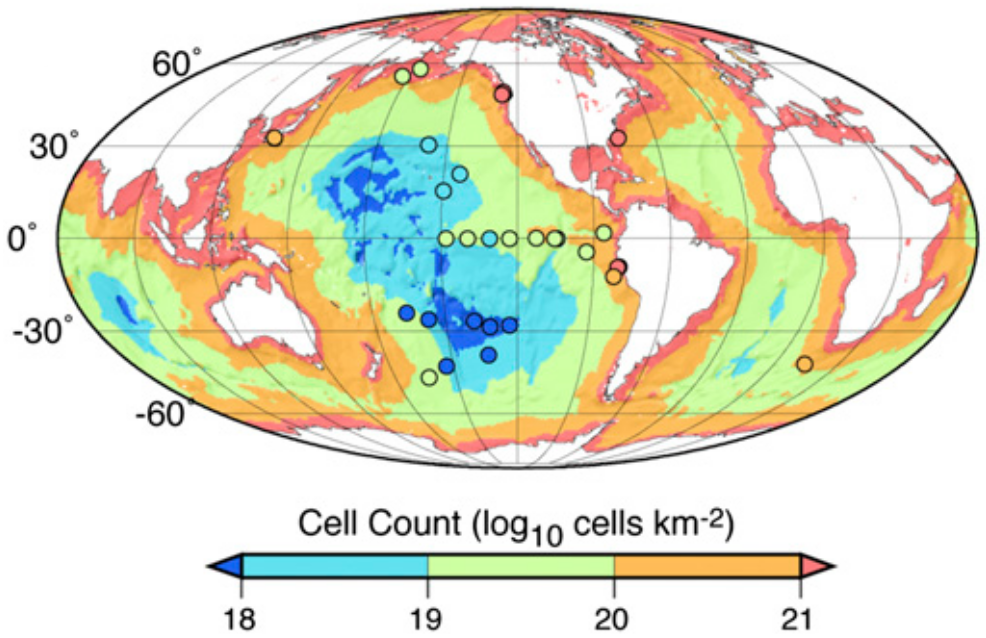
\includegraphics[width=0.7\linewidth]{figures/kallmeyer2012} 

}

\caption{Global distribution of the integrated number of microbial cells in marine sediments. The colours of the dots indicate the number of cells calculated for specific sites. From Kallmeyer et al. (\protect\hyperlink{ref-Kallmeyer2012}{2012}).}\label{fig:kallmeyer2012}
\end{figure}



\hypertarget{section-habitat}{%
\section{Marine sediments: a habitat for microbes}\label{section-habitat}}

Sedimentation of organic matter from the water column serves as the primary source of electron donors and thus energy for microbes in marine sediments (\protect\hyperlink{ref-Jorgensen2019}{Jørgensen et al., 2019}; \protect\hyperlink{ref-Kallmeyer2012}{Kallmeyer et al., 2012}; \protect\hyperlink{ref-Orsi2018}{Orsi, 2018}). This process is influenced by several factors, such as the productivity and depth of the overlying water column, as well as terrestrial input (\protect\hyperlink{ref-Berger1990}{Berger and Wefer, 1990}; \protect\hyperlink{ref-Jahnke1996}{Jahnke, 1996}). High sedimentation rates create anoxic sediments rich in organic matter (\protect\hyperlink{ref-Bowles2014}{Bowles et al., 2014}; \protect\hyperlink{ref-Jorgensen1982}{Jørgensen, 1982}), while low rates enable oxygen to penetrate deeper into the sediment (\protect\hyperlink{ref-DHondt2009}{D'Hondt et al., 2009}; \protect\hyperlink{ref-Roy2012}{Røy et al., 2012}). The sedimentation rate is closely linked to the productivity of the water column, which tends to be higher on the continental shelf compared to the open ocean (\protect\hyperlink{ref-Orsi2018}{Orsi, 2018}). Thus, anoxic conditions in continental shelf sediments develop close to the sediment surface (\protect\hyperlink{ref-Bowles2014}{Bowles et al., 2014}), whereas in the open ocean, where both productivity and sedimentation rates are lower, oxygen-rich zones can extend up to 30 \si{\m} below the sediment surface (\protect\hyperlink{ref-Roy2012}{Røy et al., 2012}).

The composition of the microbial community varies greatly between oxic and anoxic sediments, reflecting the distinct environmental conditions present in these two types of habitats (\protect\hyperlink{ref-Hoshino2020}{Hoshino et al., 2020}; \protect\hyperlink{ref-Orsi2018}{Orsi, 2018}). In oxic sediments, microbial growth is typically limited by the availability of organic matter. In contrast, microbes in anoxic sediments are primarily regulated by the concentrations of terminal electron acceptors, most commonly sulphate. The abundance of microbial cells is markedly greater in anoxic sediments than in their oxic counterparts, with differences reaching up to eight orders of magnitude (\protect\hyperlink{ref-Jorgensen2016}{Jørgensen and Marshall, 2016}; \protect\hyperlink{ref-Kallmeyer2012}{Kallmeyer et al., 2012}). For instance, in coastal anoxic mud, microbial cell counts can be as high as 10\textsuperscript{10} \si{\cellsPerCubiccm}, whereas oxic clay found in deep-sea regions, which is poor in organic matter, averages only about 10\textsuperscript{2} \si{\cellsPerCubiccm} (\protect\hyperlink{ref-Jorgensen2016}{Jørgensen and Marshall, 2016}). Global analyses indicate that in oxic sediments, cell abundance drops below 10\textsuperscript{7} \si{\cellsPerg} just 0.1 \si{\m} beneath the seafloor. In contrast, even at 1 \si{\m} beneath the seafloor in anoxic sediments, the typical concentration of cells ranges from 10\textsuperscript{7} to 10\textsuperscript{9} \si{\cellsPerg} (\protect\hyperlink{ref-Kallmeyer2012}{Kallmeyer et al., 2012}; \protect\hyperlink{ref-Orsi2018}{Orsi, 2018}). The highest microbial abundances have been recorded in the shallow, eutrophic regions of the Baltic Sea, while the central areas of the North and South Pacific Ocean gyres exhibit some of the lowest abundances (\protect\hyperlink{ref-Jorgensen2016}{Jørgensen and Marshall, 2016}). Here, at sediment depths greater than 20 \si{\m}, microbial counts fall below measurable levels (\protect\hyperlink{ref-DHondt2009}{D'Hondt et al., 2009}, \protect\hyperlink{ref-DHondt2015}{2015}; \protect\hyperlink{ref-Roy2012}{Røy et al., 2012}). The exceptionally low abundances observed in deep-sea sediments of the great ocean gyres are attributed to extremely low sedimentation rates. These rates allow deep oxygen penetration and extensive mineralisation of organic matter prior to deeper burial (\protect\hyperlink{ref-DHondt2009}{D'Hondt et al., 2009}, \protect\hyperlink{ref-DHondt2015}{2015}; \protect\hyperlink{ref-Orsi2018}{Orsi, 2018}).

\newpage

Sediments present a challenging environment for microbial survival due to marked changes in environmental conditions throughout the sediment core. Nevertheless, diverse prokaryotic communities have been identified from the sediment surface down to depths of approximately 2.5 \si{\km} (\protect\hyperlink{ref-Inagaki2015}{Inagaki et al., 2015}). The vertical structure of the sediment core reflects the sedimentation of fresh material from the water column to the seabed and its burial over time (\protect\hyperlink{ref-Orsi2018}{Orsi, 2018}; \protect\hyperlink{ref-Petro2017}{Petro et al., 2017}). Microbial cells from the water column or the seabed surface are buried alongside this material, gradually becoming separated from the sediment surface while being subjected to changing environmental conditions (\protect\hyperlink{ref-Petro2017}{Petro et al., 2017}). As sediment age and depth increase, microbes encounter an important challenge: the reduction of available organic matter (\protect\hyperlink{ref-Jorgensen2016}{Jørgensen and Marshall, 2016}; \protect\hyperlink{ref-Petro2017}{Petro et al., 2017}). More labile organic compounds are depleted in shallower sediment layers, leading to impoverished organic matter in older and deeper sediments (\protect\hyperlink{ref-Jorgensen2016}{Jørgensen and Marshall, 2016}; \protect\hyperlink{ref-Middelburg1989}{Middelburg, 1989}; \protect\hyperlink{ref-Petro2017}{Petro et al., 2017}). Consequently, the composition of organic matter shifts towards a higher content of refractory matter, which limits energy sources and results in slower microbial activity in deeper sediment layers (\protect\hyperlink{ref-Jorgensen2016}{Jørgensen and Marshall, 2016}; \protect\hyperlink{ref-Orsi2018}{Orsi, 2018}; \protect\hyperlink{ref-Petro2017}{Petro et al., 2017}). Studies have shown that microbial activity decreases by two to three orders of magnitude in sediment layers just a few meters deep compared to surface sediment (\protect\hyperlink{ref-Petro2017}{Petro et al., 2017}; \protect\hyperlink{ref-Roy2012}{Røy et al., 2012}). Additionally, a corresponding decline in cell abundance and an increase in generation time has been observed at the same depth (\protect\hyperlink{ref-Kallmeyer2012}{Kallmeyer et al., 2012}; \protect\hyperlink{ref-Starnawski2017}{Starnawski et al., 2017}; Figure \ref{fig:starnawski2017}). Microbial activity, cell abundance, and generation time can all be linked to sediment age and the declining availability of organic matter (\protect\hyperlink{ref-Petro2017}{Petro et al., 2017}; \protect\hyperlink{ref-Starnawski2017}{Starnawski et al., 2017}).
\bigskip

\begin{figure}

{\centering 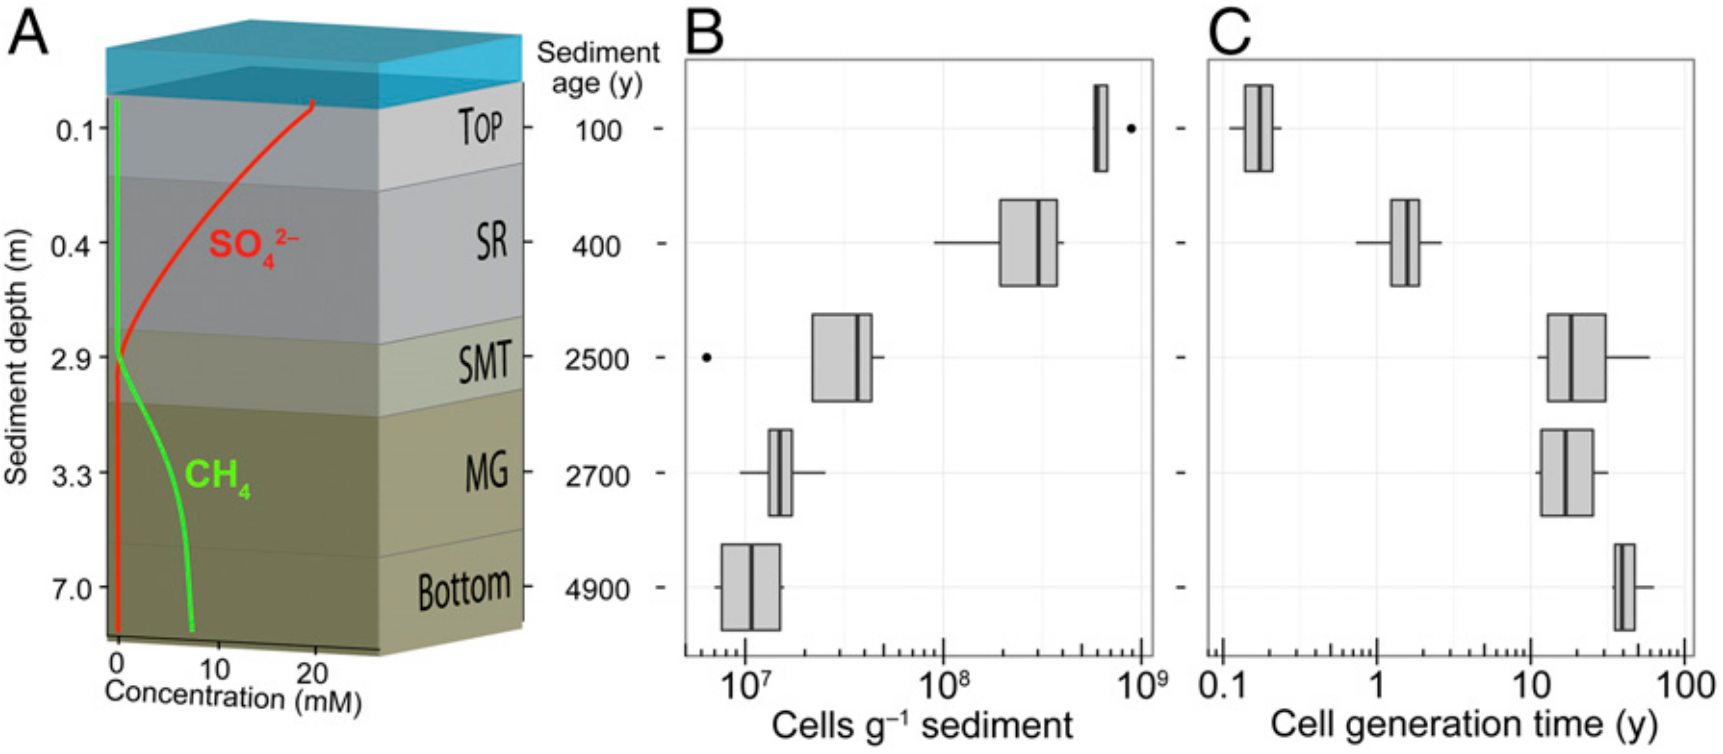
\includegraphics[width=0.95\linewidth]{figures/starnawski2012} 

}

\caption{The vertical biogeochemical zonation (A) and the corresponding distribution of microbial cell abundances (B) and generation times (C) in sediments. Biogeochemical zones: Top, surface sediment; SR, upper sulphate-rich sediment; SMT, sulphate--methane transition zone; MG, methanogenic sediment; Bottom, deep methanogenic zone. From Starnawski et al. (\protect\hyperlink{ref-Starnawski2017}{2017}).}\label{fig:starnawski2017}
\end{figure}



The sediment column is characterised not only by a decline in the availability of organic matter but also by changes in biogeochemical zones as sediment depth increases (\protect\hyperlink{ref-Starnawski2017}{Starnawski et al., 2017}; Figure \ref{fig:starnawski2017}). These changes are accompanied by variations in specific terminal electron acceptors, with each layer identified by the most energetically favourable and available acceptor of organic matter mineralisation (\protect\hyperlink{ref-Canfield1993}{Canfield et al., 1993}; \protect\hyperlink{ref-Froelich1979}{Froelich et al., 1979}; \protect\hyperlink{ref-Thamdrup1994}{Thamdrup et al., 1994}). Starting from the top, the biogeochemical zones include an oxic layer, where oxygen (\ch{O2}) serves as the terminal electron acceptor; a zone of nitrate (\ch{NO3-}) reduction; zones of manganese {[}\ch{Mn({IV})}{]} and iron {[}\ch{Fe({III})}{]} oxides reduction; a zone of sulphate (\ch{SO4^2-}) reduction; and the deepest methanogenic layer, where carbon dioxide (\ch{CO2}) is converted to methane (\ch{CH4}; \protect\hyperlink{ref-Orcutt2011}{Orcutt et al., 2011}). This biogeochemical stratification can be disrupted in the surface layer due to bioturbation (\protect\hyperlink{ref-Kristensen2001}{Kristensen, 2001}), typically extending to a depth of about 10 ± 5 \si{\cm} (\protect\hyperlink{ref-Boudreau1998}{Boudreau, 1998}; \protect\hyperlink{ref-Meysman2006}{Meysman et al., 2006}; \protect\hyperlink{ref-Petro2017}{Petro et al., 2017}). This activity generates a layer of considerable biogeochemical heterogeneity, allowing for localised deeper oxygen penetration (\protect\hyperlink{ref-Boudreau1998}{Boudreau, 1998}; \protect\hyperlink{ref-Meysman2006}{Meysman et al., 2006}). In addition, bioturbation allows for deeper transport of organic matter, which leads to increased microbial activity and dynamics in this layer (\protect\hyperlink{ref-Petro2017}{Petro et al., 2017}). Beneath the bioturbation zone, environmental conditions stabilise, organic matter sources diminish, and diffusion becomes the primary process (\protect\hyperlink{ref-Jorgensen2016}{Jørgensen and Marshall, 2016}; \protect\hyperlink{ref-Petro2017}{Petro et al., 2017}). Here, sulphate reduction is the main process of organic matter mineralisation (\protect\hyperlink{ref-Jorgensen1982}{Jørgensen, 1982}; \protect\hyperlink{ref-Petro2017}{Petro et al., 2017}). This layer is separated from the deeper methanogenic region by a narrow sulphate-methane transition (SMT) zone characterised by sulphate-dependent methane oxidation and by a peak in the sulphate reduction rate (\protect\hyperlink{ref-Leloup2007}{Leloup et al., 2007}; \protect\hyperlink{ref-Petro2017}{Petro et al., 2017}; \protect\hyperlink{ref-Thomsen2001}{Thomsen et al., 2001}). The deeper layers, lacking sulphate, primarily rely on methanogenesis for mineralisation (\protect\hyperlink{ref-Petro2017}{Petro et al., 2017}).

\hypertarget{molecular-techniques-for-studying-sediment-microbial-communities}{%
\section{Molecular techniques for studying sediment microbial communities}\label{molecular-techniques-for-studying-sediment-microbial-communities}}

Traditionally, microbial communities were primarily described through cultivation techniques (\protect\hyperlink{ref-Amann1995}{Amann et al., 1995}). However, it is now well established that less than 1\si{\percent} of microorganisms can be cultured in laboratory settings (\protect\hyperlink{ref-Ferguson1984}{Ferguson et al., 1984}; \protect\hyperlink{ref-Jannasch1959}{Jannasch and Jones, 1959}), a phenomenon preventing the accurate description of microbial populations known as the ``great plate count anomaly'' (\protect\hyperlink{ref-Amann1995}{Amann et al., 1995}; \protect\hyperlink{ref-Staley1985}{Staley and Konopka, 1985}). This discrepancy is attributed to factors such as the selective nature of culture media, the presence of inactive cells, and the aggregation of bacteria (\protect\hyperlink{ref-Jannasch1959}{Jannasch and Jones, 1959}). To address the culture-dependent limitations, Pace et al. (\protect\hyperlink{ref-Pace1986}{1986}) pioneered molecular microbial ecology by cloning DNA extracted from environmental samples and by sequencing the 16S rRNA gene. This innovative approach allowed for the identification of microorganisms without the need for cultivation, enabling studies of microbial ecology based on the molecular phylogeny of the 16S rRNA gene (\protect\hyperlink{ref-Rappe2003}{Rappé and Giovannoni, 2003}; \protect\hyperlink{ref-Woese1990}{Woese et al., 1990}; \protect\hyperlink{ref-Woese1977}{Woese and Fox, 1977}). As a result, many novel taxonomic groups were described (\protect\hyperlink{ref-Okabe2010}{Okabe et al., 2010}). The assessment of microbial communities in coastal marine sediments began with the study by Gray and Herwig (\protect\hyperlink{ref-Gray1996}{1996}), which reported the phylogenetic composition of a bacterial community within marine nearshore sediments. Nowadays, determining the structure of the microbial community typically involves extracting environmental DNA, amplifying a fragment of the 16S rRNA gene using polymerase chain reaction (PCR), and sequencing with various next-generation sequencing (NGS) technologies, usually the Illumina MiSeq platform (\protect\hyperlink{ref-Hoshino2020}{Hoshino et al., 2020}; \protect\hyperlink{ref-Kozich2013}{Kozich et al., 2013}). Although this methodological approach has revolutionised marine microbial ecology, focusing on a single gene or gene fragment allows for the estimation of only the microbial community composition and dynamics. To characterise the potential and active metabolic processes of microbes, a comprehensive identification and quantification of all present genes and their products is essential (\protect\hyperlink{ref-Zhang2010}{W. Zhang et al., 2010}).

A commonly recommended approach to assess the potential metabolic processes carried out by microbes in the environment is metagenomics (\protect\hyperlink{ref-Heidelberg2010}{Heidelberg et al., 2010}). In contrast to traditional genomics, which focuses on the genomic DNA of a single organism, metagenomics explores the collective genomic information of all organisms present in a community (\protect\hyperlink{ref-Quince2017}{Quince et al., 2017}). The typical metagenomic method used in studies is shotgun metagenomics, in which total DNA is isolated from the environmental sample and sequenced in an untargeted (``shotgun'') approach using high-throughput sequencing techniques (\protect\hyperlink{ref-Heidelberg2010}{Heidelberg et al., 2010}; \protect\hyperlink{ref-Quince2017}{Quince et al., 2017}). Usually, total DNA is isolated from the environmental sample and used for metagenomic library preparation and sequencing (\protect\hyperlink{ref-Quince2017}{Quince et al., 2017}). The nucleotide sequences obtained are then assembled into longer sequences, known as contigs, often using bioinformatic tools based on the de Bruijn graph (\protect\hyperlink{ref-Quince2017}{Quince et al., 2017}; \protect\hyperlink{ref-Simpson2015}{Simpson and Pop, 2015}). The assembled reads are then compared with existing databases for taxonomic classification and functional annotation (\protect\hyperlink{ref-Quince2017}{Quince et al., 2017}; \protect\hyperlink{ref-Simon2011}{Simon and Daniel, 2011}). An important advantage of this approach is that it eliminates potential biases associated with amplification of specific DNA fragments by PCR, such as limited primer coverage (\protect\hyperlink{ref-Apprill2015}{Apprill et al., 2015}; \protect\hyperlink{ref-Parada2016}{Parada et al., 2016}; \protect\hyperlink{ref-Simon2011}{Simon and Daniel, 2011}). Indeed, direct sequencing of total DNA has been shown to be the most accurate method for determining taxonomic composition, even though it requires more resources for sequencing and computation (\protect\hyperlink{ref-Simon2011}{Simon and Daniel, 2011}; \protect\hyperlink{ref-vonMering2007}{von Mering et al., 2007}). Metagenomics is now widely used to characterise microbial diversity and metabolic potential in both surface and deep sediments (\protect\hyperlink{ref-Marshall2018}{Marshall et al., 2018}; \protect\hyperlink{ref-Moore2020}{Moore et al., 2020}). However, to comprehensively study the processes carried out by microbial communities, it is essential to integrate other omics approaches that focus on gene products and active processes, such as metaproteomics.

Wilmes and Bond (\protect\hyperlink{ref-Wilmes2004}{2004}) proposed the term ``metaproteomics'' to describe the large-scale characterisation of the entire protein composition of a microbial community at a given time. The methods used to identify these proteins are based on approaches originally developed for proteomic analyses (\protect\hyperlink{ref-VanDenBossche2025}{Van Den Bossche et al., 2025}). These methods typically involve enzymatic digestion of the isolated proteins, usually with trypsin, separation of the peptides using liquid chromatography, and peptide analysis by tandem mass spectrometry (LC-MS/MS; \protect\hyperlink{ref-VanDenBossche2025}{Van Den Bossche et al., 2025}; \protect\hyperlink{ref-Wang2014}{D.-Z. Wang et al., 2014}). A suitable approach for the enzymatic digestion of proteins isolated from environmental samples is filter-aided sample preparation (FASP), which enables the removal of many contaminating compounds that are usually present in environments such as soils and sediments and are often isolated together with proteins (\protect\hyperlink{ref-VanDenBossche2025}{Van Den Bossche et al., 2025}; \protect\hyperlink{ref-Wisniewski2009}{Wiśniewski et al., 2009}). In the final bioinformatic analysis step, the peptide spectra are matched with theoretical spectra from protein sequence databases (\protect\hyperlink{ref-Saito2019}{Saito et al., 2019}; \protect\hyperlink{ref-VanDenBossche2025}{Van Den Bossche et al., 2025}). This process enables both the identification and quantification of peptides and their corresponding proteins (\protect\hyperlink{ref-VanDenBossche2025}{Van Den Bossche et al., 2025}). Determining the full spectrum of proteins produced by microbial communities poses a number of challenges, mainly due to the complexity of metaproteomes (\protect\hyperlink{ref-Wilmes2015}{Wilmes et al., 2015}). For example, the wide range of abundance of proteins in a metaproteomic sample and the low coverage of protein sequence databases pose limitations to successful protein identification (\protect\hyperlink{ref-Saito2019}{Saito et al., 2019}; \protect\hyperlink{ref-Wang2014}{D.-Z. Wang et al., 2014}; \protect\hyperlink{ref-Wilmes2015}{Wilmes et al., 2015}). Despite these obstacles, metaproteomics holds great promise in linking genetic potential to phenotype and thus improving our understanding of the processes carried out by microbial communities (\protect\hyperlink{ref-Wilmes2015}{Wilmes et al., 2015}). In addition, metaproteomic techniques have been successfully applied in various types of marine sediments, e.g.~cold seeps (\protect\hyperlink{ref-Glass2014}{Glass et al., 2014}; \protect\hyperlink{ref-Stokke2012}{Stokke et al., 2012}), diffuse hydrothermal venting (\protect\hyperlink{ref-Urich2014}{Urich et al., 2014}), mudflat aquaculture (\protect\hyperlink{ref-Lin2015}{Lin et al., 2015}), and chronically petroleum-polluted (\protect\hyperlink{ref-Bargiela2015}{Bargiela et al., 2015}) sediments.

\newpage

\hypertarget{section-composition}{%
\section{Composition of sediment microbial communities}\label{section-composition}}

Using the previously described molecular techniques based on 16S rRNA gene sequencing, a comprehensive overview of the taxonomic composition of microbial communities in marine sediments was obtained. Large differences were observed between oxic and anoxic sediments (\protect\hyperlink{ref-Hoshino2020}{Hoshino et al., 2020}; Figure \ref{fig:hoshino2020}), which could be related to the environmental differences that characterise these types of sediments (Section \ref{section-habitat}). The data showed that the proportion of bacteria in marine sediments is generally higher than that of archaea and that the contribution of archaea is more pronounced in low-oxygen sediments than in those with higher oxygen content (\protect\hyperlink{ref-Hoshino2020}{Hoshino et al., 2020}; \protect\hyperlink{ref-Hoshino2019}{Hoshino and Inagaki, 2019}). Within the archaeal community, the phyla \emph{Asgardaeota} and \emph{Crenarchaeota} characterise the anoxic sediments, while the phylum \emph{Thaumarchaeota} dominates in oxic sediments (\protect\hyperlink{ref-Durbin2011}{Durbin and Teske, 2011}; \protect\hyperlink{ref-Hoshino2020}{Hoshino et al., 2020}; \protect\hyperlink{ref-Lauer2016}{Lauer et al., 2016}). Furthermore, within the bacterial community, members of \emph{Atribacteria}, \emph{Chloroflexi}, and \emph{Planctomycetes} are predominant in low-oxygen sediments, while \emph{Alphaproteobacteria}, \emph{Gammaproteobacteria}, and \emph{Firmicutes} dominate in sediments with higher oxygen content (\protect\hyperlink{ref-Durbin2011}{Durbin and Teske, 2011}; \protect\hyperlink{ref-Hoshino2020}{Hoshino et al., 2020}).
\bigskip

\begin{figure}

{\centering 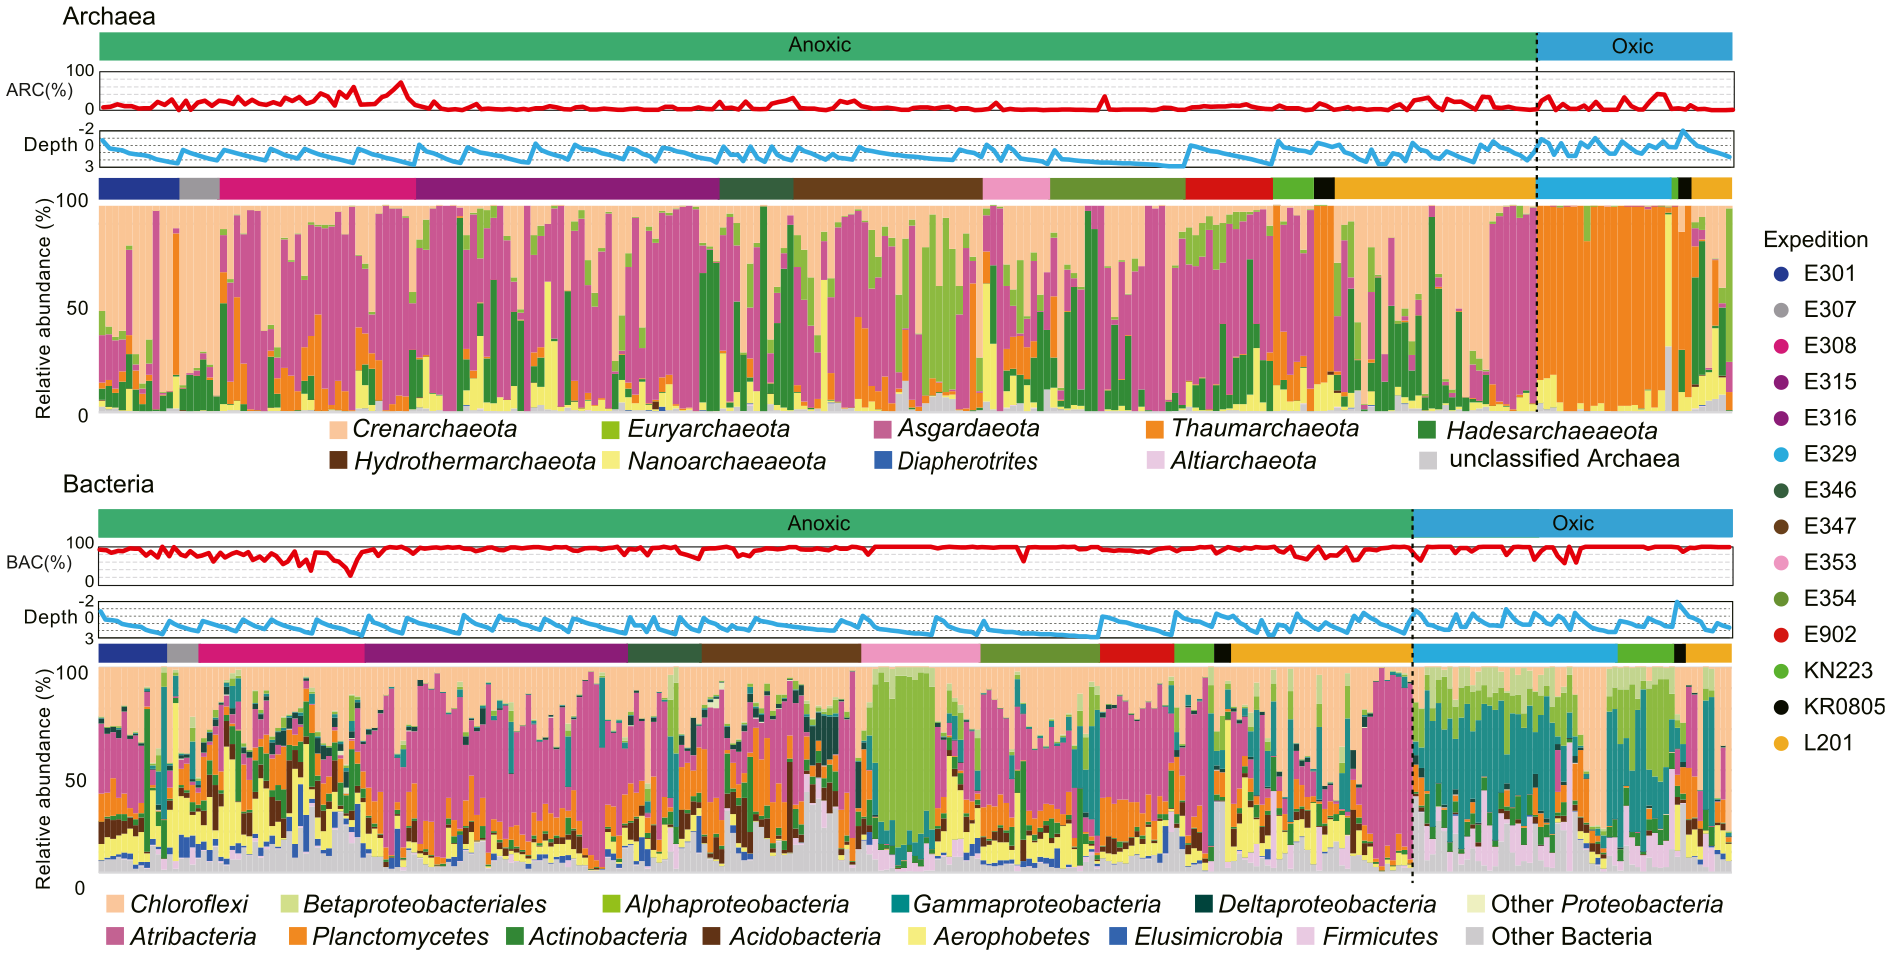
\includegraphics[width=1\linewidth]{figures/hoshino2020} 

}

\caption{Differences in taxonomic composition between microbial communities in oxic and anoxic marine sediments. The composition was determined using universal primers targeting both archaea and bacteria. The relative abundance of archaeal (ARC) and bacterial (BAC) sequences in each sample is represented by a red line, while sediment depth is shown on a logarithmic scale with a light blue line. Sampling expeditions are colour-coded above the corresponding bar. From Hoshino et al. (\protect\hyperlink{ref-Hoshino2020}{2020}).}\label{fig:hoshino2020}
\end{figure}



In addition to the differences between oxic and anoxic sediments, major changes in microbial taxonomic composition and richness are generally observed with increasing sediment depth (\protect\hyperlink{ref-Chen2017}{Chen et al., 2017}; \protect\hyperlink{ref-Hoshino2020}{Hoshino et al., 2020}; \protect\hyperlink{ref-Kirkpatrick2019}{Kirkpatrick et al., 2019}; \protect\hyperlink{ref-Petro2017}{Petro et al., 2017}; \protect\hyperlink{ref-Walsh2016a}{Walsh et al., 2016}). These changes could also be related to shifts in environmental conditions with increasing sediment depth, as in the case of differences between oxic and anoxic sediments (Section \ref{section-habitat}). In general, bacteria dominate over archaea in surface sediments, while their abundance becomes similar with increasing sediment depth (\protect\hyperlink{ref-Chen2017}{Chen et al., 2017}). The higher proportion of archaea in deeper sediments is probably related to their adaptability to limited sources of organic matter (\protect\hyperlink{ref-Hoehler2013}{Hoehler and Jørgensen, 2013}). Interestingly, differences in the change in archaeal and bacterial richness with increasing sediment depth were observed between oxic and anoxic sediments. In anoxic sediments, both bacterial and archaeal richness generally decrease with increasing sediment depth, whereas in oxic sediments, archaeal richness remains stable and only bacterial richness decreases (\protect\hyperlink{ref-Hoshino2020}{Hoshino et al., 2020}). Members of \emph{Gammaproteobacteria}, \emph{Deltaproteobacteria} (reclassified as phylum \emph{Desulfobacterota}), \emph{Alphaproteobacteria}, \emph{Acidobacteria}, and \emph{Bacteroidetes} show higher proportions in surface sediments, while the subsurface is characterised by \emph{Atribacteria}, \emph{Chloroflexi}, and various archaeal groups such as \emph{Bathyarchaeota} and \emph{Lokiarchaeota} (\protect\hyperlink{ref-Chen2017}{Chen et al., 2017}; \protect\hyperlink{ref-Petro2017}{Petro et al., 2017}; \protect\hyperlink{ref-Waite2020}{Waite et al., 2020}; \protect\hyperlink{ref-Walsh2016a}{Walsh et al., 2016}). Interestingly, a clear shift in the taxonomic composition of the bacterial community was observed at a sediment depth of around 1 \si{\km} (\protect\hyperlink{ref-Inagaki2015}{Inagaki et al., 2015}). The phyla \emph{Chloroflexi} and \emph{Atribacteria}, which are characteristic of subsurface sediments, become less present and groups known to dominate terrestrial soil habitats such as \emph{Actinobacteria}, \emph{Proteobacteria}, \emph{Firmicutes}, \emph{Bacteroidetes}, and \emph{Acidobacteria} begin to dominate. These changes were explained by the preservation of indigenous bacteria in terrigenous sediments over tens of millions of years after burial in the seabed (\protect\hyperlink{ref-Inagaki2015}{Inagaki et al., 2015}).

\hypertarget{metabolism-of-sediment-microbial-communities}{%
\section{Metabolism of sediment microbial communities}\label{metabolism-of-sediment-microbial-communities}}

The large differences in environmental conditions between oxic and anoxic sediments as well as throughout the sediment core (Section \ref{section-habitat}) are reflected not only in the composition of the microbial communities (Section \ref{section-composition}), but also in their metabolism (\protect\hyperlink{ref-Orsi2018}{Orsi, 2018}). The sedimentation of organic matter from the water column (\protect\hyperlink{ref-Jorgensen2019}{Jørgensen et al., 2019}; \protect\hyperlink{ref-Kallmeyer2012}{Kallmeyer et al., 2012}; \protect\hyperlink{ref-Orsi2018}{Orsi, 2018}) and the available terminal electron acceptors (\protect\hyperlink{ref-Canfield1993}{Canfield et al., 1993}; \protect\hyperlink{ref-Froelich1979}{Froelich et al., 1979}; \protect\hyperlink{ref-Thamdrup1994}{Thamdrup et al., 1994}) are the main factors influencing the metabolism of these communities (Section \ref{section-habitat}). Studies indicate that in oxic sediments, where organic matter is scarce and the oxygen zone can therefore extend very deep into the sediment, chemolithoautotrophic archaea (e.g.~ammonia-oxidising members of the phylum \emph{Thaumarchaeota}), the ubiquitous gammaproteobacterial JTB255 group, and members of the \emph{Nitrospinae} and \emph{Nitrospirae} perform dark carbon fixation (\protect\hyperlink{ref-Bienhold2016}{Bienhold et al., 2016}; \protect\hyperlink{ref-Dyksma2016}{Dyksma et al., 2016}; \protect\hyperlink{ref-Molari2013}{Molari et al., 2013}; \protect\hyperlink{ref-Orsi2018}{Orsi, 2018}; \protect\hyperlink{ref-Tully2016}{Tully and Heidelberg, 2016}). Furthermore, it appears that ammonia in deep-sea sediments is remineralised from organic compounds by heterotrophic microbes and utilised by ammonia-oxidising \emph{Thaumarchaeota}, highlighting the importance of interactions between different groups of microbes (\protect\hyperlink{ref-Orsi2018}{Orsi, 2018}; \protect\hyperlink{ref-Tully2016}{Tully and Heidelberg, 2016}; \protect\hyperlink{ref-Wankel2015}{Wankel et al., 2015}). The possibility that some members of \emph{Thaumarchaeota} grow mixotrophically further complicates the understanding of the specific roles that each group plays in these habitats (\protect\hyperlink{ref-Qin2014}{Qin et al., 2014}).

In contrast to sediments with high oxygen content, anoxic marine sediments are rich in organic matter, which leads to oxygen consumption in the upper centimetres of the sediment (\protect\hyperlink{ref-Bowles2014}{Bowles et al., 2014}; \protect\hyperlink{ref-Jorgensen2019}{Jørgensen et al., 2019}; \protect\hyperlink{ref-Orsi2018}{Orsi, 2018}; Section \ref{section-habitat}). Below this surface zone, anaerobic microbial metabolism, which relies on the remaining energetically most favourable terminal electron acceptors, is responsible for the mineralisation of organic matter (\protect\hyperlink{ref-Canfield1993}{Canfield et al., 1993}; \protect\hyperlink{ref-Jorgensen2019}{Jørgensen et al., 2019}; \protect\hyperlink{ref-Middelburg2009}{Middelburg and Levin, 2009}; \protect\hyperlink{ref-Orsi2018}{Orsi, 2018}; \protect\hyperlink{ref-Thamdrup1994}{Thamdrup et al., 1994}; Figure \ref{fig:middelburg2009}). Aerobic organisms can mineralise the organic matter completely to carbon dioxide via the tricarboxylic acid cycle. In contrast, the organic matter in anoxic sediments is mineralised in an anaerobic food chain (\protect\hyperlink{ref-Arndt2013}{Arndt et al., 2013}). Degradation begins with the hydrolytic breakdown of high-molecular-weight organic matter such as carbohydrates and proteins by extracellular enzymes, which can be attached to the cell or released into solution (\protect\hyperlink{ref-Arnosti2011}{Arnosti, 2011}; \protect\hyperlink{ref-Jorgensen2019}{Jørgensen et al., 2019}). These complex polymers are converted into substrates that are small enough (typically less than ca. 600 \si{\dalton}, possibly higher for polysaccharides) to be transported across cell membranes (\protect\hyperlink{ref-Arnosti2011}{Arnosti, 2011}; \protect\hyperlink{ref-Jorgensen2019}{Jørgensen et al., 2019}; \protect\hyperlink{ref-Reintjes2017}{Reintjes et al., 2017}). This initial hydrolysis is often the rate-limiting step in the overall degradation of organic matter, emphasising its crucial role in controlling degradation efficiency (\protect\hyperlink{ref-Arndt2013}{Arndt et al., 2013}; \protect\hyperlink{ref-Jorgensen2019}{Jørgensen et al., 2019}). Indeed, research suggests that subsequent mineralisation pathways do not strongly influence degradation rates (\protect\hyperlink{ref-Beulig2018}{Beulig et al., 2018}).

\begin{figure}[ht]

{\centering 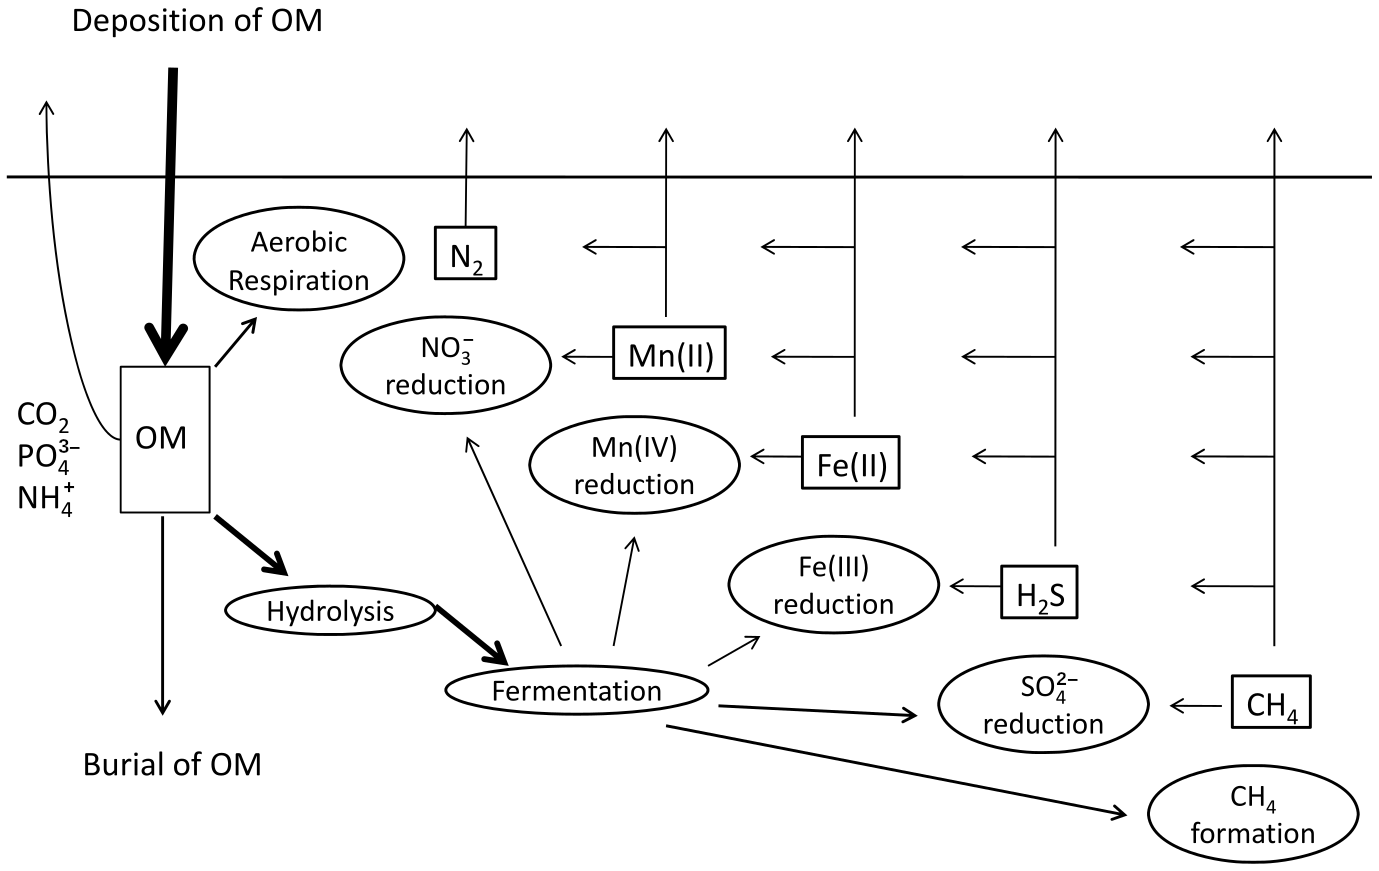
\includegraphics[width=0.9\linewidth]{figures/middelburg2009} 

}

\caption{Conceptual model of the degradation of organic matter in marine sediments. High-molecular-weight organic matter is converted into smaller substrates by hydrolysis and fermentation. These products are respired with the most energetically favourable terminal electron acceptors in the following order of utilisation: oxygen (\ch{O2}), nitrate (\ch{NO3-}), manganese {[}\ch{Mn({IV})}{]} and iron {[}\ch{Fe({III})}{]} oxides, sulphate (\ch{SO4^2-}), and carbon dioxide (\ch{CO2}). Manganese {[}\ch{Mn({II})}{]}, iron {[}\ch{Fe({II})}{]}, sulphide (\ch{H2S + HS- + S^2-}), and methane (\ch{CH4}) are produced and can be oxidised after diffusing upwards. Modified from Middelburg and Levin (\protect\hyperlink{ref-Middelburg2009}{2009}).}\label{fig:middelburg2009}
\end{figure}



The microbial community in the sediment converts small substrates produced by hydrolytic processes such as sugars, amino acids, lipids, organic acids, etc. into a range of products such as short-chain fatty acids (SCFAs; e.g.~formate, acetate, propionate, and butyrate), alcohols, hydrogen, and carbon dioxide through multi-step fermentation processes (\protect\hyperlink{ref-Jorgensen2000}{Jørgensen, 2000}; \protect\hyperlink{ref-Jorgensen2019}{Jørgensen et al., 2019}). \emph{Planctomycetes}, \emph{Anaerolineales} (phylum \emph{Chloroflexi}), and \emph{Bathyarchaeota} have been identified as initial fermenters in anoxic sediments, while \emph{Dehalococcoidia} (phylum \emph{Chloroflexi}), \emph{Deltaproteobacteria} (reclassified as phylum \emph{Desulfobacterota}), and \emph{Nanoarchaeota} may be involved in secondary fermentation (\protect\hyperlink{ref-Suominen2021}{Suominen et al., 2021}; \protect\hyperlink{ref-Waite2020}{Waite et al., 2020}). Since sulphate-reducing microbes are generally unable to utilise the products of hydrolysis of complex organic matter, they take up the substrates produced by the fermenters and respire them to carbon dioxide using sulphate as a terminal electron acceptor (\protect\hyperlink{ref-Jorgensen2000}{Jørgensen, 2000}; \protect\hyperlink{ref-Jorgensen2019}{Jørgensen et al., 2019}). The importance of sulphate reduction is reflected in the estimate that this process in coastal sediments could be responsible for 50\si{\percent} of the mineralisation of organic carbon in the sediment column (\protect\hyperlink{ref-Jorgensen1982}{Jørgensen, 1982}; \protect\hyperlink{ref-Jorgensen2019}{Jørgensen et al., 2019}). The sulphate reducers found in marine sediments belong mainly to uncultured groups within the \emph{Deltaproteobacteria} (reclassified as phylum \emph{Desulfobacterota}), which are only distantly related to cultured sulphate reducers (\protect\hyperlink{ref-Jorgensen2019}{Jørgensen et al., 2019}; \protect\hyperlink{ref-Waite2020}{Waite et al., 2020}). When the sulphate is depleted, the terminal degradation of organic carbon is taken over by methanogenic archaea, whose substrate spectrum is narrower and largely limited to hydrogen, carbon dioxide, and possibly acetate (\protect\hyperlink{ref-Jorgensen2000}{Jørgensen, 2000}; \protect\hyperlink{ref-Jorgensen2019}{Jørgensen et al., 2019}; \protect\hyperlink{ref-Petro2017}{Petro et al., 2017}). Most of the methane produced in the continental shelf and slope sediments diffuses upwards into the SMT zone, where it is oxidised by the anaerobic methanotrophic archaea (ANME), with sulphate serving as a terminal electron acceptor (\protect\hyperlink{ref-Egger2018}{Egger et al., 2018}; \protect\hyperlink{ref-Jorgensen2019}{Jørgensen et al., 2019}).

\hypertarget{section-seagrasses}{%
\section{Seagrasses}\label{section-seagrasses}}

Seagrasses are a polyphyletic group of monocotyledonous angiosperms adapted to a fully submerged lifestyle in marine waters (\protect\hyperlink{ref-Les1997}{Les et al., 1997}; \protect\hyperlink{ref-Orth2006}{Orth et al., 2006}). It is estimated that they evolved from their terrestrial ancestors around 70 to 100 million years ago (\protect\hyperlink{ref-Capo-Bauca2022}{Capó-Bauçà et al., 2022}; \protect\hyperlink{ref-Orth2006}{Orth et al., 2006}; \protect\hyperlink{ref-Wissler2011}{Wissler et al., 2011}). Colonisation of marine habitats is considered a difficult adaptive obstacle, requiring the acquisition of salinity tolerance, underwater vegetative growth, a sufficient anchoring system to withstand wave action and tidal currents, and hydrophilous (water-mediated) pollination (\protect\hyperlink{ref-Arber1920}{Arber, 1920}). Indeed, seagrasses fulfil all four of these characteristics necessary for plants to thrive in the marine environment (\protect\hyperlink{ref-denHartog1970}{den Hartog, 1970}). Moreover, the occurrence of three independent seagrass lineages (Hydrocharitaceae, Cymodoceaceae complex, and Zosteraceae) proves that the acquisition of these traits occurred multiple times and represents an impressive example of convergent evolution in angiosperms (\protect\hyperlink{ref-Les1997}{Les et al., 1997}). There are approximately 70 species regarded as seagrasses, all of which are classified in the order Alismatales (\protect\hyperlink{ref-Short2011}{Short et al., 2011}; \protect\hyperlink{ref-Unsworth2022}{Unsworth et al., 2022}). Within this order, three families consist exclusively of seagrasses, Zosteraceae (three genera), Cymodoceaceae (five genera), and Posidoniaceae (one genus), while the family Hydrocharitaceae contains three genera that are considered seagrasses and 14 genera that are restricted to freshwater habitats (\protect\hyperlink{ref-denHartog2006}{den Hartog and Kuo, 2006}). In addition to the species within these genera, many species of the genus \emph{Ruppia} are sometimes considered seagrasses, while species of the genera \emph{Potamogeton} and \emph{Lepilaena} are considered associates of seagrasses or facultative members of the seagrass community (\protect\hyperlink{ref-Green2003}{Green and Short, 2003}).

% Set page orientation to landscape after the current page is completed
% (\afterpage enables the paragraph to continue after the landscape page)
\afterpage{
    
    % Begin landscape orientation
    \begin{landscape}
    

\begin{figure}[p]

{\centering 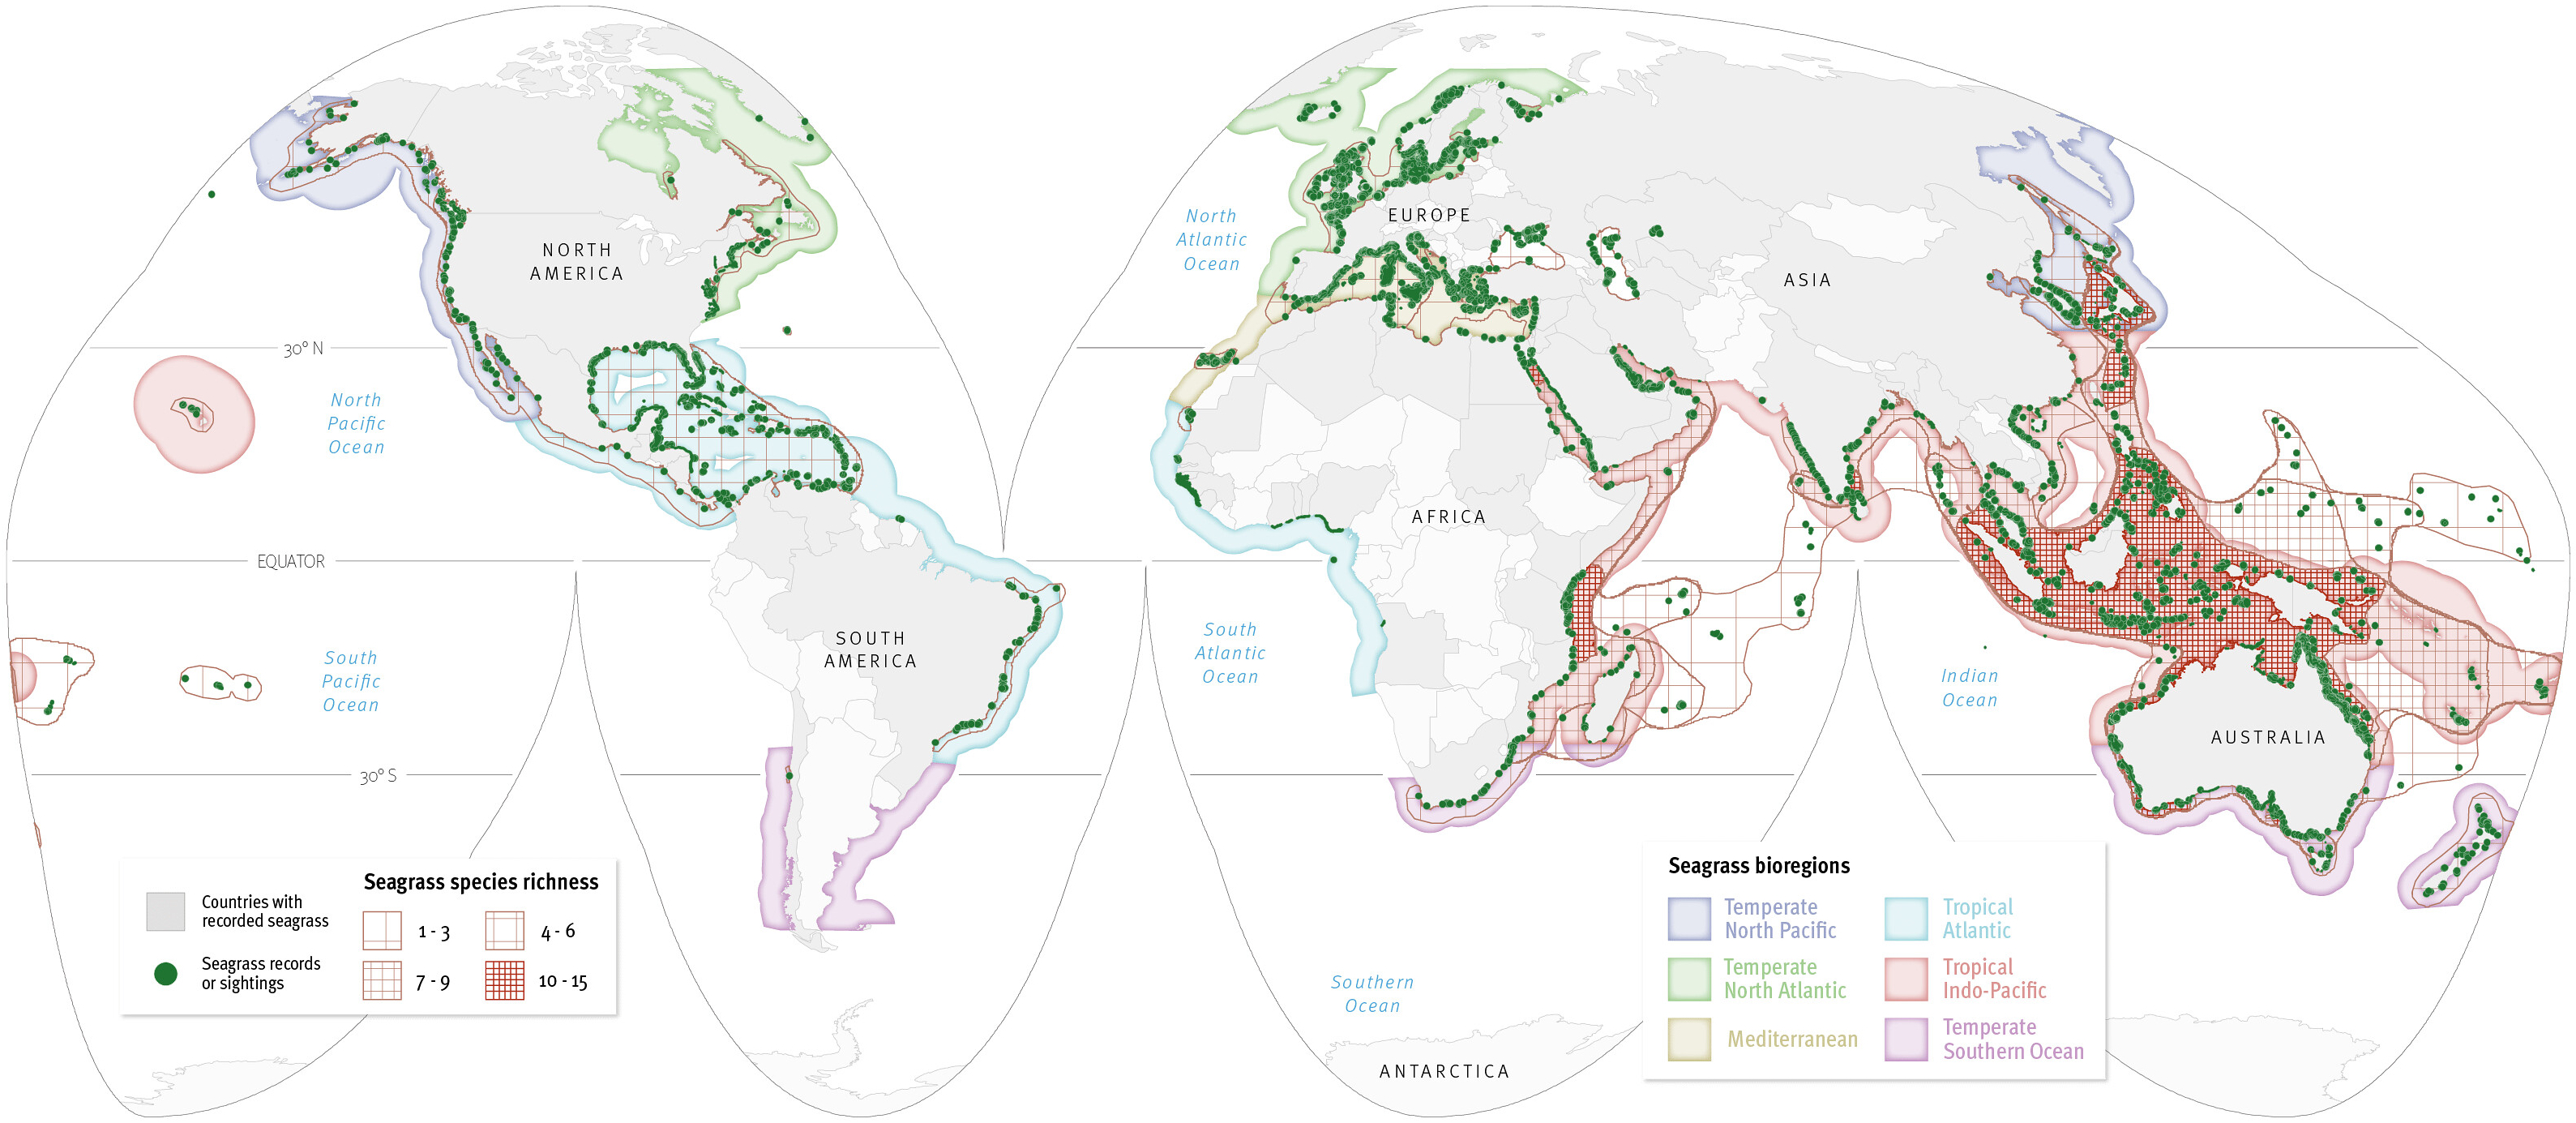
\includegraphics[width=1\linewidth]{figures/westerveld2019} 

}

\caption{Global distribution of seagrasses, species richness, and bioregions. Data sources: Short et al. (\protect\hyperlink{ref-Short2007}{2007}) and UNEP-WCMC and Short (\protect\hyperlink{ref-UnitedNationsEnvironmentProgrammeWorldConservationMonitoringCentreUNEP-WCMC2018}{2018}). Map created by Levi Westerveld/GRID-Arendal (2019) using the Goode homolosine projection (\url{https://grida.no/resources/13590}). From UNEP (\protect\hyperlink{ref-UnitedNationsEnvironmentProgrammeUNEP2020}{2020}).}\label{fig:westerveld2019}
\end{figure}



    
    % End landscape orientation
    \end{landscape}
    
}

Seagrasses occur in shallow marine and estuarine environments of all continents except Antarctica (\protect\hyperlink{ref-denHartog2006}{den Hartog and Kuo, 2006}; \protect\hyperlink{ref-Green2003}{Green and Short, 2003}). The areas containing the highest number of seagrass species are insular South-East Asia, including northern tropical Australia and the Great Barrier Reef, south-eastern India, eastern Africa, southern Japan, and south-western Australia (\protect\hyperlink{ref-Short2007}{Short et al., 2007}; UNEP-WCMC and Short, \protect\hyperlink{ref-UnitedNationsEnvironmentProgrammeWorldConservationMonitoringCentreUNEP-WCMC2018}{2018}; Figure \ref{fig:westerveld2019}). In the Mediterranean Sea, there is a unique temperate--tropical mix of seagrass species (\protect\hyperlink{ref-Short2007}{Short et al., 2007}). \emph{Zostera marina} Linnaeus and \emph{Nanozostera noltei} (Hornemann) Tomlinson et Posluszny, two species common in temperate regions, occur here alongside the endemic \emph{Posidonia oceanica} (Linnaeus) Delile (\protect\hyperlink{ref-Green2003}{Green and Short, 2003}; \protect\hyperlink{ref-Guiry2025}{Guiry and Guiry, 2025}; \protect\hyperlink{ref-Short2007}{Short et al., 2007}). In addition to these species, the Mediterranean is also inhabited by \emph{Halophila stipulacea} (Forsskål) Ascherson, an invasive species thought to have been introduced from the Red Sea through the Suez Canal (Lessepsian migration), and by \emph{Cymodocea nodosa} (Ucria) Ascherson, a seagrass whose congeners inhabit the tropical Indo-Pacific (\protect\hyperlink{ref-Fritsch1895}{Fritsch, 1895}; \protect\hyperlink{ref-Green2003}{Green and Short, 2003}; \protect\hyperlink{ref-Guiry2025}{Guiry and Guiry, 2025}; \protect\hyperlink{ref-Short2007}{Short et al., 2007}). In addition, \emph{Ruppia} spp. have been found in the Mediterranean Sea, but their distribution is generally restricted to shallow waters characterised by fine sediments and strong salinity fluctuations, such as coastal lagoons and brackish habitats (\protect\hyperlink{ref-Green2003}{Green and Short, 2003}; \protect\hyperlink{ref-Mannino2015}{Mannino et al., 2015}). These seagrass species, which are characteristic of the Mediterranean, have also been found in the Adriatic Sea (\protect\hyperlink{ref-Curiel2021}{Curiel et al., 2021}; \protect\hyperlink{ref-Green2003}{Green and Short, 2003}; \protect\hyperlink{ref-Guidetti2002}{Guidetti et al., 2002}).

The seagrass \emph{C. nodosa}, whose sediment microbes are the subject of this doctoral thesis, is, as already mentioned, widespread in the Mediterranean (\protect\hyperlink{ref-Green2003}{Green and Short, 2003}; \protect\hyperlink{ref-Short2007}{Short et al., 2007}). However, it is not restricted to this area. Its range also includes the Atlantic coast of Africa, including the Canary Islands. Here, the southern limit of distribution is south of the Tropic of Cancer (\protect\hyperlink{ref-denHartog1970}{den Hartog, 1970}; \protect\hyperlink{ref-Green2003}{Green and Short, 2003}; \protect\hyperlink{ref-Short2007}{Short et al., 2007}). On the European Atlantic coast, it is also found in Portugal, where it is mixed with temperate seagrasses (\protect\hyperlink{ref-Short2007}{Short et al., 2007}), and in southern Spain (\protect\hyperlink{ref-denHartog1970}{den Hartog, 1970}). In the Adriatic Sea, \emph{C. nodosa} is common in both the northern (\protect\hyperlink{ref-Agostini2003}{Agostini et al., 2003}; \protect\hyperlink{ref-Najdek2020a}{Najdek et al., 2020}; \protect\hyperlink{ref-Orlando-Bonaca2015}{Orlando-Bonaca et al., 2015}; \protect\hyperlink{ref-Smith2025}{S. M. Smith et al., 2025}; \protect\hyperlink{ref-Zavodnik1998}{Zavodnik et al., 1998}) and southern (\protect\hyperlink{ref-denHartog1970}{den Hartog, 1970}; \protect\hyperlink{ref-Macic2014}{Mačić, 2014}) parts of this area of the Mediterranean Sea. This seagrass is generally found in shallow waters, but can sometimes reach a depth of 30 to 40 \si{\m}. The meadows in shallow and deep waters are typically discontinuous (\protect\hyperlink{ref-Green2003}{Green and Short, 2003}). \emph{C. nodosa} is usually found in sheltered locations, such as bays and coastal lagoons (\protect\hyperlink{ref-Agostini2003}{Agostini et al., 2003}; \protect\hyperlink{ref-Green2003}{Green and Short, 2003}; \protect\hyperlink{ref-Najdek2020a}{Najdek et al., 2020}; \protect\hyperlink{ref-Orlando-Bonaca2015}{Orlando-Bonaca et al., 2015}; \protect\hyperlink{ref-Smith2025}{S. M. Smith et al., 2025}; \protect\hyperlink{ref-Zavodnik1998}{Zavodnik et al., 1998}). In general, it is considered a pioneer species that often precedes \emph{P. oceanica} in succession, with which it cannot compete (\protect\hyperlink{ref-denHartog1970}{den Hartog, 1970}; \protect\hyperlink{ref-Green2003}{Green and Short, 2003}). The growth pattern is unimodal, with a biomass maximum in summer, a minimum in winter, and a particularly active growth phase in spring (\protect\hyperlink{ref-Agostini2003}{Agostini et al., 2003}; \protect\hyperlink{ref-Cancemi2002}{Cancemi et al., 2002}; \protect\hyperlink{ref-Najdek2020a}{Najdek et al., 2020}; \protect\hyperlink{ref-Terrados1992}{Terrados and Ros, 1992}; \protect\hyperlink{ref-Zavodnik1998}{Zavodnik et al., 1998}). \emph{C. nodosa} is a dioecious species (\protect\hyperlink{ref-denHartog1970}{den Hartog, 1970}; \protect\hyperlink{ref-Green2003}{Green and Short, 2003}). Flowering has been described in spring and summer, while fruits have been collected from spring to late autumn (\protect\hyperlink{ref-denHartog1970}{den Hartog, 1970}; \protect\hyperlink{ref-Reyes1995}{Reyes et al., 1995}).

\begin{figure}

{\centering 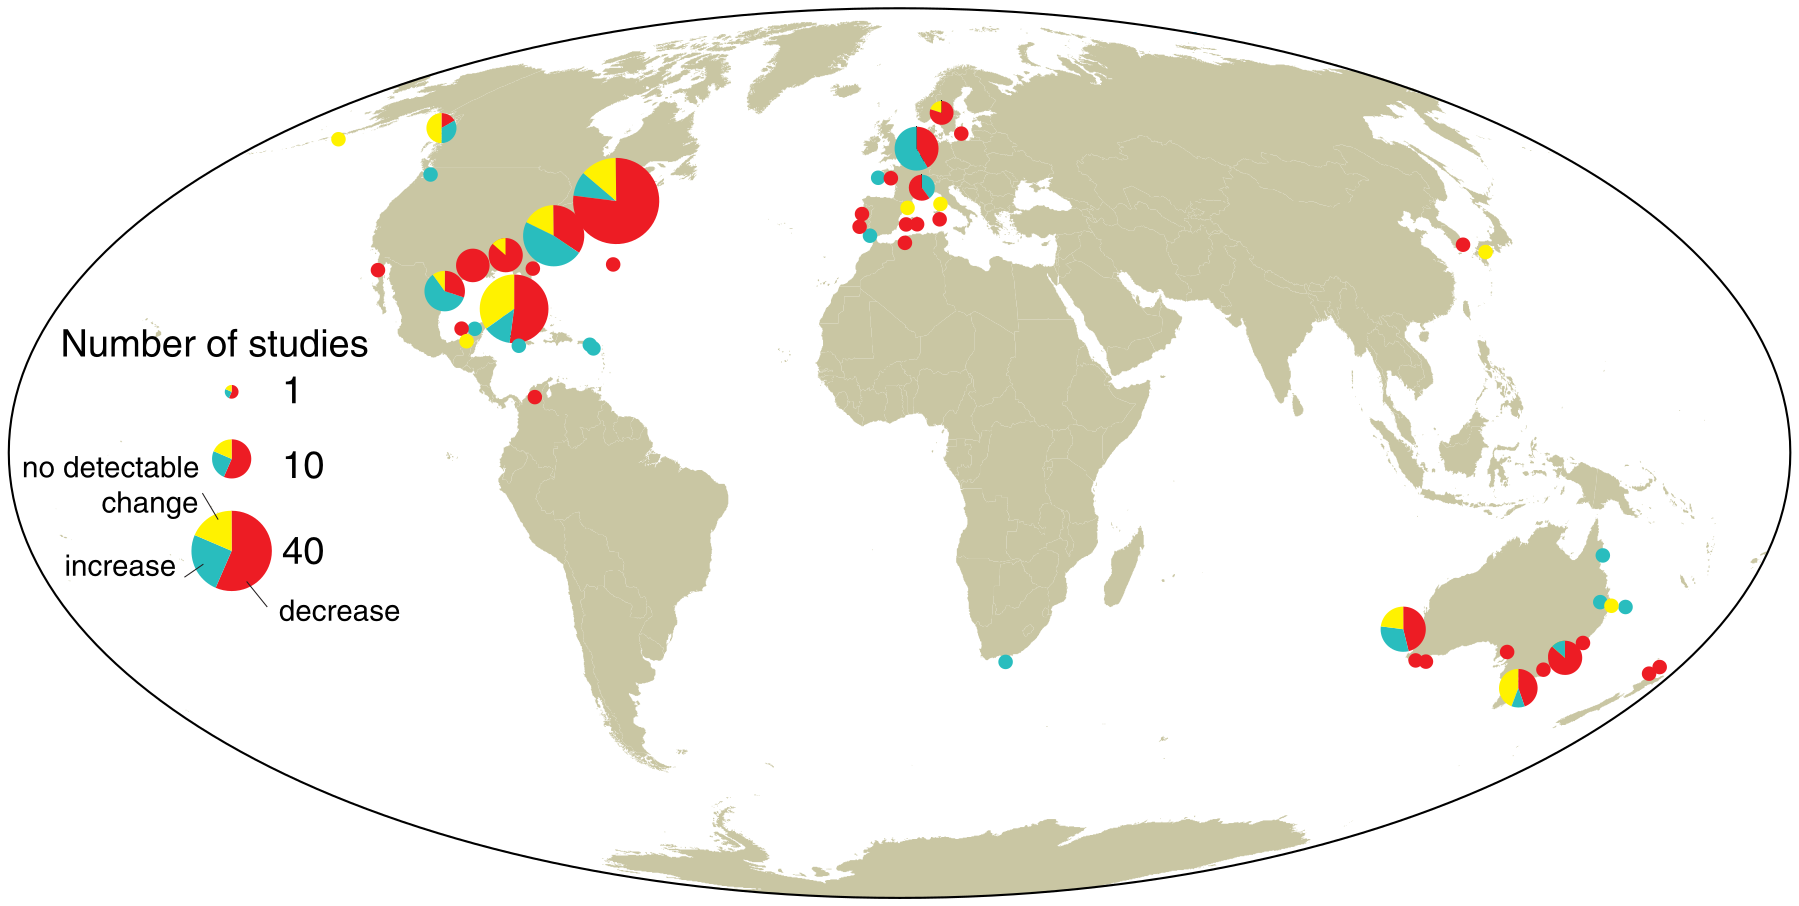
\includegraphics[width=0.9\linewidth]{figures/waycott2009} 

}

\caption{Global assessment of seagrass loss in different coastal areas based on data from 215 sites. An increase or decrease in seagrass area at each site of more than 10\si{\percent} is marked in green and red, respectively. If the final area is within ±10\si{\percent} of the initial area, the change is considered undetectable and marked in yellow. From Waycott et al. (\protect\hyperlink{ref-Waycott2009}{2009}).}\label{fig:waycott2009}
\end{figure}



Seagrasses are considered ecosystem engineers because they cause physical state changes in biotic and abiotic materials and thus modify, maintain, and create habitats (\protect\hyperlink{ref-Jones1994}{C. G. Jones et al., 1994}; \protect\hyperlink{ref-Orth2006}{Orth et al., 2006}). These environments, known as seagrass meadows, are ecologically important because they provide habitat and food for many animals, serve as nursery areas for the larger ocean, attenuate wave energy, stabilise the sediment, and improve the transparency of the water by trapping sediment particles (\protect\hyperlink{ref-Duarte2002}{Duarte, 2002}; \protect\hyperlink{ref-Green2003}{Green and Short, 2003}; \protect\hyperlink{ref-Heck2006}{Heck and Valentine, 2006}). In addition, the sediments of seagrass meadows are enriched with organic carbon through the trapping of organic particles from the water column, the release of dissolved organic carbon by seagrass roots, and the already mentioned stabilisation of the sediment (\protect\hyperlink{ref-Duarte2005}{Duarte, Holmer, et al., 2005}; \protect\hyperlink{ref-Terrados2000}{Terrados and Duarte, 2000}; \protect\hyperlink{ref-vanKatwijk2010}{van Katwijk et al., 2010}). Moreover, the decomposition of seagrass leaves, roots, and rhizomes increases the availability of organic matter in seagrass meadows (\protect\hyperlink{ref-Liu2017}{Liu et al., 2017}; \protect\hyperlink{ref-Peduzzi1991}{Peduzzi and Herndl, 1991}; \protect\hyperlink{ref-Trevathan-Tackett2020}{Trevathan-Tackett et al., 2020}). It is therefore not surprising that the sediments of seagrass meadows are natural hotspots for carbon sequestration. It is estimated that these areas are responsible for up to 20\si{\percent} of global carbon sequestration in marine sediments, although they occupy only 0.1\si{\percent} of the seafloor (\protect\hyperlink{ref-Duarte2005a}{Duarte, Middelburg, et al., 2005}; \protect\hyperlink{ref-Duarte2013}{Duarte et al., 2013}; \protect\hyperlink{ref-Kennedy2010}{Kennedy et al., 2010}). Due to the importance of seagrass meadows, their observed loss on a global scale is worrying (\protect\hyperlink{ref-Dunic2021}{Dunic et al., 2021}; \protect\hyperlink{ref-Orth2006}{Orth et al., 2006}). The area covered by seagrass meadows has declined by 29\si{\percent} worldwide since the end of the 19th century (\protect\hyperlink{ref-Waycott2009}{Waycott et al., 2009}; Figure \ref{fig:waycott2009}). Although more recent estimates have reduced the global loss over the same period to 19\si{\percent}, this is still considerable and the decline continues (\protect\hyperlink{ref-Dunic2021}{Dunic et al., 2021}). The loss of seagrass meadows has also been observed in the Mediterranean (\protect\hyperlink{ref-delosSantos2019}{de los Santos et al., 2019}; \protect\hyperlink{ref-Dunic2021}{Dunic et al., 2021}). In fact, together with the Tropical Atlantic, the Mediterranean experienced the greatest loss of seagrass meadows in absolute numbers, with the decline being greatest from the 1940s to the 1980s and the situation remaining stable thereafter (\protect\hyperlink{ref-Dunic2021}{Dunic et al., 2021}). A partially similar trend in the loss of seagrass meadows was also observed in the Adriatic Sea. After a sharp decline in the 1970s and 1980s, seagrass meadows experienced a phase of recovery in the 1990s. However, from 2007 to 2013 a further loss of seagrass meadows was recorded (\protect\hyperlink{ref-Danovaro2020}{Danovaro et al., 2020}). Although Short et al. (\protect\hyperlink{ref-Short2011}{2011}) estimated a stable population trend for \emph{C. nodosa}, a more recent study using ecological niche modelling predicts, in the worst-case scenario, a sharp decline in suitable habitats for this species due to climate change (\protect\hyperlink{ref-Chefaoui2018}{Chefaoui et al., 2018}). Indeed, several studies reported the decline of \emph{C. nodosa} meadows in different parts of the Mediterranean (\protect\hyperlink{ref-Barsanti2007}{Barsanti et al., 2007}; \protect\hyperlink{ref-Boudouresque2009}{Boudouresque et al., 2009}; \protect\hyperlink{ref-Perez-Ruzafa2006}{Pérez-Ruzafa et al., 2006}; \protect\hyperlink{ref-Shili2002}{Shili et al., 2002}), including the Adriatic Sea (\protect\hyperlink{ref-Green2003}{Green and Short, 2003}; \protect\hyperlink{ref-Orlando-Bonaca2015}{Orlando-Bonaca et al., 2015}, \protect\hyperlink{ref-Orlando-Bonaca2019}{2019}).

\hypertarget{microbial-communities-in-sediments-of-seagrass-meadows}{%
\section{Microbial communities in sediments of seagrass meadows}\label{microbial-communities-in-sediments-of-seagrass-meadows}}

Sediments of seagrass meadows are considered hotspots for microbial activity because, as already mentioned, these habitats are enriched with organic matter directly by seagrasses or through various seagrass-mediated processes (\protect\hyperlink{ref-Duarte2005}{Duarte, Holmer, et al., 2005}; Section \ref{section-seagrasses}). Consequently, studies have shown that microbial abundance, activity, and metabolic diversity are higher in seagrass-vegetated than in nonvegetated sediments (\protect\hyperlink{ref-Delille1996}{Delille et al., 1996}; \protect\hyperlink{ref-Duarte2005}{Duarte, Holmer, et al., 2005}; \protect\hyperlink{ref-Holmer1997}{Holmer and Nielsen, 1997}; \protect\hyperlink{ref-Mohapatra2022}{Mohapatra et al., 2022}; \protect\hyperlink{ref-Smith2004}{A. Smith et al., 2004}). The high organic matter content of seagrass sediments appears to stimulate the proliferation of sulphate-reducing bacteria, which in turn play an important role in the remineralisation of nutrients in these habitats (\protect\hyperlink{ref-Blackburn1994}{Blackburn et al., 1994}; \protect\hyperlink{ref-Duarte2005}{Duarte, Holmer, et al., 2005}; \protect\hyperlink{ref-Holmer1997}{Holmer and Nielsen, 1997}; \protect\hyperlink{ref-Smith2004}{A. Smith et al., 2004}). This is consistent with the already recognised importance of sulphate reduction in the mineralisation of organic carbon in coastal sediments (\protect\hyperlink{ref-Jorgensen1982}{Jørgensen, 1982}; \protect\hyperlink{ref-Jorgensen2019}{Jørgensen et al., 2019}). In addition, the facilitated release and transformation of nutrients by microbes during remineralisation supports seagrass growth and photosynthesis (\protect\hyperlink{ref-Duarte2005}{Duarte, Holmer, et al., 2005}). However, high rates of sulphate reduction can lead to the accumulation of hydrogen sulphide (\ch{H2S}), a potent phytotoxin (\protect\hyperlink{ref-Duarte2005}{Duarte, Holmer, et al., 2005}; \protect\hyperlink{ref-Holmer2001a}{Holmer and Bondgaard, 2001}; \protect\hyperlink{ref-Koch2001}{Koch and Erskine, 2001}), which has been linked to die-off events of seagrass meadows (\protect\hyperlink{ref-Borum2005}{Borum et al., 2005}; \protect\hyperlink{ref-Carlson1994}{Carlson et al., 1994}). The diffusion of oxygen from seagrass roots and the reoxidation of hydrogen sulphide back to sulphate has been recognised as a coping mechanism of seagrasses against hydrogen sulphide toxicity (\protect\hyperlink{ref-Duarte2005}{Duarte, Holmer, et al., 2005}; \protect\hyperlink{ref-Hasler-Sheetal2015}{Hasler-Sheetal and Holmer, 2015}; \protect\hyperlink{ref-Holmer2005}{Holmer et al., 2005}; \protect\hyperlink{ref-Pedersen2004}{Pedersen et al., 2004}). These examples show that seagrasses and sediment microbes live in a state of delicate balance. For the growth and development of seagrasses, it is important that the positive, mutualistic effects of the microbes, such as the remineralisation of nutrients, overcome the negative ones, such as the production of hydrogen sulphide (\protect\hyperlink{ref-Duarte2005}{Duarte, Holmer, et al., 2005}).
\bigskip

The composition of microbial communities living in sediments colonised by seagrasses is not as well studied, as research has mainly focused on the rhizosphere and only occasionally sediment communities have been used for comparison. It has been shown that communities in the rhizosphere are not species-specific and differ from those in the sediment (\protect\hyperlink{ref-Cucio2016}{Cúcio et al., 2016}; \protect\hyperlink{ref-Ettinger2017}{Ettinger et al., 2017}; \protect\hyperlink{ref-Rabbani2021}{Rabbani et al., 2021}; \protect\hyperlink{ref-Zhang2020}{X. Zhang et al., 2020}). One of the most important differences observed is the higher proportion of \emph{Deltaproteobacteria} (reclassified as phylum \emph{Desulfobacterota}) in the bulk sediment, a group that contains many sulphate reducers from marine sediments (\protect\hyperlink{ref-Ettinger2017}{Ettinger et al., 2017}; \protect\hyperlink{ref-Waite2020}{Waite et al., 2020}). In contrast, the rhizosphere is characterised by members of the \emph{Epsilonproteobacteria} (reclassified as phylum \emph{Campylobacterota}; \protect\hyperlink{ref-Ettinger2017}{Ettinger et al., 2017}; \protect\hyperlink{ref-Jensen2007}{Jensen et al., 2007}; \protect\hyperlink{ref-Waite2017}{Waite et al., 2017}, \protect\hyperlink{ref-Waite2018}{2018}). Microbial communities in sediments colonised by many seagrass species such as \emph{Enhalus acoroides} (Linnaeus f.) Royle, \emph{Thalassia hemprichii} (Ehrenberg) Ascherson (\protect\hyperlink{ref-Liu2018}{Liu et al., 2018}), \emph{Thalassia testudinum} K. D. Koenig (\protect\hyperlink{ref-Ugarelli2024}{Ugarelli et al., 2024}), \emph{Amphibolis antarctica} (Labillardière) Ascherson, \emph{Halodule uninervis} (Forsskål) Ascherson (\protect\hyperlink{ref-Fraser2018}{Fraser et al., 2018}), \emph{Halodule wrightii} Ascherson (\protect\hyperlink{ref-Smith2004}{A. Smith et al., 2004}), \emph{Posidonia oceanica} (\protect\hyperlink{ref-Garcia-Martinez2009}{García-Martínez et al., 2009}), \emph{Nanozostera japonica} (Ascherson et Graebner) Tomlinson et Posluszny, and \emph{Zostera marina} (\protect\hyperlink{ref-Sun2020}{Sun et al., 2020}) have been described (\protect\hyperlink{ref-Guiry2025}{Guiry and Guiry, 2025}). Studies have often found differences between seagrass-vegetated and nonvegetated areas (\protect\hyperlink{ref-Alsaffar2020}{Alsaffar et al., 2020}; \protect\hyperlink{ref-Smith2004}{A. Smith et al., 2004}; \protect\hyperlink{ref-Sun2020}{Sun et al., 2020}; \protect\hyperlink{ref-Zheng2019}{Zheng et al., 2019}). Furthermore, differences in microbial communities have been described even between the periphery and the central region of the seagrass meadow (\protect\hyperlink{ref-Ettinger2017}{Ettinger et al., 2017}). One of the differences between seagrass-vegetated and nonvegetated areas is the higher abundance of archaea in seagrass-colonised sediments (\protect\hyperlink{ref-Zheng2019}{Zheng et al., 2019}). The archaeal community in seagrass sediments generally includes \emph{Crenarchaeota}, \emph{Euryarchaeota}, \emph{Asgardaeota}, \emph{Woesearchaeota}, \emph{Bathyarchaeota}, and \emph{Thaumarchaeota} (\protect\hyperlink{ref-Sun2020}{Sun et al., 2020}; \protect\hyperlink{ref-Zheng2019}{Zheng et al., 2019}), while the bacterial community consists predominantly of \emph{Proteobacteria}, \emph{Chloroflexi}, \emph{Planctomycetes}, \emph{Bacteroidetes}, \emph{Acidobacteria}, \emph{Epsilonproteobacteria} (reclassified as phylum \emph{Campylobacterota}), and \emph{Latescibacteria} (\protect\hyperlink{ref-Sun2020}{Sun et al., 2020}; \protect\hyperlink{ref-Waite2017}{Waite et al., 2017}, \protect\hyperlink{ref-Waite2018}{2018}).

\hypertarget{chapter-objectives-and-hypotheses}{%
\chapter{OBJECTIVES AND HYPOTHESES}\label{chapter-objectives-and-hypotheses}}

Seagrasses are considered ecosystem engineers because they modify, maintain, and create habitats (\protect\hyperlink{ref-Jones1994}{C. G. Jones et al., 1994}; \protect\hyperlink{ref-Orth2006}{Orth et al., 2006}). The decline and loss of seagrass meadows, which are ecologically important habitats, is worrying as it has been observed on a global scale, including in the Mediterranean and Adriatic Sea (\protect\hyperlink{ref-Danovaro2020}{Danovaro et al., 2020}; \protect\hyperlink{ref-Dunic2021}{Dunic et al., 2021}). Sediments of seagrass meadows are considered hotspots for microbial activity, as these habitats are enriched with organic matter directly by seagrasses or through various seagrass-mediated processes. Several ecological interactions between seagrasses and microbes in the sediment have been described, suggesting that these plants and microbes live in a state of delicate balance (\protect\hyperlink{ref-Duarte2005}{Duarte, Holmer, et al., 2005}). Although microbial communities living in the sediments of many seagrass species have been described (\protect\hyperlink{ref-Fraser2018}{Fraser et al., 2018}; \protect\hyperlink{ref-Garcia-Martinez2009}{García-Martínez et al., 2009}; \protect\hyperlink{ref-Liu2018}{Liu et al., 2018}; \protect\hyperlink{ref-Smith2004}{A. Smith et al., 2004}; \protect\hyperlink{ref-Sun2020}{Sun et al., 2020}; \protect\hyperlink{ref-Ugarelli2024}{Ugarelli et al., 2024}), little is known about the response of these communities to the decline and loss of seagrasses.

The decline of \emph{Cymodocea nodosa}, whose sediment microbes are the subject of this doctoral thesis, has been observed in various parts of the Mediterranean (\protect\hyperlink{ref-Barsanti2007}{Barsanti et al., 2007}; \protect\hyperlink{ref-Boudouresque2009}{Boudouresque et al., 2009}; \protect\hyperlink{ref-Perez-Ruzafa2006}{Pérez-Ruzafa et al., 2006}; \protect\hyperlink{ref-Shili2002}{Shili et al., 2002}), including the Adriatic Sea (\protect\hyperlink{ref-Green2003}{Green and Short, 2003}; \protect\hyperlink{ref-Orlando-Bonaca2015}{Orlando-Bonaca et al., 2015}, \protect\hyperlink{ref-Orlando-Bonaca2019}{2019}). Although the rhizosphere and epiphytic microbial communities of this seagrass species have been described (\protect\hyperlink{ref-Cucio2016}{Cúcio et al., 2016}; \protect\hyperlink{ref-Korlevic2021}{Korlević et al., 2021}), little is known about the communities living in the sediment of its meadow. Therefore, the objectives of this doctoral thesis were:

\begin{enumerate}
\def\labelenumi{\arabic{enumi}.}
\item
  To assess the composition and diversity of sediment microbial communities in a \emph{C. nodosa} seagrass meadow using a marker gene sequencing approach.
\item
  To assess the functional diversity and dynamics of sediment microbial communities in a \emph{C. nodosa} seagrass meadow using a metagenomic and metaproteomic approach.
\end{enumerate}

\noindent
In addition, the following hypotheses were tested:

\begin{enumerate}
\def\labelenumi{\arabic{enumi}.}
\item
  Decline of the \emph{C. nodosa} meadow alters sediment environmental conditions.
\item
  The sediment microbial community structure differs with sediment depth, between the vegetated and nonvegetated sites, and throughout the study period.
\item
  The metabolic profile of the sediment microbial community differs with sediment depth, between the vegetated and nonvegetated sites, and throughout the study period.
\end{enumerate}

\hypertarget{chapter-scientific-articles}{%
\chapter{SCIENTIFIC ARTICLES}\label{chapter-scientific-articles}}

% Customise the appearance of section titles stating
% the name of scientific articles
\titleformat{name=\section}
    {\normalfont\Large\bfseries\FlushRight} % set font style and alignment
    {\thesection} % specify number format
    {1ex} % set space between number and title
    {} % format title text
    [\vspace{3pt}{\titlerule[0.4pt]}\newpage] % add horizontal line below
                                              % title and set its width

% Customise the position of section titles stating
% the name of scientific articles
\titlespacing*{\section}
    {0pt} % set horizontal space to the left of the title
    {20.0cm} % set vertical space before the title
    {0pt} % set vertical space after the title

% Switch to a new page
\clearpage

% Switch the page style to the plain page style
% to clear the header
\pagestyle{plain}

% Prevent the removal of the vertical space
% before the title (default LaTeX behaviour)
\vspace*{0pt}

\hypertarget{section-najdek-et-al-2020}{%
\section{\texorpdfstring{Dynamics of environmental conditions during the decline of a \emph{Cymodocea nodosa} meadow}{Dynamics of environmental conditions during the decline of a Cymodocea nodosa meadow}}\label{section-najdek-et-al-2020}}

% Switch to a new page
\clearpage

% Switch page style back to the custom page style
% for the main and back matter sections
\pagestyle{mainbackmatter}

% Include the scientific article Najdek et al., 2020
\includepdf[pages=-, landscape=false, pagecommand={}, scale=0.9]{articles/Najdek_et_al_2020.pdf}

% Switch the page style to the plain page style
% to clear the header
\pagestyle{plain}

% Prevent the removal of the vertical space
% before the title (default LaTeX behaviour)
\vspace*{0pt}

\hypertarget{section-markovski-et-al-2022}{%
\section{Compositional stability of sediment microbial communities during a seagrass meadow decline}\label{section-markovski-et-al-2022}}

% Switch to a new page
\clearpage

% Switch page style back to the custom page style
% for the main and back matter sections
\pagestyle{mainbackmatter}

% Include the scientific article Markovski et al., 2022
\includepdf[pages=-, landscape=false, pagecommand={}, scale=0.9]{articles/Markovski_et_al_2022.pdf}

% Switch the page style to the plain page style
% to clear the header
\pagestyle{plain}

% Prevent the removal of the vertical space
% before the title (default LaTeX behaviour)
\vspace*{0pt}

\hypertarget{section-markovski-et-al-2025}{%
\section{Shift in the metabolic profile of sediment microbial communities during seagrass decline}\label{section-markovski-et-al-2025}}

% Switch to a new page
\clearpage

% Switch page style back to the custom page style
% for the main and back matter sections
\pagestyle{mainbackmatter}

% Include the scientific article Markovski et al., 2025
\includepdf[pages=-, landscape=false, pagecommand={}, scale=0.9]{articles/Markovski_et_al_2025.pdf}

% Restore the appearance of section titles
\titleformat{\section}
    {\normalfont\Large\bfseries} % set font style and alignment
    {\thesection} % specify number format
    {1ex} % set space between number and title
    {} % format title text

% Restore the position of section titles
\titlespacing*{\section}
    {0pt} % set horizontal space to the left of the title
    {3.5ex plus 1ex minus .2ex} % set vertical space before the title
    {2.3ex plus .2ex} % set vertical space after the title

\hypertarget{discussion}{%
\chapter{DISCUSSION}\label{discussion}}

Studies on the temporal dynamics of microbial communities in seagrass sediments are rare (\protect\hyperlink{ref-Bourque2015}{Bourque et al., 2015}; \protect\hyperlink{ref-Garcia-Martinez2009}{García-Martínez et al., 2009}; \protect\hyperlink{ref-Smith2004}{A. Smith et al., 2004}), so there is a lack of knowledge on the response of these communities to ecological events, such as the decline of seagrass meadows. Consequently, there were no previously available data on the response of sediment microbes to the decline of seagrass meadows of the species \emph{Cymodocea nodosa}, nor a comprehensive characterisation of the sediment microbial community associated with this seagrass species living outside the rhizosphere (\protect\hyperlink{ref-Cucio2016}{Cúcio et al., 2016}). The present doctoral thesis, composed by studying sediment microbes during the decline and loss of a \emph{C. nodosa} meadow in the Bay of Saline, on the eastern coast of the northern Adriatic Sea from July 2017 to October 2018, represents a unique contribution to the understanding of the response of these microbes to such an ecological event. The assessment of the status of the \emph{C. nodosa} seagrass meadow and the environmental conditions in the sediment together with the determination of the community composition and the metabolic profile of the microbial communities in the sediment allowed a comprehensive assessment of the influence of seagrass decline on the microbes in the sediment. In addition, the evaluation of the same parameters in the upper 8 \si{\cm} of the surface sediment at the site with and without seagrass vegetation enabled the assessment of the changes associated with sediment depth and the influence of seagrass cover on the microbes in the sediment.

\hypertarget{loss-of-the-seagrass-meadow}{%
\section{Loss of the seagrass meadow}\label{loss-of-the-seagrass-meadow}}

Part of the seafloor in the Bay of Saline was originally covered with a large \emph{Cymodocea nodosa} meadow extending from the south-western coastal area at a depth of 1.5 \si{m} to the central part of the bay at a depth of 4 \si{m}. However, by the end of 2018 only a few patches were still present in the form of tiny strips along the shoreline. The biometric analysis of the seagrass showed an increase in shoot biomass and density from July until October 2017, when maximum values were reached. In November 2017, a sharp decline in these biometric indices was observed, followed by a further decline that continued in spring and summer 2018. In September and October 2018, no more seagrass leaves or shoots were found. The biomass of roots and rhizomes also peaked in October 2017, but unlike shoots, it lasted longer and remained stable until March 2018, when it began to decline until the end of the study. The maximum biometric values observed in October 2018 could be related to the unimodal growth pattern of this seagrass species. Indeed, \emph{C. nodosa} shows a biomass maximum in summer, a minimum in winter, and a particularly active growth phase in spring (\protect\hyperlink{ref-Agostini2003}{Agostini et al., 2003}; \protect\hyperlink{ref-Cancemi2002}{Cancemi et al., 2002}; \protect\hyperlink{ref-Najdek2020a}{Najdek et al., 2020}; \protect\hyperlink{ref-Terrados1992}{Terrados and Ros, 1992}; \protect\hyperlink{ref-Zavodnik1998}{Zavodnik et al., 1998}). The shift of the biomass maximum from summer to early autumn could be due to the increased activity of grazers in July and August 2017, as visibly grazed leaves were observed during this period (\protect\hyperlink{ref-Cebrian1996}{Cebrián et al., 1996}; \protect\hyperlink{ref-Heck2006}{Heck and Valentine, 2006}; \protect\hyperlink{ref-Valentine2006}{Valentine and Duffy, 2006}). The sharp decline in the biometric indices of the shoots in November 2017 is consistent with the growth pattern of this seagrass species and its reduced growth in winter (\protect\hyperlink{ref-Agostini2003}{Agostini et al., 2003}; \protect\hyperlink{ref-Cancemi2002}{Cancemi et al., 2002}; \protect\hyperlink{ref-Najdek2020a}{Najdek et al., 2020}; \protect\hyperlink{ref-Terrados1992}{Terrados and Ros, 1992}; \protect\hyperlink{ref-Zavodnik1998}{Zavodnik et al., 1998}). However, the active growth and recovery of the seagrass in spring 2018 did not take place, which initially led to the loss of seagrass shoots and leaves and subsequently of roots and rhizomes.

The loss of the seagrass meadow was most likely triggered in spring 2018 by the increased turbidity of the seawater, which was a result of the intensified terrigenous input and sediment resuspension. The increased terrigenous input was, in turn, indicated by a decrease in salinity and an increase in the concentration of particulate matter in the seawater. Consequently, the increased turbidity reduced the availability of light to the seagrass and impaired its photosynthesis. Reduced photosynthetic activity can be detrimental to seagrass as it impairs the plant's ability to cope with the high concentration of hydrogen sulphide (\ch{H2S}) in the sediment (\protect\hyperlink{ref-Duarte2005}{Duarte, Holmer, et al., 2005}). Hydrogen sulphide inhibits cytochrome \emph{c} oxidase (\protect\hyperlink{ref-Nicholls2013}{Nicholls et al., 2013}) and has therefore been identified as a potent phytotoxin (\protect\hyperlink{ref-Holmer2001a}{Holmer and Bondgaard, 2001}; \protect\hyperlink{ref-Koch2001}{Koch and Erskine, 2001}). The reoxidation of hydrogen sulphide back to sulphate using oxygen diffusing from seagrass roots has been recognised as a coping mechanism of seagrasses against hydrogen sulphide toxicity (\protect\hyperlink{ref-Duarte2005}{Duarte, Holmer, et al., 2005}; \protect\hyperlink{ref-Hasler-Sheetal2015}{Hasler-Sheetal and Holmer, 2015}; \protect\hyperlink{ref-Holmer2005}{Holmer et al., 2005}; \protect\hyperlink{ref-Pedersen2004}{Pedersen et al., 2004}). Internal oxygen stress and hydrogen sulphide toxicity have indeed been linked to die-off events of seagrass meadows (\protect\hyperlink{ref-Borum2005}{Borum et al., 2005}; \protect\hyperlink{ref-Carlson1994}{Carlson et al., 1994}). The importance of hydrogen sulphide is also emphasised by the increase in its concentration and the expansion of its accumulation zone observed during the decline of the meadow in spring and summer 2018. This trend ended in August 2018, when extremely high concentrations of hydrogen sulphide were detected throughout the sediment core. It is therefore not surprising that seagrasses, which are often found in sediments with high sulphide concentrations, have one of the highest light requirements among plants, in order to supply their roots and rhizomes with oxygen and to maintain a considerable amount of non-photosynthetic tissue (\protect\hyperlink{ref-Dennison1993}{Dennison et al., 1993}; \protect\hyperlink{ref-Duarte2005}{Duarte, Holmer, et al., 2005}; \protect\hyperlink{ref-Orth2006}{Orth et al., 2006}). Therefore, it is once again needed to emphasise that seagrasses are very sensitive to environmental changes, especially those that disrupt light availability, such as sediment load, eutrophication, and epiphyte cover of seagrass leaves (\protect\hyperlink{ref-Brodersen2015}{Brodersen et al., 2015}; \protect\hyperlink{ref-Costa2015}{Costa et al., 2015}; \protect\hyperlink{ref-Halun2002}{Halun et al., 2002}; \protect\hyperlink{ref-Terrados1998}{Terrados et al., 1998}).

\hypertarget{section-sediment-depth}{%
\section{Changes associated with sediment depth}\label{section-sediment-depth}}

In order to study the sediment microbial communities in the Bay of Saline, their composition and metabolism were evaluated. The microbial community composition was determined by next-generation sequencing (NGS) of the V4 region of the 16S rRNA gene, while the communities metabolism was assessed by determining their metabolic profile using metaproteomics. The microbial community structure, based on bioinformatic analysis of the sequences of the V4 region, revealed that the microbial communities in the sediment were primarily stratified by sediment depth, as suggested by the visual appearance of some sediment cores (Figure \ref{fig:sediment-cores-2017-09-14}), and secondarily differed between the seagrass-vegetated and nonvegetated site. Although the community richness estimators (Chao1 and ACE) showed no differences in relation to sediment depth at both sites, the diversity indices (exponential of the Shannon diversity index and Inverse Simpson) revealed a pattern in relation to sediment depth at the vegetated site, with the highest values observed in the first centimetre of sediment and the lowest in the deepest layer (7--8 \si{\cm}). Diversity indices account for both richness and evenness and are less sensitive to rare taxa than richness estimators, suggesting that rare taxa did not play a key role in the observed changes in alpha diversity associated with sediment depth (\protect\hyperlink{ref-Bent2008}{Bent and Forney, 2008}). This observed change in diversity indices is consistent with previous studies that have described a decrease in alpha diversity from the sediment surface to deeper sediment layers, even at small scales such as within the first few metres (\protect\hyperlink{ref-Hoshino2020}{Hoshino et al., 2020}; \protect\hyperlink{ref-Petro2017}{Petro et al., 2017}). The cause of the observed changes in alpha diversity associated with sediment depth in the seagrass-vegetated sediment could be the stabilisation of the sediment by the meadow (\protect\hyperlink{ref-Terrados2000}{Terrados and Duarte, 2000}; \protect\hyperlink{ref-vanKatwijk2010}{van Katwijk et al., 2010}), the increase in organic matter content in the sediment by the seagrass due to the decay of dead tissue (\protect\hyperlink{ref-Duarte2005}{Duarte, Holmer, et al., 2005}; \protect\hyperlink{ref-Liu2017}{Liu et al., 2017}; \protect\hyperlink{ref-Peduzzi1991}{Peduzzi and Herndl, 1991}; \protect\hyperlink{ref-Trevathan-Tackett2020}{Trevathan-Tackett et al., 2020}), and the creation of specific environmental conditions around roots and rhizomes that can act as a filter when microbial cells are buried, promoting the separation of different layers (\protect\hyperlink{ref-Kirkpatrick2019}{Kirkpatrick et al., 2019}; \protect\hyperlink{ref-Marshall2019}{Marshall et al., 2019}; \protect\hyperlink{ref-Petro2017}{Petro et al., 2017}). In contrast, the stability of alpha diversity throughout the nonvegetated sediment core may be due to the absence or reduced influence of these processes.

\begin{figure}[ht]

{\centering 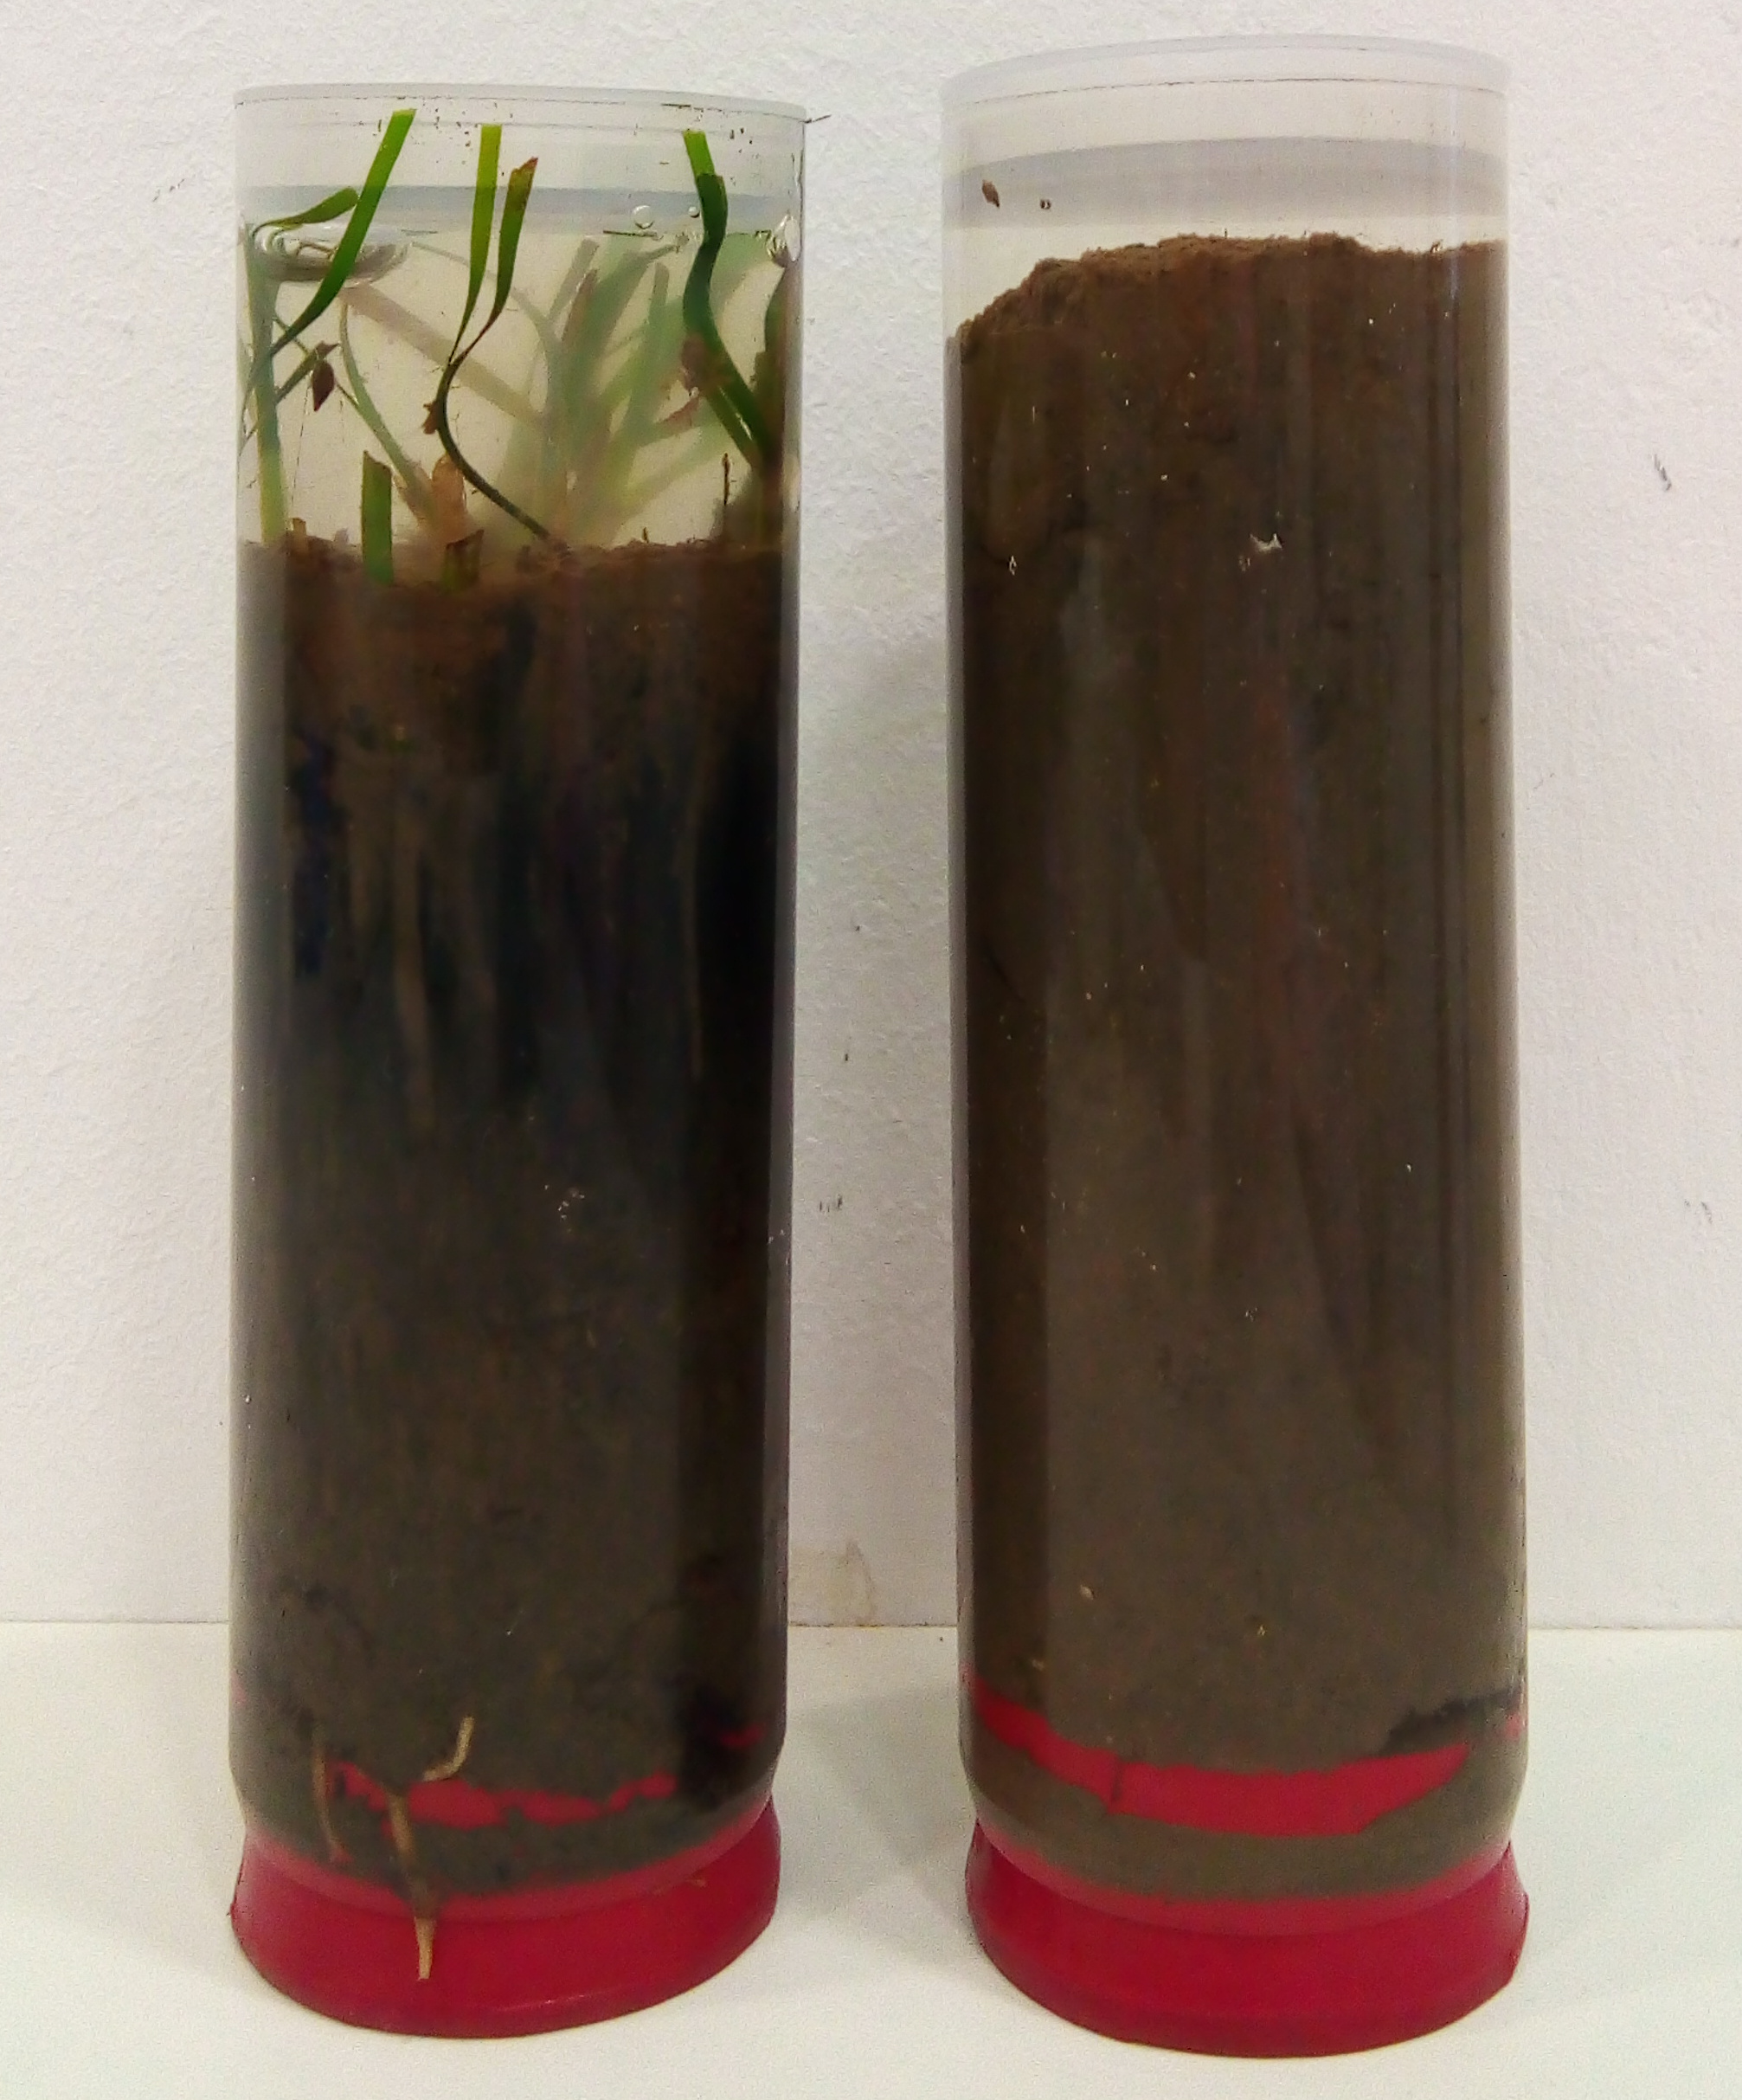
\includegraphics[width=0.55\linewidth]{figures/sediment-cores-2017-09-14} 

}

\caption{Sediment cores sampled on 14 September 2017 in the Bay of Saline in the \emph{Cymodocea nodosa} seagrass meadow (vegetated site; left) and in the adjacent area without seagrass vegetation (nonvegetated site; right). The black zone, which is indicative of the formation of iron sulphides, is visible in the sediment core sampled from the vegetated site (left). The length of the plastic core sampler is 15 \si{\cm}.}\label{fig:sediment-cores-2017-09-14}
\end{figure}



The taxonomic classification of the obtained partial 16S rRNA sequences showed the dominance of the domain \emph{Bacteria} over the domain \emph{Archaea}. The bacterial community consisted mainly of \emph{Desulfobacterota}, \emph{Gammaproteobacteria}, \emph{Bacteroidota}, \emph{Chloroflexi}, \emph{Planctomycetota}, and \emph{Campylobacterota}, while the archaeal community mainly comprised \emph{Nanoarchaeota}, \emph{Thermoplasmatota}, \emph{Crenarchaeota}, and \emph{Asgardarchaeota}. All of these taxa are typical of marine sediments (\protect\hyperlink{ref-Hoshino2020}{Hoshino et al., 2020}; \protect\hyperlink{ref-Sun2020}{Sun et al., 2020}; \protect\hyperlink{ref-Walsh2016a}{Walsh et al., 2016}; \protect\hyperlink{ref-Zheng2019}{Zheng et al., 2019}), with \emph{Campylobacterota} being characteristic of the seagrass rhizosphere (\protect\hyperlink{ref-Ettinger2017}{Ettinger et al., 2017}; \protect\hyperlink{ref-Jensen2007}{Jensen et al., 2007}). The observed trend of the proportion of archaea increasing with sediment depth and the proportion of bacteria decreasing is similar to trends observed for deeper sediment cores, which show a dominance of bacteria in the upper sediment parts and a similar proportion of bacteria and archaea in the deeper sediment (\protect\hyperlink{ref-Chen2017}{Chen et al., 2017}). In addition to this general trend, the main taxa whose proportion changed with sediment depth were \emph{Thermoplasmatota}, \emph{Chloroflexi}, \emph{Gammaproteobacteria}, and \emph{Bacteroidota}. The increase in the proportion of \emph{Thermoplasmatota} and \emph{Chloroflexi} with sediment depth and the simultaneous decrease in the proportion of \emph{Gammaproteobacteria} could be related to the measured general oxygen depletion after the first centimetre of sediment. Studies have associated Marine Benthic Group D and DHVEG-1, which make up the majority of \emph{Thermoplasmatota} sequences in the sediment of the Bay of Saline, and \emph{Chloroflexi} with anoxic sediments, while \emph{Gammaproteobacteria} are more characteristic of oxic sediments (\protect\hyperlink{ref-Durbin2011}{Durbin and Teske, 2011}; \protect\hyperlink{ref-Hoshino2020}{Hoshino et al., 2020}; \protect\hyperlink{ref-Lloyd2013}{Lloyd et al., 2013}). In addition to oxygen depletion, the availability of fresh organic matter could also influence the changes in the proportion of microbial taxa with sediment depth. The ability of \emph{Gammaproteobacteria} and \emph{Bacteroidota} to degrade and assimilate fresh detritus in coastal sediments may have influenced the decline in their relative abundance with sediment depth, as it is known that fresh organic matter content is less available in deeper sediment layers (\protect\hyperlink{ref-Gihring2009}{Gihring et al., 2009}; \protect\hyperlink{ref-Middelburg1989}{Middelburg, 1989}).

In contrast to the analysis of the V4 region of the 16S rRNA gene, which showed that the microbial communities in the sediment were primarily stratified by sediment depth and secondarily differed between the vegetated and nonvegetated site, the main factor influencing the microbial metabolic profile was the decline of the \emph{C. nodosa} seagrass meadow. The influence of decline was observed in protein richness and diversity, the structure of the metabolic profile, and the assessed proteins involved in organic matter degradation. The influences of sediment depth or site were secondary; that is, the effects of seagrass meadow decline were not observed or were not of the same magnitude at each site and in every layer. Due to the primary influence of seagrass decline, the effect of sediment depth on the microbial metabolic profile is discussed in detail below in Section \ref{section-temporal-differences}, where the effects of seagrass decline are considered.

\hypertarget{section-site-differences}{%
\section{Site differences: influence of seagrass cover}\label{section-site-differences}}

Sampling sediment cores from two sites, one with a declining \emph{Cymodocea nodosa} meadow (vegetated site) and the other without seagrass vegetation (nonvegetated site), made it possible to assess the influence of seagrass cover on the microbes in the sediment. As previously mentioned, the analysis of the V4 region of the 16S rRNA gene revealed that the microbial communities in the sediment showed differences between the vegetated and nonvegetated site. These differences were also suggested on some sampling dates by the distinct visual appearance of the sediment cores from the vegetated and nonvegetated site as shown in Figure \ref{fig:sediment-cores-2017-09-14}. Changes in alpha diversity with sediment depth were only observed in the vegetated sediment. As these differences between sites are related to sediment depth, they are discussed in detail in Section \ref{section-sediment-depth} when the changes with sediment depth are considered. The observed differences in microbial communities between sites are not surprising, as it is known that communities in marine sediments are site-specific (\protect\hyperlink{ref-Hamdan2013}{Hamdan et al., 2013}; \protect\hyperlink{ref-Polymenakou2005}{Polymenakou et al., 2005}), which may only be more pronounced if one of the sites is influenced by seagrass cover. Indeed, data have shown that microbial communities in the sediment differ not only between areas with and without vegetation (\protect\hyperlink{ref-Alsaffar2020}{Alsaffar et al., 2020}; \protect\hyperlink{ref-Smith2004}{A. Smith et al., 2004}; \protect\hyperlink{ref-Sun2020}{Sun et al., 2020}; \protect\hyperlink{ref-Zheng2019}{Zheng et al., 2019}), but also between the periphery and the central region of the seagrass meadow (\protect\hyperlink{ref-Ettinger2017}{Ettinger et al., 2017}). Although the communities from the vegetated and nonvegetated sediment showed differences, there was still a high degree of overlap in community composition. The highest degree of overlap was observed in the top sediment layer. These observations are not surprising as the microbes living in these sediments likely originate from the same source and only undergo site-specific selection through burial (\protect\hyperlink{ref-Hamdan2013}{Hamdan et al., 2013}; \protect\hyperlink{ref-Petro2019}{Petro et al., 2019}; \protect\hyperlink{ref-Walsh2016a}{Walsh et al., 2016}). In addition, the observed highest degree of overlap in community composition in the top sediment layer could be due not only to the same source of origin of the microbes, but also to the same carbon source, as seagrass detritus is one of the main carbon sources in \emph{C. nodosa} meadows and can be imported into the nonvegetated site (\protect\hyperlink{ref-Holmer2004}{Holmer et al., 2004}).

Taxonomic analysis of the partial 16S rRNA sequences obtained revealed differences between the vegetated and nonvegetated sites for some groups. \emph{Crenarchaeota} and \emph{Gammaproteobacteria} showed a higher proportion in the sediment of the nonvegetated site, while the proportion of \emph{Bacteroidota} and \emph{Campylobacterota} was higher in the vegetated sediment. Interestingly, different groups within the \emph{Desulfobacterota} showed different affinities, with \emph{Desulfosarcinaceae} showing a higher proportion in the vegetated sediment and \emph{Desulfobulbaceae} in the nonvegetated sediment. The differences in proportions observed for \emph{Crenarchaeota} between sites were the result of the much greater increase in \emph{Bathyarcheia}, the major component of \emph{Crenarchaeota} in the Bay of Saline, with increasing sediment depth at the nonvegetated site. \emph{Bathyarcheia}, formerly known as the Miscellaneous Crenarchaeotal Group (MCG), are well adapted to energy limitation and are usually found in deeper sediment layers (\protect\hyperlink{ref-Kubo2012}{Kubo et al., 2012}). It is possible that the presence of \emph{C. nodosa} has caused the observed lower proportion of this group in the vegetated sediment, as seagrasses enrich the sediment with organic matter directly or through various seagrass-mediated processes (\protect\hyperlink{ref-Duarte2005}{Duarte, Holmer, et al., 2005}; \protect\hyperlink{ref-Liu2017}{Liu et al., 2017}; \protect\hyperlink{ref-Peduzzi1991}{Peduzzi and Herndl, 1991}; \protect\hyperlink{ref-Terrados2000}{Terrados and Duarte, 2000}; \protect\hyperlink{ref-Trevathan-Tackett2020}{Trevathan-Tackett et al., 2020}; \protect\hyperlink{ref-vanKatwijk2010}{van Katwijk et al., 2010}). The higher proportion of \emph{Gammaproteobacteria} in the nonvegetated sediment could, like its higher proportion in the top sediment layer (\protect\hyperlink{ref-Durbin2011}{Durbin and Teske, 2011}; \protect\hyperlink{ref-Hoshino2020}{Hoshino et al., 2020}), be related to oxygen availability, as oxygen penetration depth was generally higher in the nonvegetated sediment. Indeed, Ettinger et al. (\protect\hyperlink{ref-Ettinger2017}{2017}) also found a higher proportion of \emph{Gammaproteobacteria} in the sediment outside the seagrass meadow than inside it. \emph{Thioalkalispiraceae}, one of the main groups within the \emph{Gammaproteobacteria}, showed a strong difference in proportion between sites. The higher proportion of this group in the nonvegetated sediment could be related to the lower organic matter content in this sediment, as \emph{Thioalkalispiraceae} are known to be chemolithoautotrophic (\protect\hyperlink{ref-Mori2011}{Mori et al., 2011}; \protect\hyperlink{ref-Mori2014}{Mori and Suzuki, 2014}) and may rely on inorganic compounds rather than the organic matter provided by the seagrass.

In contrast to the proportion of \emph{Crenarchaeota} and \emph{Gammaproteobacteria}, the proportion of \emph{Bacteroidota} and \emph{Campylobacterota} was higher in the vegetated sediment. The higher proportion of \emph{Bacteroidota} in the sediment of the vegetated site could be related to the higher content of plant material in this sediment. Members of \emph{Bacteroidota} have been identified as decomposers of macromolecules such as cellulose (\protect\hyperlink{ref-Thomas2011}{Thomas et al., 2011}), and similar to angiosperm land plants, cellulose is the main component of seagrass cell walls (\protect\hyperlink{ref-Pfeifer2020}{Pfeifer and Classen, 2020}; \protect\hyperlink{ref-Syed2016}{Syed et al., 2016}; \protect\hyperlink{ref-Torbatinejad2001}{Torbatinejad and Sabin, 2001}). The higher proportion of \emph{Campylobacterota} in the vegetated sediment is not surprising, as this group and especially members of its family \emph{Sulfurimonadaceae} are known to be closely associated with seagrass roots and rhizomes (\protect\hyperlink{ref-Ettinger2017}{Ettinger et al., 2017}; \protect\hyperlink{ref-Jensen2007}{Jensen et al., 2007}). In the Bay of Saline, the \emph{Sulfurimonadaceae} also accounted for a high proportion of the sequences classified as \emph{Campylobacterota} in the vegetated sediment. The proximity of the sampled sediment to seagrass roots and rhizomes probably influenced the higher proportion of \emph{Campylobacterota} and consequently of \emph{Sulfurimonadaceae} in the vegetated sediment. Since seagrasses are known to select the microbial community in the rhizosphere from the bulk sediment by enriching some taxa and depleting others (\protect\hyperlink{ref-Cucio2016}{Cúcio et al., 2016}; \protect\hyperlink{ref-Zhang2020}{X. Zhang et al., 2020}, \protect\hyperlink{ref-Zhang2022}{2022}), it is possible that seagrass roots and rhizomes alter the microbial community composition in the nearby sediment to some extent in a similar manner.

In general, \emph{Desulfobacterota} was the most abundant high-taxonomic rank in the sediment microbial community in the Bay of Saline. This is consistent with other studies that have identified \emph{Desulfobacterota} as one of the major high-taxonomic ranks in the sediment colonised by seagrass (\protect\hyperlink{ref-Cucio2016}{Cúcio et al., 2016}; \protect\hyperlink{ref-Ettinger2017}{Ettinger et al., 2017}; \protect\hyperlink{ref-Garcia-Martinez2009}{García-Martínez et al., 2009}). Although the proportion of \emph{Desulfobacterota} did not show strong differences between sites or with increasing sediment depth, some groups within this phylum showed a different affinity for vegetated and nonvegetated sediment, as previously mentioned. The observed higher proportion of \emph{Desulfosarcinaceae} in the vegetated sediment and \emph{Desulfobulbaceae} in the nonvegetated sediment is consistent with previous studies that reported a high proportion of \emph{Desulfosarcina}-related sequences in seagrass-vegetated sediments and a higher number of sequences related to \emph{Desulfobulbaceae} in the nonvegetated sediment (\protect\hyperlink{ref-Garcia-Martinez2009}{García-Martínez et al., 2009}; \protect\hyperlink{ref-Smith2004}{A. Smith et al., 2004}). In addition, the high metabolic versatility of \emph{Desulfosarcinaceae} (\protect\hyperlink{ref-Watanabe2020}{Watanabe et al., 2020}) may have led to their greater proliferation in vegetated sediment, where high concentrations of various carbon substrates may become available during organic matter decomposition (\protect\hyperlink{ref-Duarte2005}{Duarte, Holmer, et al., 2005}; \protect\hyperlink{ref-Liu2017}{Liu et al., 2017}; \protect\hyperlink{ref-Peduzzi1991}{Peduzzi and Herndl, 1991}; \protect\hyperlink{ref-Trevathan-Tackett2020}{Trevathan-Tackett et al., 2020}).

As already mentioned (Section \ref{section-sediment-depth}), the main factor influencing the metabolic profile of the microbial communities in the sediment was the decline of the \emph{C. nodosa} meadow, while the influence of sediment depth and site were secondary. The influence of site and thus of seagrass cover was particularly evident before the decline of seagrass, especially in the deeper sediment layers. This effect was observed in protein richness and diversity, the structure of the metabolic profile, and the assessed proteins involved in organic matter degradation. Due to the primary influence of seagrass decline, the effect of the sampling site on the metabolic profile of the microbial communities in the sediment is discussed in detail in Section \ref{section-temporal-differences}, where the effects of seagrass decline are considered.

\hypertarget{section-temporal-differences}{%
\section{Temporal differences: influence of seagrass decline}\label{section-temporal-differences}}

The analysis of a comprehensive set of 118 metaproteomes, whose proteins were identified by searching a database composed of the sequenced metagenomes, made it possible to assess the dynamics of the metabolic profile of the microbial sediment communities in the Bay of Saline. In addition, the sampling of sediment cores in the period before and during the decline of a \emph{Cymodocea nodosa} meadow allowed the assessment of the temporal dynamics and thus the influence of seagrass decline on the same metabolic profile. The influence of the decline of the meadow was observed in protein richness and diversity, the structure of the metabolic profile, and the assessed proteins involved in organic matter degradation. Prior to the decline, higher values of the number of observed proteins and the exponential of the Shannon diversity index were found in the vegetated sediment compared to the nonvegetated sediment. Moreover, these differences were more pronounced in the deeper parts of the sediments, i.e.~in the lower middle and bottom layer (Figure \ref{fig:influence-seagrass-decline}). The differences between the sites began to disappear during the decline of the meadow and the values of the number of observed proteins and the exponential of the Shannon diversity index were similar to those found in the sediment previously inhabited by the meadow. In addition to these differences, the structure of the metabolic profile of the sediment communities of the nonvegetated site also showed temporal differences. A separation was found between the period before and during the decline of the meadow, especially in the deeper parts of the sediment and when only proteins belonging to the Cluster of Orthologous Genes (COG) category C, which includes proteins for energy production and conversion, were considered. In contrast, no temporal pattern was found for the communities of the vegetated site (Figure \ref{fig:influence-seagrass-decline}).
\newpage

\begin{figure}[ht!]

{\centering 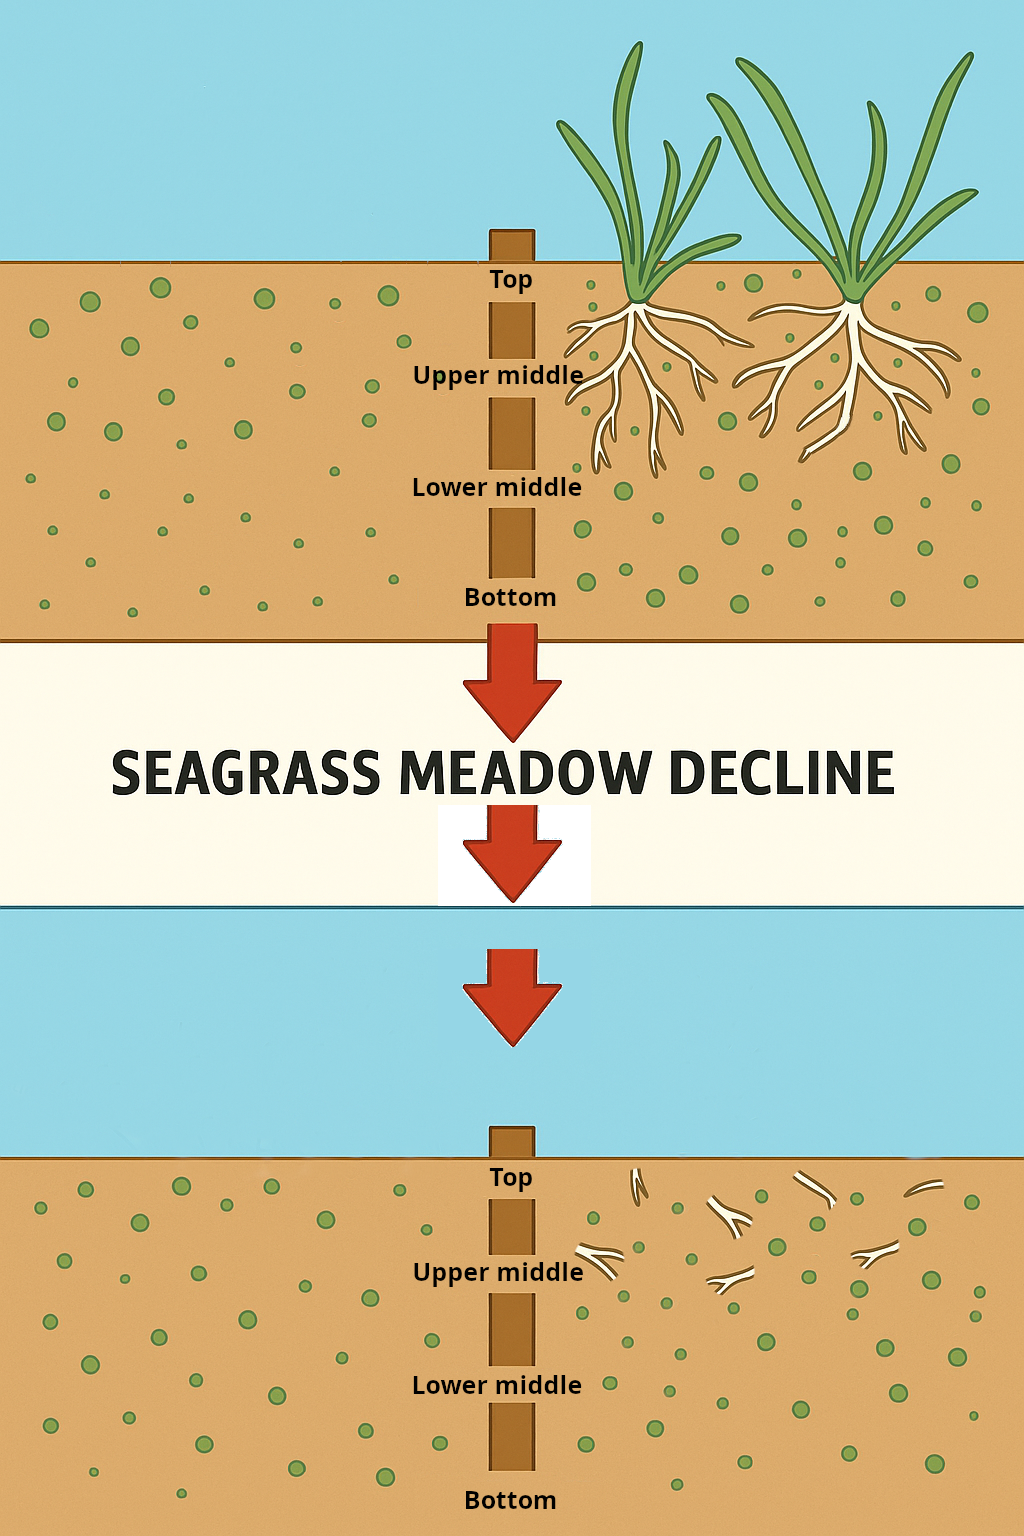
\includegraphics[width=0.65\linewidth]{figures/influence-seagrass-decline} 

}

\caption{A conceptual diagram illustrating the shift in the metabolic profile (green dots) of sediment microbial communities during the decline of a \emph{Cymodocea nodosa} meadow in the Bay of Saline. Prior to the decline (upper panel), differences in metabolic profiles were observed between the vegetated and nonvegetated site, particularly in the deeper sediment layers. During the decline (lower panel), these differences diminished and the metabolic profile of the nonvegetated site began to resemble that of the vegetated site. The analysis was based on sediment cores cut into four sections of 1 \si{\cm} length each: the top (0--1 \si{\cm}), the bottom (7--8 \si{\cm}), and two middle sections: upper middle (2--3 \si{\cm}) and lower middle (3--6 \si{\cm}).}\label{fig:influence-seagrass-decline}
\end{figure}



Differences between sites discussed in Section \ref{section-site-differences} were accompanied by differences in metabolic profiles between sites observed prior to decline of the meadow. This is not surprising, as data have shown that microbial communities in vegetated sediments differ in composition (\protect\hyperlink{ref-Alsaffar2020}{Alsaffar et al., 2020}; \protect\hyperlink{ref-Ettinger2017}{Ettinger et al., 2017}; \protect\hyperlink{ref-Sun2020}{Sun et al., 2020}; \protect\hyperlink{ref-Zheng2019}{Zheng et al., 2019}) and function (\protect\hyperlink{ref-Mohapatra2022}{Mohapatra et al., 2022}) from communities in nonvegetated sediments. The higher protein richness and diversity observed at the vegetated site prior to meadow decline is consistent with other studies reporting higher metabolic diversity and microbial activity in sediments colonised by seagrasses, which may be related to the higher organic matter content in these sediments (\protect\hyperlink{ref-Duarte2005}{Duarte, Holmer, et al., 2005}; \protect\hyperlink{ref-Holmer1997}{Holmer and Nielsen, 1997}; \protect\hyperlink{ref-Mohapatra2022}{Mohapatra et al., 2022}; \protect\hyperlink{ref-Smith2004}{A. Smith et al., 2004}). Furthermore, the greater differentiation in protein richness and diversity between sites over the same time period in the deeper parts of the sediment is consistent with the previously discussed results showing greater separation in community composition between sites in these parts of the sediment. In contrast, the lack of such differentiation of the same parameters in the upper parts of the sediment, i.e.~in the top and upper middle layer, could be explained by the input of seagrass-derived organic matter into the nonvegetated site, as organic matter from the \emph{C. nodosa} meadow can be imported into the nonvegetated site and has been shown to be an important source for the prokaryotes living in this sediment (\protect\hyperlink{ref-Holmer2004}{Holmer et al., 2004}). These observations are also supported by the dynamics of the structure of the metabolic profile observed at the nonvegetated site, which showed that samples originating from the upper parts of the sediment were grouped together regardless of the period of sampling.

The lack of differences in protein richness and diversity between sites during the decline of the meadow suggests a more uniform metabolic profile of the microbial communities in the sediment during this period, similar to the metabolic profile of the communities of the vegetated site prior to the decline. Furthermore, this observation is supported by the dynamics of the structure of the metabolic profile observed at the nonvegetated site. Samples collected during the decline grouped with samples collected in the upper parts of the sediment before the decline. As seagrass meadows are known to stabilise the sediment by reducing its resuspension and mixing (\protect\hyperlink{ref-Duarte2005}{Duarte, Holmer, et al., 2005}; \protect\hyperlink{ref-Terrados2000}{Terrados and Duarte, 2000}; \protect\hyperlink{ref-vanKatwijk2010}{van Katwijk et al., 2010}), the lack of differentiation between sites during the decline of the meadow could be the result of a greater input of fresh organic matter into the nonvegetated sediment due to increased resuspension, mixing, and transport between sites when the meadow is no longer present. Indeed, during the decline of the meadow from May to August 2018, higher concentrations of total lipids and organic matter were detected at the nonvegetated than at the vegetated site. In contrast, the uniformity of the microbial profile observed at the vegetated site throughout the study period could be the result of maintaining the source of organic matter during the decline due to decay of leaves, roots, and rhizomes (\protect\hyperlink{ref-Duarte2005}{Duarte, Holmer, et al., 2005}; \protect\hyperlink{ref-Liu2017}{Liu et al., 2017}; \protect\hyperlink{ref-Peduzzi1991}{Peduzzi and Herndl, 1991}; \protect\hyperlink{ref-Trevathan-Tackett2020}{Trevathan-Tackett et al., 2020}).

Given the great importance of sediments colonised by seagrasses for carbon sequestration and the role of microbial communities in these habitats in the mineralisation of organic matter (\protect\hyperlink{ref-Duarte2005a}{Duarte, Middelburg, et al., 2005}; \protect\hyperlink{ref-Duarte2013}{Duarte et al., 2013}; \protect\hyperlink{ref-Kennedy2010}{Kennedy et al., 2010}), it is interesting to evaluate the dynamics of microbial proteins involved in the degradation of organic matter during such an ecological event as the decline of a seagrass meadow. In addition, analysis of the functional COG categories showed that category C, which includes proteins for energy production and conversion, is the most abundant. This is consistent with metagenomic studies, which also found that energy production and conversion is one of the most abundant functional COG categories in coastal sediments (\protect\hyperlink{ref-Habibi2023}{Habibi et al., 2023}). Proteins involved in organic matter degradation were assessed by analysing the dynamics of hydrolytic enzymes, ATP-binding cassette (ABC) transporters, fermentation-mediating enzymes, and proteins involved in dissimilatory sulphate reduction. The analysis of hydrolytic enzymes showed that Carbohydrate-Active enZymes (CAZymes) and peptidases were more abundant than lipases, indicating the importance of carbohydrates and proteins as sources of organic matter for the microbes in the sediment of the Bay of Saline. Among the CAZymes, the glycoside hydrolase families GH5 and GH9, which contain members that can hydrolyse plant organic matter such as cellulose, were the most abundant (\protect\hyperlink{ref-Aspeborg2012}{Aspeborg et al., 2012}; \protect\hyperlink{ref-Berlemont2016}{Berlemont and Martiny, 2016}; \protect\hyperlink{ref-Drula2022}{Drula et al., 2022}). This is not surprising since, as already mentioned, cellulose is the main component of the cell walls of seagrasses (\protect\hyperlink{ref-Pfeifer2020}{Pfeifer and Classen, 2020}; \protect\hyperlink{ref-Syed2016}{Syed et al., 2016}; \protect\hyperlink{ref-Torbatinejad2001}{Torbatinejad and Sabin, 2001}). The peptidases consisted almost exclusively of metalloendopeptidases and serine endopeptidases, similar to other coastal sediments where high proportions of these enzymes were found among the extracellular proteases (\protect\hyperlink{ref-Liu2023}{Z. Liu et al., 2023}; \protect\hyperlink{ref-Zhang2015a}{X.-Y. Zhang et al., 2015}; \protect\hyperlink{ref-Zhou2013}{M.-Y. Zhou et al., 2013}). In general, CAZymes and peptidases showed no response to meadow decline, except that the proportion of CAZymes in the top sediment layer of the nonvegetated site decreased from pre-decline to meadow decline, while the proportion of peptidases in the upper middle sediment layer of the vegetated site increased during the same period. These patterns could be explained by the increased microbial colonisation of detritus and microbial utilisation of exogenous nitrogen during seagrass tissue decomposition, as studies have shown that the molar carbon:nitrogen content in seagrass litter decreases during this process (\protect\hyperlink{ref-Liu2017}{Liu et al., 2017}; \protect\hyperlink{ref-Peduzzi1991}{Peduzzi and Herndl, 1991}).

Prokaryotes utilise various transport proteins, including ABC transporters (\protect\hyperlink{ref-Davidson2004}{Davidson and Chen, 2004}), to import hydrolytic products into the cell. The proportion of ABC transporters found in the sediment of the Bay of Saline is consistent with other studies that have also found a high abundance of these transporters in marine sediments (\protect\hyperlink{ref-Habibi2023}{Habibi et al., 2023}; \protect\hyperlink{ref-Wang2020a}{S. Wang et al., 2020}). Among the ABC transporters, those for sugars and amino acids were the most abundant and their dynamics reflected the overall dynamics of the metabolic profile. Before the decline of the meadow, ABC transporters for sugars showed a higher proportion in the deeper parts of the vegetated sediment than in the nonvegetated sediment. This distribution pattern reflects the higher organic matter content and thus the greater demand for ABC transporters in vegetated sediments (\protect\hyperlink{ref-Duarte2005}{Duarte, Holmer, et al., 2005}; \protect\hyperlink{ref-Mohapatra2022}{Mohapatra et al., 2022}). In contrast, these ABC transporters did not show different proportions between sites during the decline of the meadow. In addition, the ABC transporters for sugars and amino acids showed an increase in their proportion in the bottom sediment layer at the nonvegetated site from before the decline to the decline of the meadow, which could be the result of a greater input of fresh organic matter into the nonvegetated sediment during the decline (\protect\hyperlink{ref-Duarte2005}{Duarte, Holmer, et al., 2005}; \protect\hyperlink{ref-Terrados2000}{Terrados and Duarte, 2000}; \protect\hyperlink{ref-vanKatwijk2010}{van Katwijk et al., 2010}), as previously mentioned.

The organic matter in anoxic sediments is mineralised in an anaerobic food chain in which fermentation processes carried out by microbes are an essential component (\protect\hyperlink{ref-Arndt2013}{Arndt et al., 2013}). Among the fermentation-mediating enzymes analysed, formate dehydrogenase, pyruvate:ferredoxin oxidoreductase, and alcohol dehydrogenase were the most abundant. This is not surprising, as microcosm studies of the anaerobic degradation of organic matter in marine sediments have found acetate, formate, and ethanol to be the most common fermentation products (\protect\hyperlink{ref-Graue2012}{Graue et al., 2012}; \protect\hyperlink{ref-Pelikan2021}{Pelikan et al., 2021}), while direct measurements of sediment pore water have demonstrated the presence of methanol and ethanol (\protect\hyperlink{ref-Zhuang2014}{Zhuang et al., 2014}). In addition, pyruvate:ferredoxin oxidoreductase and alcohol dehydrogenase have been reported to be important fermentation-mediating enzymes in Baltic Sea sediments (\protect\hyperlink{ref-Zinke2019}{Zinke et al., 2019}). Similar to the dynamics of the ABC transporters, the dynamics of the fermentation-mediating enzymes also reflected the overall changes of the metabolic profile. Prior to the decline of the meadow, the proportion of formate dehydrogenase, pyruvate:ferredoxin oxidoreductase, and alcohol dehydrogenase was found to be higher in the deeper parts of the sediment at the vegetated site than at the nonvegetated site, reflecting the higher organic matter content and possibly a higher fermentation rate in the seagrass-colonised sediments (\protect\hyperlink{ref-Duarte2005}{Duarte, Holmer, et al., 2005}; \protect\hyperlink{ref-Mohapatra2022}{Mohapatra et al., 2022}).

Given that dissimilatory sulphate reduction is recognised as the predominant terminal pathway of organic matter mineralisation in anoxic seabeds (\protect\hyperlink{ref-Jorgensen1982}{Jørgensen, 1982}; \protect\hyperlink{ref-Jorgensen2019}{Jørgensen et al., 2019}), that \emph{Desulfobacterota}, a group known to contain sulphate reducers found in marine sediments, was the most abundant high-taxonomic rank in the sediment microbial community in the Bay of Saline, and that one of the most abundant proteins in the functional COG category C was adenylylsulphate reductase, a protein known to be involved in dissimilatory sulphate reduction, it is interesting to assess the dynamics of the enzymes involved in this process in more detail. The metaproteomes of the microbial community in the sediment of the Bay of Saline contained sulphate adenylyltransferase (Sat), adenylylsulphate reductase (Apr), and dissimilatory sulphite reductase (Dsr), enzymes involved in the dissimilatory sulphate reduction pathway and shared by known sulphate-reducing microbes (\protect\hyperlink{ref-Jorgensen2019}{Jørgensen et al., 2019}). These enzymes showed changes comparable to the dynamics of the overall metabolic profile. In general, the proportion of these enzymes was higher in the deeper parts of the sediment at the vegetated site than at the nonvegetated site before the decline of the meadow, while such differences were not observed during the decline. Similar to the dynamics of the overall metabolic profile, these observations could be explained by the higher organic matter content in the seagrass-colonised sediments before the decline (\protect\hyperlink{ref-Duarte2005}{Duarte, Holmer, et al., 2005}; \protect\hyperlink{ref-Mohapatra2022}{Mohapatra et al., 2022}) and by a greater input of fresh organic matter into the nonvegetated sediment during the decline (\protect\hyperlink{ref-Duarte2005}{Duarte, Holmer, et al., 2005}; \protect\hyperlink{ref-Terrados2000}{Terrados and Duarte, 2000}; \protect\hyperlink{ref-vanKatwijk2010}{van Katwijk et al., 2010}), as previously mentioned.

In contrast to all these observations of the dynamics of the microbial metabolic profile, the community composition determined by analysing the V4 region of the 16S rRNA gene showed no temporal dynamics and thus no influence of the decline of the seagrass meadow. Even when the composition was analysed in a way that excludes the previously established influence of sediment depth and sampling site, no grouping of communities by month, year, or the period before and during seagrass meadow decline could be observed. Such a stable community composition and, in contrast, a dynamic metabolic profile could be the result of a large amount of extracellular DNA or a large proportion of dormant or dead microbial cells in marine sediments (\protect\hyperlink{ref-Bradley2019}{Bradley et al., 2019}; \protect\hyperlink{ref-Cangelosi2014}{Cangelosi and Meschke, 2014}; \protect\hyperlink{ref-Carini2016}{Carini et al., 2016}; \protect\hyperlink{ref-Jones2010}{S. E. Jones and Lennon, 2010}; \protect\hyperlink{ref-Luna2002}{Luna et al., 2002}; \protect\hyperlink{ref-Torti2015}{Torti et al., 2015}, \protect\hyperlink{ref-Torti2018}{2018}). It is estimated that over 80\si{\percent} of DNA in marine sediments is extracellular (\protect\hyperlink{ref-DellAnno2002}{Dell'Anno et al., 2002}; \protect\hyperlink{ref-DellAnno2005}{Dell'Anno and Danovaro, 2005}). Furthermore, dead cells can account for up to 70\si{\percent} of all bacterial cells in coastal marine sediments, while only 4\si{\percent} of living cells are actively growing (\protect\hyperlink{ref-Luna2002}{Luna et al., 2002}). Molecular techniques such as 16S rRNA gene sequencing or metagenomics are usually based on the isolation of total DNA and therefore cannot distinguish whether the DNA originates from living, dead, active, or dormant cells or the extracellular DNA pool (\protect\hyperlink{ref-Cangelosi2014}{Cangelosi and Meschke, 2014}; \protect\hyperlink{ref-Torti2015}{Torti et al., 2015}). In addition, the metabolic versatility of the microbes may contribute to some extent to the observed community stability, as the same community members may start to perform different metabolic functions during the decline of the seagrass meadow (\protect\hyperlink{ref-Bowen2011}{Bowen et al., 2011}; \protect\hyperlink{ref-Louca2018}{Louca et al., 2018}). Also, a longer sampling period after the loss of the seagrass meadow may be required to observe the changes in community composition, as the microbes living in marine sediments often have very long generation times (\protect\hyperlink{ref-Jorgensen2016}{Jørgensen and Marshall, 2016}; \protect\hyperlink{ref-Starnawski2017}{Starnawski et al., 2017}). The inability of the 16S rRNA gene sequencing approach to detect temporal changes in community composition highlights the importance of molecular techniques that enable functional characterisation, such as metaproteomics, in determining microbial response to environmental change in marine systems (\protect\hyperlink{ref-Saito2019}{Saito et al., 2019}).

\hypertarget{conclusions}{%
\chapter{CONCLUSIONS}\label{conclusions}}

Seagrass decline is a globally recognised issue with far-reaching consequences. While the effects of this decline on coastal ecosystems have been extensively documented, a critical aspect has been systematically overlooked, the sediment microbial community. Given the gap in previous research, this doctoral thesis addresses these knowledge gaps by providing a comprehensive analysis of sediment microbial communities throughout the decline of a seagrass meadow. Moreover, it offers the first detailed description of sediment microbial communities underlying a \emph{Cymodocea nodosa} seagrass meadow, for which only rhizosphere and epiphytic communities had previously been studied. In addition, it is among the first to use a combined metagenomic and metaproteomic approach to study microbial community metabolism, not only in seagrass sediments but also in coastal surface sediments, providing valuable data for further research.

This thesis consists of three scientific articles that represent a stepwise progression of research: the first (\textbf{Dynamics of environmental conditions during the decline of a \emph{Cymodocea nodosa} meadow}) documents the decline of the meadow alongside environmental conditions in the sediment; the second (\textbf{Compositional stability of sediment microbial communities during a seagrass meadow decline}) assesses the structure and dynamics of the sediment microbial communities; and the third (\textbf{Shift in the metabolic profile of sediment microbial communities during seagrass decline}) examines the metabolism of these microbial communities. The data presented in these scientific articles (Section 3) and discussed in Section 4 confirm the hypotheses:

\begin{enumerate}
\def\labelenumi{\arabic{enumi}.}
\tightlist
\item
  Decline of the \emph{C. nodosa} meadow alters sediment environmental conditions;
\end{enumerate}

It is clear that the decline of the seagrass meadow changed the environmental conditions in the sediment. In particular, an increase in hydrogen sulphide concentration and the expansion of its accumulation zone was observed during the decline of the meadow.

\begin{enumerate}
\def\labelenumi{\arabic{enumi}.}
\setcounter{enumi}{1}
\tightlist
\item
  The metabolic profile of the sediment microbial community differs with sediment depth, between the vegetated and nonvegetated sites, and throughout the study period;
\end{enumerate}

The metabolic profile of the sediment microbial communities was primarily influenced by the decline of the seagrass meadow. Before the seagrass decline, differences in the metabolic profile of the microbial communities in the sediment were observed between the seagrass-vegetated and the nonvegetated site, especially differing in the deeper sediment parts and not differing closer to the sediment surface. During the decline, these differences in the deeper sediment diminished and the metabolic profile of the microbial communities in the sediment at the nonvegetated site began to resemble that of the vegetated site.

Interestingly, the microbial community composition did not follow the same trend, allowing only for a partial confirmation of the hypothesis:

\begin{enumerate}
\def\labelenumi{\arabic{enumi}.}
\setcounter{enumi}{2}
\tightlist
\item
  The sediment microbial community structure differs with sediment depth, between the vegetated and nonvegetated sites, and throughout the study period;
\end{enumerate}

Analysis of the V4 region of the 16S rRNA gene clearly showed that the microbial communities in the sediment were primarily stratified by sediment depth and secondarily differed between the seagrass-vegetated and nonvegetated site. In contrast to the metabolic profile of the communities, no temporal changes and thus no response to the decline of the seagrass could be observed in the structure of the microbial communities.

\bigskip

Taken together the collected data once again confirm the previously established notion that vegetated sediments harbour distinct microbial communities from the ones found in the nonvegetated sediments, but also highlight the great influence of the seagrass meadow
on the adjacent nonvegetated sediment, reflected in a highly similar microbial community in upper sediment parts. Throughout meadow decline the microbial communities underlying the seagrass meadow exhibit great stability, while the communities of the deeper layers of the adjacent sediment remain compositionally the same and adapt their metabolic profile as a response to greater availability of fresh organic matter. These communities become highly similar to those found in the seagrass sediment throughout the whole sediment core, indicating the intensified spread of seagrass derived organic matter throughout the whole area, in turn fuelling organic matter decomposition accompanied by high concentrations of hydrogen sulphide. In conclusion, the clear influence of seagrass on a wide sediment area has been demonstrated through assessment of environmental parameters and the use of molecular methods. This influence was only more emphasised with meadow decline, highlighting the broader ecological influence of the decline of seagrass meadows. The comprehensive temporal dataset generated, including data of sediment environmental conditions, microbial community composition, and metabolic functions, provides a strong foundation for further studies on sediment microbial communities of seagrass meadows and coastal surface sediment in general.

\hypertarget{bibliography}{%
\chapter{BIBLIOGRAPHY}\label{bibliography}}

\hypertarget{refs}{}
\begin{CSLReferences}{1}{0}
\leavevmode\vadjust pre{\hypertarget{ref-Agostini2003}{}}%
Agostini, S., Pergent, G., and Marchand, B. (2003). Growth and primary production of {{\emph{Cymodocea nodosa}}} in a coastal lagoon. \emph{Aquatic Botany}, \emph{76}(3), 185--193. \url{https://doi.org/10.1016/S0304-3770(03)00049-4}

\leavevmode\vadjust pre{\hypertarget{ref-Alsaffar2020}{}}%
Alsaffar, Z., Pearman, J. K., Cúrdia, J., Ellis, J., Calleja, M. L., Ruiz-Compean, P., Roth, F., Villalobos, R., Jones, B. H., Morán, X. A. G., and Carvalho, S. (2020). The role of seagrass vegetation and local environmental conditions in shaping benthic bacterial and macroinvertebrate communities in a tropical coastal lagoon. \emph{Scientific Reports}, \emph{10}(1), 13550. \url{https://doi.org/10.1038/s41598-020-70318-1}

\leavevmode\vadjust pre{\hypertarget{ref-Amann1995}{}}%
Amann, R. I., Ludwig, W., and Schleifer, K. H. (1995). Phylogenetic identification and in situ detection of individual microbial cells without cultivation. \emph{Microbiological Reviews}, \emph{59}(1), 143--169. \url{https://doi.org/10.1128/mr.59.1.143-169.1995}

\leavevmode\vadjust pre{\hypertarget{ref-Apprill2015}{}}%
Apprill, A., McNally, S., Parsons, R., and Weber, L. (2015). Minor revision to {V4} region {SSU rRNA 806R} gene primer greatly increases detection of {SAR11} bacterioplankton. \emph{Aquatic Microbial Ecology}, \emph{75}(2), 129--137. \url{https://doi.org/10.3354/ame01753}

\leavevmode\vadjust pre{\hypertarget{ref-Arber1920}{}}%
Arber, A. (1920). \emph{Water plants: a study of aquatic angiosperms}. Cambridge University Press.

\leavevmode\vadjust pre{\hypertarget{ref-Arndt2013}{}}%
Arndt, S., Jørgensen, B. B., LaRowe, D. E., Middelburg, J. J., Pancost, R. D., and Regnier, P. (2013). Quantifying the degradation of organic matter in marine sediments: a review and synthesis. \emph{Earth-Science Reviews}, \emph{123}, 53--86. \url{https://doi.org/10.1016/j.earscirev.2013.02.008}

\leavevmode\vadjust pre{\hypertarget{ref-Arnosti2011}{}}%
Arnosti, C. (2011). Microbial extracellular enzymes and the marine carbon cycle. \emph{Annual Review of Marine Science}, \emph{3}, 401--425. \url{https://doi.org/10.1146/annurev-marine-120709-142731}

\leavevmode\vadjust pre{\hypertarget{ref-Aspeborg2012}{}}%
Aspeborg, H., Coutinho, P. M., Wang, Y., Brumer, H., and Henrissat, B. (2012). Evolution, substrate specificity and subfamily classification of glycoside hydrolase family 5 ({GH5}). \emph{BMC Evolutionary Biology}, \emph{12}(1), 186. \url{https://doi.org/10.1186/1471-2148-12-186}

\leavevmode\vadjust pre{\hypertarget{ref-Bargiela2015}{}}%
Bargiela, R., Herbst, F.-A., Martínez-Martínez, M., Seifert, J., Rojo, D., Cappello, S., Genovese, M., Crisafi, F., Denaro, R., Chernikova, T. N., Barbas, C., von Bergen, M., Yakimov, M. M., Ferrer, M., and Golyshin, P. N. (2015). Metaproteomics and metabolomics analyses of chronically petroleum-polluted sites reveal the importance of general anaerobic processes uncoupled with degradation. \emph{Proteomics}, \emph{15}(20), 3508--3520. \url{https://doi.org/10.1002/pmic.201400614}

\leavevmode\vadjust pre{\hypertarget{ref-Barsanti2007}{}}%
Barsanti, M., Delbono, I., Ferretti, O., Peirano, A., Bianchi, C. N., and Morri, C. (2007). Measuring change of {Mediterranean} coastal biodiversity: diachronic mapping of the meadow of the seagrass {{{\emph{Cymodocea nodosa}}} (Ucria) Ascherson in the Gulf of Tigullio (Ligurian Sea, NW Mediterranean)}. \emph{Hydrobiologia}, \emph{580}(1), 35--41. \url{https://doi.org/10.1007/s10750-006-0467-7}

\leavevmode\vadjust pre{\hypertarget{ref-Bent2008}{}}%
Bent, S. J., and Forney, L. J. (2008). The tragedy of the uncommon: understanding limitations in the analysis of microbial diversity. \emph{The ISME Journal}, \emph{2}(7), 689--695. \url{https://doi.org/10.1038/ismej.2008.44}

\leavevmode\vadjust pre{\hypertarget{ref-Berger1990}{}}%
Berger, W. H., and Wefer, G. (1990). Export production: seasonality and intermittency, and paleoceanographic implications. \emph{Global and Planetary Change}, \emph{3}(3), 245--254. \url{https://doi.org/10.1016/0031-0182(90)90065-F}

\leavevmode\vadjust pre{\hypertarget{ref-Berlemont2016}{}}%
Berlemont, R., and Martiny, A. C. (2016). Glycoside hydrolases across environmental microbial communities. \emph{PLOS Computational Biology}, \emph{12}(12), e1005300. \url{https://doi.org/10.1371/journal.pcbi.1005300}

\leavevmode\vadjust pre{\hypertarget{ref-Beulig2018}{}}%
Beulig, F., Røy, H., Glombitza, C., and Jørgensen, B. B. (2018). Control on rate and pathway of anaerobic organic carbon degradation in the seabed. \emph{Proceedings of the National Academy of Sciences of the United States of America}, \emph{115}(2), 367--372. \url{https://doi.org/10.1073/pnas.1715789115}

\leavevmode\vadjust pre{\hypertarget{ref-Bienhold2016}{}}%
Bienhold, C., Zinger, L., Boetius, A., and Ramette, A. (2016). Diversity and biogeography of bathyal and abyssal seafloor bacteria. \emph{PLOS One}, \emph{11}(1), e0148016. \url{https://doi.org/10.1371/journal.pone.0148016}

\leavevmode\vadjust pre{\hypertarget{ref-Blackburn1994}{}}%
Blackburn, T. H., Nedwell, D. B., and Wiebe, W. J. (1994). Active mineral cycling in a {Jamaican} seagrass sediment. \emph{Marine Ecology Progress Series}, \emph{110}(2--3), 233--239. \url{https://doi.org/10.3354/meps110233}

\leavevmode\vadjust pre{\hypertarget{ref-Borum2005}{}}%
Borum, J., Pedersen, O., Greve, T. M., Frankovich, T. A., Zieman, J. C., Fourqurean, J. W., and Madden, C. J. (2005). The potential role of plant oxygen and sulphide dynamics in die-off events of the tropical seagrass, {{\emph{Thalassia testudinum}}}. \emph{Journal of Ecology}, \emph{93}(1), 148--158. \url{https://doi.org/10.1111/j.1365-2745.2004.00943.x}

\leavevmode\vadjust pre{\hypertarget{ref-Boudouresque2009}{}}%
Boudouresque, C. F., Bernard, G., Pergent, G., Shili, A., and Verlaque, M. (2009). Regression of {Mediterranean} seagrasses caused by natural processes and anthropogenic disturbances and stress: a critical review. \emph{Botanica Marina}, \emph{52}(5), 395--418. \url{https://doi.org/10.1515/BOT.2009.057}

\leavevmode\vadjust pre{\hypertarget{ref-Boudreau1998}{}}%
Boudreau, B. P. (1998). Mean mixed depth of sediments: the wherefore and the why. \emph{Limnology and Oceanography}, \emph{43}(3), 524--526. \url{https://doi.org/10.4319/lo.1998.43.3.0524}

\leavevmode\vadjust pre{\hypertarget{ref-Bourque2015}{}}%
Bourque, A. S., Vega-Thurber, R., and Fourqurean, J. W. (2015). Microbial community structure and dynamics in restored subtropical seagrass sediments. \emph{Aquatic Microbial Ecology}, \emph{74}(1), 43--57. \url{https://doi.org/10.3354/ame01725}

\leavevmode\vadjust pre{\hypertarget{ref-Bowen2011}{}}%
Bowen, J. L., Ward, B. B., Morrison, H. G., Hobbie, J. E., Valiela, I., Deegan, L. A., and Sogin, M. L. (2011). Microbial community composition in sediments resists perturbation by nutrient enrichment. \emph{The ISME Journal}, \emph{5}(9), 1540--1548. \url{https://doi.org/10.1038/ismej.2011.22}

\leavevmode\vadjust pre{\hypertarget{ref-Bowles2014}{}}%
Bowles, M. W., Mogollón, J. M., Kasten, S., Zabel, M., and Hinrichs, K.-U. (2014). Global rates of marine sulfate reduction and implications for sub-sea-floor metabolic activities. \emph{Science}, \emph{344}(6186), 889--891. \url{https://doi.org/10.1126/science.1249213}

\leavevmode\vadjust pre{\hypertarget{ref-Bradley2019}{}}%
Bradley, J. A., Amend, J. P., and LaRowe, D. E. (2019). Survival of the fewest: microbial dormancy and maintenance in marine sediments through deep time. \emph{Geobiology}, \emph{17}(1), 43--59. \url{https://doi.org/10.1111/gbi.12313}

\leavevmode\vadjust pre{\hypertarget{ref-Brodersen2015}{}}%
Brodersen, K. E., Lichtenberg, M., Paz, L.-C., and Kühl, M. (2015). Epiphyte-cover on seagrass ({{\emph{Zostera marina}}} {L}.) leaves impedes plant performance and radial {O}{\textsubscript{2}} loss from the below-ground tissue. \emph{Frontiers in Marine Science}, \emph{2}, 58. \url{https://doi.org/10.3389/fmars.2015.00058}

\leavevmode\vadjust pre{\hypertarget{ref-Cancemi2002}{}}%
Cancemi, G., Buia, M. C., and Mazzella, L. (2002). Structure and growth dynamics of {{\emph{Cymodocea nodosa}}} meadows. \emph{Scientia Marina}, \emph{66}(4), 365--373. \url{https://doi.org/10.3989/scimar.2002.66n4365}

\leavevmode\vadjust pre{\hypertarget{ref-Canfield1993}{}}%
Canfield, D. E., Thamdrup, B., and Hansen, J. W. (1993). The anaerobic degradation of organic matter in {Danish} coastal sediments: iron reduction, manganese reduction, and sulfate reduction. \emph{Geochimica et Cosmochimica Acta}, \emph{57}(16), 3867--3883. \url{https://doi.org/10.1016/0016-7037(93)90340-3}

\leavevmode\vadjust pre{\hypertarget{ref-Cangelosi2014}{}}%
Cangelosi, G. A., and Meschke, J. S. (2014). Dead or alive: molecular assessment of microbial viability. \emph{Applied and Environmental Microbiology}, \emph{80}(19), 5884--5891. \url{https://doi.org/10.1128/AEM.01763-14}

\leavevmode\vadjust pre{\hypertarget{ref-Capo-Bauca2022}{}}%
Capó-Bauçà, S., Iñiguez, C., Aguiló-Nicolau, P., and Galmés, J. (2022). Correlative adaptation between {Rubisco} and {CO}{\textsubscript{2}}-concentrating mechanisms in seagrasses. \emph{Nature Plants}, \emph{8}(6), 706--716. \url{https://doi.org/10.1038/s41477-022-01171-5}

\leavevmode\vadjust pre{\hypertarget{ref-Carini2016}{}}%
Carini, P., Marsden, P. J., Leff, J. W., Morgan, E. E., Strickland, M. S., and Fierer, N. (2016). Relic {DNA} is abundant in soil and obscures estimates of soil microbial diversity. \emph{Nature Microbiology}, \emph{2}(3), 16242. \url{https://doi.org/10.1038/nmicrobiol.2016.242}

\leavevmode\vadjust pre{\hypertarget{ref-Carlson1994}{}}%
Carlson, Jr., Paul R., Yarbro, L. A., and Barber, T. R. (1994). Relationship of sediment sulfide to mortality of {{{\emph{Thalassia testudinum}}} in Florida Bay}. \emph{Bulletin of Marine Science}, \emph{54}(3), 733--746.

\leavevmode\vadjust pre{\hypertarget{ref-Cebrian1996}{}}%
Cebrián, J., Duarte, C. M., and Marbà, N. (1996). Herbivory on the seagrass {{{\emph{Cymodocea nodosa}}} (Ucria) Ascherson in contrasting Spanish Mediterranean habitats}. \emph{Journal of Experimental Marine Biology and Ecology}, \emph{204}(1), 103--111. \url{https://doi.org/10.1016/0022-0981(96)02574-9}

\leavevmode\vadjust pre{\hypertarget{ref-Cerqueira2018}{}}%
Cerqueira, T., Barroso, C., Froufe, H., Egas, C., and Bettencourt, R. (2018). Metagenomic signatures of microbial communities in deep-sea hydrothermal sediments of {Azores} vent fields. \emph{Microbial Ecology}, \emph{76}(2), 387--403. \url{https://doi.org/10.1007/s00248-018-1144-x}

\leavevmode\vadjust pre{\hypertarget{ref-Chefaoui2018}{}}%
Chefaoui, R. M., Duarte, C. M., and Serrão, E. A. (2018). Dramatic loss of seagrass habitat under projected climate change in the {Mediterranean Sea}. \emph{Global Change Biology}, \emph{24}(10), 4919--4928. \url{https://doi.org/10.1111/gcb.14401}

\leavevmode\vadjust pre{\hypertarget{ref-Chen2017}{}}%
Chen, X., Andersen, T. J., Morono, Y., Inagaki, F., Jørgensen, B. B., and Lever, M. A. (2017). Bioturbation as a key driver behind the dominance of bacteria over archaea in near-surface sediment. \emph{Scientific Reports}, \emph{7}(1), 2400. \url{https://doi.org/10.1038/s41598-017-02295-x}

\leavevmode\vadjust pre{\hypertarget{ref-Chourey2010}{}}%
Chourey, K., Jansson, J., VerBerkmoes, N., Shah, M., Chavarria, K. L., Tom, L. M., Brodie, E. L., and Hettich, R. L. (2010). Direct cellular lysis/protein extraction protocol for soil metaproteomics. \emph{Journal of Proteome Research}, \emph{9}(12), 6615--6622. \url{https://doi.org/10.1021/pr100787q}

\leavevmode\vadjust pre{\hypertarget{ref-Costa2015}{}}%
Costa, M. M., Barrote, I., Silva, J., Olivé, I., Alexandre, A., Albano, S., and Santos, R. (2015). Epiphytes modulate {{\emph{Posidonia oceanica}}} photosynthetic production, energetic balance, antioxidant mechanisms, and oxidative damage. \emph{Frontiers in Marine Science}, \emph{2}, 111. \url{https://doi.org/10.3389/fmars.2015.00111}

\leavevmode\vadjust pre{\hypertarget{ref-Cucio2016}{}}%
Cúcio, C., Engelen, A. H., Costa, R., and Muyzer, G. (2016). Rhizosphere microbiomes of {European} seagrasses are selected by the plant, but are not species specific. \emph{Frontiers in Microbiology}, \emph{7}, 440. \url{https://doi.org/10.3389/fmicb.2016.00440}

\leavevmode\vadjust pre{\hypertarget{ref-Curiel2021}{}}%
Curiel, D., Kraljević Pavelić, S., Kovačev, A., Miotti, C., and Rismondo, A. (2021). Marine seagrasses transplantation in confined and coastal {Adriatic} environments: methods and results. \emph{Water}, \emph{13}(16), 2289. \url{https://doi.org/10.3390/w13162289}

\leavevmode\vadjust pre{\hypertarget{ref-DHondt2015}{}}%
D'Hondt, S., Inagaki, F., Zarikian, C. A., Abrams, L. J., Dubois, N., Engelhardt, T., Evans, H., Ferdelman, T., Gribsholt, B., Harris, R. N., Hoppie, B. W., Hyun, J. H., Kallmeyer, J., Kim, J., Lynch, J. E., McKinley, C. C., Mitsunobu, S., Morono, Y., Murray, R. W., \ldots{} Ziebis, W. (2015). Presence of oxygen and aerobic communities from sea floor to basement in deep-sea sediments. \emph{Nature Geoscience}, \emph{8}(4), 299--304. \url{https://doi.org/10.1038/ngeo2387}

\leavevmode\vadjust pre{\hypertarget{ref-DHondt2009}{}}%
D'Hondt, S., Spivack, A. J., Pockalny, R., Ferdelman, T. G., Fischer, J. P., Kallmeyer, J., Abrams, L. J., Smith, D. C., Graham, D., Hasiuk, F., Schrum, H., and Stancin, A. M. (2009). Subseafloor sedimentary life in the {South Pacific Gyre}. \emph{Proceedings of the National Academy of Sciences of the United States of America}, \emph{106}(28), 11651--11656. \url{https://doi.org/10.1073/pnas.0811793106}

\leavevmode\vadjust pre{\hypertarget{ref-Danovaro2020}{}}%
Danovaro, R., Nepote, E., Martire, M. L., Carugati, L., Da Ros, Z., Torsani, F., Dell'Anno, A., and Corinaldesi, C. (2020). Multiple declines and recoveries of {Adriatic} seagrass meadows over forty years of investigation. \emph{Marine Pollution Bulletin}, \emph{161}(B), 111804. \url{https://doi.org/10.1016/j.marpolbul.2020.111804}

\leavevmode\vadjust pre{\hypertarget{ref-Davidson2004}{}}%
Davidson, A. L., and Chen, J. (2004). {ATP-binding} cassette transporters in bacteria. \emph{Annual Review of Biochemistry}, \emph{73}, 241--268. \url{https://doi.org/10.1146/annurev.biochem.73.011303.073626}

\leavevmode\vadjust pre{\hypertarget{ref-delosSantos2019}{}}%
de los Santos, C. B., Krause-Jensen, D., Alcoverro, T., Marbà, N., Duarte, C. M., van Katwijk, M. M., Pérez, M., Romero, J., Sánchez-Lizaso, J. L., Roca, G., Jankowska, E., Pérez-Lloréns, J. L., Fournier, J., Montefalcone, M., Pergent, G., Ruiz, J. M., Cabaço, S., Cook, K., Wilkes, R. J., \ldots{} Santos, R. (2019). Recent trend reversal for declining {European} seagrass meadows. \emph{Nature Communications}, \emph{10}(1), 3356. \url{https://doi.org/10.1038/s41467-019-11340-4}

\leavevmode\vadjust pre{\hypertarget{ref-Delille1996}{}}%
Delille, D., Canon, C., and Windeshausen, F. (1996). Comparison of planktonic and benthic bacterial communities associated with a mediterranean {{\emph{Posidonia}}} seagrass system. \emph{Botanica Marina}, \emph{39}(3), 239--249. \url{https://doi.org/10.1515/botm.1996.39.1-6.239}

\leavevmode\vadjust pre{\hypertarget{ref-DellAnno2005}{}}%
Dell'Anno, A., and Danovaro, R. (2005). Extracellular {DNA} plays a key role in deep-sea ecosystem functioning. \emph{Science}, \emph{309}(5744), 2179. \url{https://doi.org/10.1126/science.1117475}

\leavevmode\vadjust pre{\hypertarget{ref-DellAnno2002}{}}%
Dell'Anno, A., Stefano, B., and Danovaro, R. (2002). Quantification, base composition, and fate of extracellular {DNA} in marine sediments. \emph{Limnology and Oceanography}, \emph{47}(3), 899--905. \url{https://doi.org/10.4319/lo.2002.47.3.0899}

\leavevmode\vadjust pre{\hypertarget{ref-denHartog1970}{}}%
den Hartog, C. (1970). \emph{The sea-grasses of the world}. North-Holland Publishing Company.

\leavevmode\vadjust pre{\hypertarget{ref-denHartog2006}{}}%
den Hartog, C., and Kuo, J. (2006). Taxonomy and biogeography of seagrasses. In A. W. D. Larkum, R. J. Orth, and C. M. Duarte (Eds.), \emph{Seagrasses: biology, ecology and conservation} (pp. 1--23). Springer. \url{https://doi.org/10.1007/978-1-4020-2983-7_1}

\leavevmode\vadjust pre{\hypertarget{ref-Dennison1993}{}}%
Dennison, W. C., Orth, R. J., Moore, K. A., Stevenson, J. C., Carter, V., Kollar, S., Bergstrom, P. W., and Batiuk, R. A. (1993). Assessing water quality with submersed aquatic vegetation: habitat requirements as barometers of {Chesapeake Bay} health. \emph{BioScience}, \emph{43}(2), 86--94. \url{https://doi.org/10.2307/1311969}

\leavevmode\vadjust pre{\hypertarget{ref-Drula2022}{}}%
Drula, E., Garron, M.-L., Dogan, S., Lombard, V., Henrissat, B., and Terrapon, N. (2022). The carbohydrate-active enzyme database: functions and literature. \emph{Nucleic Acids Research}, \emph{50}(D1), D571--D577. \url{https://doi.org/10.1093/nar/gkab1045}

\leavevmode\vadjust pre{\hypertarget{ref-Duarte2002}{}}%
Duarte, C. M. (2002). The future of seagrass meadows. \emph{Environmental Conservation}, \emph{29}(2), 192--206. \url{https://doi.org/10.1017/S0376892902000127}

\leavevmode\vadjust pre{\hypertarget{ref-Duarte2005}{}}%
Duarte, C. M., Holmer, M., and Marbà, N. (2005). Plant--microbe interactions in seagrass meadows. In E. Kristensenn, R. R. Haese, and J. E. Kostka (Eds.), \emph{Interactions between macro- and microorganisms in marine sediments} (pp. 31--60). American Geophysical Union. \url{https://doi.org/10.1029/CE060}

\leavevmode\vadjust pre{\hypertarget{ref-Duarte2013}{}}%
Duarte, C. M., Kennedy, H., Marbà, N., and Hendriks, I. (2013). Assessing the capacity of seagrass meadows for carbon burial: current limitations and future strategies. \emph{Ocean \& Coastal Management}, \emph{83}, 32--38. \url{https://doi.org/10.1016/j.ocecoaman.2011.09.001}

\leavevmode\vadjust pre{\hypertarget{ref-Duarte2005a}{}}%
Duarte, C. M., Middelburg, J. J., and Caraco, N. (2005). Major role of marine vegetation on the oceanic carbon cycle. \emph{Biogeosciences}, \emph{2}(1), 1--8. \url{https://doi.org/10.5194/bg-2-1-2005}

\leavevmode\vadjust pre{\hypertarget{ref-Dunic2021}{}}%
Dunic, J. C., Brown, C. J., Connolly, R. M., Turschwell, M. P., and Côté, I. M. (2021). Long-term declines and recovery of meadow area across the world's seagrass bioregions. \emph{Global Change Biology}, \emph{27}(17), 4096--4109. \url{https://doi.org/10.1111/gcb.15684}

\leavevmode\vadjust pre{\hypertarget{ref-Durbin2011}{}}%
Durbin, A. M., and Teske, A. (2011). Microbial diversity and stratification of {South Pacific} abyssal marine sediments. \emph{Environmental Microbiology}, \emph{13}(12), 3219--3234. \url{https://doi.org/10.1111/j.1462-2920.2011.02544.x}

\leavevmode\vadjust pre{\hypertarget{ref-Dyksma2016}{}}%
Dyksma, S., Bischof, K., Fuchs, B. M., Hoffmann, K., Meier, D., Meyerdierks, A., Pjevac, P., Probandt, D., Richter, M., Stepanauskas, R., and Mußmann, M. (2016). Ubiquitous {{\emph{Gammaproteobacteria}}} dominate dark carbon fixation in coastal sediments. \emph{The ISME Journal}, \emph{10}(8), 1939--1953. \url{https://doi.org/10.1038/ismej.2015.257}

\leavevmode\vadjust pre{\hypertarget{ref-Egger2018}{}}%
Egger, M., Riedinger, N., Mogollón, J. M., and Jørgensen, B. B. (2018). Global diffusive fluxes of methane in marine sediments. \emph{Nature Geoscience}, \emph{11}(6), 421--425. \url{https://doi.org/10.1038/s41561-018-0122-8}

\leavevmode\vadjust pre{\hypertarget{ref-Ettinger2017}{}}%
Ettinger, C. L., Voerman, S. E., Lang, J. M., Stachowicz, J. J., and Eisen, J. A. (2017). Microbial communities in sediment from {{\emph{Zostera marina}}} patches, but not the {{\emph{Z. marina}}} leaf or root microbiomes, vary in relation to distance from patch edge. \emph{PeerJ}, \emph{5}, e3246. \url{https://doi.org/10.7717/peerj.3246}

\leavevmode\vadjust pre{\hypertarget{ref-Ferguson1984}{}}%
Ferguson, R. L., Buckley, E. N., and Palumbo, A. V. (1984). Response of marine bacterioplankton to differential filtration and confinement. \emph{Applied and Environmental Microbiology}, \emph{47}(1), 49--55. \url{https://doi.org/10.1128/aem.47.1.49-55.1984}

\leavevmode\vadjust pre{\hypertarget{ref-Fraser2018}{}}%
Fraser, M. W., Gleeson, D. B., Grierson, P. F., Laverock, B., and Kendrick, G. A. (2018). Metagenomic evidence of microbial community responsiveness to phosphorus and salinity gradients in seagrass sediments. \emph{Frontiers in Microbiology}, \emph{9}, 1703. \url{https://doi.org/10.3389/fmicb.2018.01703}

\leavevmode\vadjust pre{\hypertarget{ref-Fritsch1895}{}}%
Fritsch, C. (1895). Über die Auffindung einer marinen Hydrocharidee im Mittelmeer. \emph{Verhandlungen der kaiserlich-königlichen zoologisch-botanischen Gesellschaft in Wien}, \emph{45}, 104--106.

\leavevmode\vadjust pre{\hypertarget{ref-Froelich1979}{}}%
Froelich, P. N., Klinkhammer, G. P., Bender, M. L., Luedtke, N. A., Heath, G. R., Cullen, D., Dauphin, P., Hammond, D., Hartman, B., and Maynard, V. (1979). Early oxidation of organic matter in pelagic sediments of the eastern equatorial {Atlantic}: suboxic diagenesis. \emph{Geochimica et Cosmochimica Acta}, \emph{43}(7), 1075--1090. \url{https://doi.org/10.1016/0016-7037(79)90095-4}

\leavevmode\vadjust pre{\hypertarget{ref-Garcia-Martinez2009}{}}%
García-Martínez, M., López-López, A., Calleja, M. Ll., Marbà, N., and Duarte, C. M. (2009). Bacterial community dynamics in a seagrass ({{\emph{Posidonia oceanica}}}) meadow sediment. \emph{Estuaries and Coasts}, \emph{32}(2), 276--286. \url{https://doi.org/10.1007/s12237-008-9115-y}

\leavevmode\vadjust pre{\hypertarget{ref-Gihring2009}{}}%
Gihring, T. M., Humphrys, M., Mills, H. J., Huette, M., and Kostka, J. E. (2009). Identification of phytodetritus-degrading microbial communities in sublittoral {Gulf} of {Mexico} sands. \emph{Limnology and Oceanography}, \emph{54}(4), 1073--1083. \url{https://doi.org/10.4319/lo.2009.54.4.1073}

\leavevmode\vadjust pre{\hypertarget{ref-Glass2014}{}}%
Glass, J. B., Yu, H., Steele, J. A., Dawson, K. S., Sun, S., Chourey, K., Pan, C., Hettich, R. L., and Orphan, V. J. (2014). Geochemical, metagenomic and metaproteomic insights into trace metal utilization by methane-oxidizing microbial consortia in sulphidic marine sediments. \emph{Environmental Microbiology}, \emph{16}(6), 1592--1611. \url{https://doi.org/10.1111/1462-2920.12314}

\leavevmode\vadjust pre{\hypertarget{ref-Graue2012}{}}%
Graue, J., Engelen, B., and Cypionka, H. (2012). Degradation of cyanobacterial biomass in anoxic tidal-flat sediments: a microcosm study of metabolic processes and community changes. \emph{The ISME Journal}, \emph{6}(3), 660--669. \url{https://doi.org/10.1038/ismej.2011.120}

\leavevmode\vadjust pre{\hypertarget{ref-Gray1996}{}}%
Gray, J. P., and Herwig, R. P. (1996). Phylogenetic analysis of the bacterial communities in marine sediments. \emph{Applied and Environmental Microbiology}, \emph{62}(11), 4049--4059. \url{https://doi.org/10.1128/aem.62.11.4049-4059.1996}

\leavevmode\vadjust pre{\hypertarget{ref-Green2003}{}}%
Green, E. P., and Short, F. T. (2003). \emph{World atlas of seagrasses}. University of California Press.

\leavevmode\vadjust pre{\hypertarget{ref-Guidetti2002}{}}%
Guidetti, P., Lorenti, M., Buia, M. C., and Mazzella, L. (2002). Temporal dynamics and biomass partitioning in three {Adriatic} seagrass species: {{{\emph{Posidonia oceanica}}}, {{\emph{Cymodocea nodosa}}}, {{\emph{Zostera marina}}}}. \emph{Marine Ecology}, \emph{23}(1), 51--67. \url{https://doi.org/10.1046/j.1439-0485.2002.02722.x}

\leavevmode\vadjust pre{\hypertarget{ref-Guiry2025}{}}%
Guiry, M. D., and Guiry, G. M. (2025). \emph{{AlgaeBase}}. World-wide electronic publication, University of Galway. \url{https://www.algaebase.org}; searched on 17 October 2025.

\leavevmode\vadjust pre{\hypertarget{ref-Habibi2023}{}}%
Habibi, N., Uddin, S., Al-Sarawi, H., Aldhameer, A., Shajan, A., Zakir, F., Abdul Razzack, N., and Alam, F. (2023). Metagenomes from coastal sediments of {Kuwait}: insights into the microbiome, metabolic functions and resistome. \emph{Microorganisms}, \emph{11}(2), 531. \url{https://doi.org/10.3390/microorganisms11020531}

\leavevmode\vadjust pre{\hypertarget{ref-Halun2002}{}}%
Halun, Z., Terrados, J., Borum, J., Kamp-Nielsen, L., Duarte, C. M., and Fortes, M. D. (2002). Experimental evaluation of the effects of siltation-derived changes in sediment conditions on the {Philippine} seagrass {{\emph{Cymodocea rotundata}}}. \emph{Journal of Experimental Marine Biology and Ecology}, \emph{279}(1), 73--87. \url{https://doi.org/10.1016/S0022-0981(02)00366-0}

\leavevmode\vadjust pre{\hypertarget{ref-Hamdan2013}{}}%
Hamdan, L. J., Coffin, R. B., Sikaroodi, M., Greinert, J., Treude, T., and Gillevet, P. M. (2013). Ocean currents shape the microbiome of {Arctic} marine sediments. \emph{The ISME Journal}, \emph{7}(4), 685--696. \url{https://doi.org/10.1038/ismej.2012.143}

\leavevmode\vadjust pre{\hypertarget{ref-Hasler-Sheetal2015}{}}%
Hasler-Sheetal, H., and Holmer, M. (2015). Sulfide intrusion and detoxification in the seagrass {{\emph{Zostera marina}}}. \emph{PLOS One}, \emph{10}(6), e0129136. \url{https://doi.org/10.1371/journal.pone.0129136}

\leavevmode\vadjust pre{\hypertarget{ref-Heck2006}{}}%
Heck, K. L., and Valentine, J. F. (2006). Plant--herbivore interactions in seagrass meadows. \emph{Journal of Experimental Marine Biology and Ecology}, \emph{330}(1), 420--436. \url{https://doi.org/10.1016/j.jembe.2005.12.044}

\leavevmode\vadjust pre{\hypertarget{ref-Heidelberg2010}{}}%
Heidelberg, K. B., Gilbert, J. A., and Joint, I. (2010). Marine genomics: at the interface of marine microbial ecology and biodiscovery. \emph{Microbial Biotechnology}, \emph{3}(5), 531--543. \url{https://doi.org/10.1111/j.1751-7915.2010.00193.x}

\leavevmode\vadjust pre{\hypertarget{ref-Hoehler2013}{}}%
Hoehler, T. M., and Jørgensen, B. B. (2013). Microbial life under extreme energy limitation. \emph{Nature Reviews Microbiology}, \emph{11}(2), 83--94. \url{https://doi.org/10.1038/nrmicro2939}

\leavevmode\vadjust pre{\hypertarget{ref-Holmer2001a}{}}%
Holmer, M., and Bondgaard, E. J. (2001). Photosynthetic and growth response of eelgrass to low oxygen and high sulfide concentrations during hypoxic events. \emph{Aquatic Botany}, \emph{70}(1), 29--38. \url{https://doi.org/10.1016/S0304-3770(00)00142-X}

\leavevmode\vadjust pre{\hypertarget{ref-Holmer2004}{}}%
Holmer, M., Duarte, C. M., Boschker, H. T. S., and Barrón, C. (2004). Carbon cycling and bacterial carbon sources in pristine and impacted {Mediterranean} seagrass sediments. \emph{Aquatic Microbial Ecology}, \emph{36}(3), 227--237. \url{https://doi.org/10.3354/ame036227}

\leavevmode\vadjust pre{\hypertarget{ref-Holmer2005}{}}%
Holmer, M., Frederiksen, M. S., and Møllegaard, H. (2005). Sulfur accumulation in eelgrass ({{{\emph{Zostera marina}}}) and effect of sulfur on eelgrass growth}. \emph{Aquatic Botany}, \emph{81}(4), 367--379. \url{https://doi.org/10.1016/j.aquabot.2004.12.006}

\leavevmode\vadjust pre{\hypertarget{ref-Holmer1997}{}}%
Holmer, M., and Nielsen, S. L. (1997). Sediment sulfur dynamics related to biomass-density patterns in {{\emph{Zostera marina}}} (eelgrass) beds. \emph{Marine Ecology Progress Series}, \emph{146}(1--3), 163--171. \url{https://doi.org/10.3354/meps146163}

\leavevmode\vadjust pre{\hypertarget{ref-Hoshino2020}{}}%
Hoshino, T., Doi, H., Uramoto, G.-I., Wörmer, L., Adhikari, R. R., Xiao, N., Morono, Y., D'Hondt, S., Hinrichs, K.-U., and Inagaki, F. (2020). Global diversity of microbial communities in marine sediment. \emph{Proceedings of the National Academy of Sciences of the United States of America}, \emph{117}(44), 27587--27597. \url{https://doi.org/10.1073/pnas.1919139117}

\leavevmode\vadjust pre{\hypertarget{ref-Hoshino2019}{}}%
Hoshino, T., and Inagaki, F. (2019). Abundance and distribution of archaea in the subseafloor sedimentary biosphere. \emph{The ISME Journal}, \emph{13}(1), 227--231. \url{https://doi.org/10.1038/s41396-018-0253-3}

\leavevmode\vadjust pre{\hypertarget{ref-Inagaki2015}{}}%
Inagaki, F., Hinrichs, K.-U., Kubo, Y., Bowles, M. W., Heuer, V. B., Hong, W.-L., Hoshino, T., Ijiri, A., Imachi, H., Ito, M., Kaneko, M., Lever, M. A., Lin, Y.-S., Methé, B. A., Morita, S., Morono, Y., Tanikawa, W., Bihan, M., Bowden, S. A., \ldots{} Yamada, Y. (2015). Exploring deep microbial life in coal-bearing sediment down to \textasciitilde2.5 km below the ocean floor. \emph{Science}, \emph{349}(6246), 420--424. \url{https://doi.org/10.1126/science.aaa6882}

\leavevmode\vadjust pre{\hypertarget{ref-Jahnke1996}{}}%
Jahnke, R. A. (1996). The global ocean flux by particulate organic carbon: areal distribution and magnitude. \emph{Global Biogeochemical Cycles}, \emph{10}(1), 71--88. \url{https://doi.org/10.1029/95GB03525}

\leavevmode\vadjust pre{\hypertarget{ref-Jannasch1959}{}}%
Jannasch, H. W., and Jones, G. E. (1959). Bacterial populations in sea water as determined by different methods of enumeration. \emph{Limnology and Oceanography}, \emph{4}(2), 128--139. \url{https://doi.org/10.4319/lo.1959.4.2.0128}

\leavevmode\vadjust pre{\hypertarget{ref-Jensen2007}{}}%
Jensen, S. I., Kühl, M., and Priemé, A. (2007). Different bacterial communities associated with the roots and bulk sediment of the seagrass {{\emph{Zostera marina}}}. \emph{FEMS Microbiology Ecology}, \emph{62}(1), 108--117. \url{https://doi.org/10.1111/j.1574-6941.2007.00373.x}

\leavevmode\vadjust pre{\hypertarget{ref-Jones1994}{}}%
Jones, C. G., Lawton, J. H., and Shachak, M. (1994). Organisms as ecosystem engineers. \emph{Oikos}, \emph{69}(3), 373--386. \url{https://doi.org/10.2307/3545850}

\leavevmode\vadjust pre{\hypertarget{ref-Jones2010}{}}%
Jones, S. E., and Lennon, J. T. (2010). Dormancy contributes to the maintenance of microbial diversity. \emph{Proceedings of the National Academy of Sciences of the United States of America}, \emph{107}(13), 5881--5886. \url{https://doi.org/10.1073/pnas.0912765107}

\leavevmode\vadjust pre{\hypertarget{ref-Jorgensen1982}{}}%
Jørgensen, B. B. (1982). Mineralization of organic matter in the sea bed---the role of sulphate reduction. \emph{Nature}, \emph{296}(5858), 643--645. \url{https://doi.org/10.1038/296643a0}

\leavevmode\vadjust pre{\hypertarget{ref-Jorgensen2000}{}}%
Jørgensen, B. B. (2000). Bacteria and marine biogeochemistry. In H. D. Schulz and M. Zabel (Eds.), \emph{Marine geochemistry} (pp. 169--206). Springer. \url{https://doi.org/10.1007/978-3-662-04242-7_5}

\leavevmode\vadjust pre{\hypertarget{ref-Jorgensen2019}{}}%
Jørgensen, B. B., Findlay, A. J., and Pellerin, A. (2019). The biogeochemical sulfur cycle of marine sediments. \emph{Frontiers in Microbiology}, \emph{10}, 849. \url{https://doi.org/10.3389/fmicb.2019.00849}

\leavevmode\vadjust pre{\hypertarget{ref-Jorgensen2016}{}}%
Jørgensen, B. B., and Marshall, I. P. G. (2016). Slow microbial life in the seabed. \emph{Annual Review of Marine Science}, \emph{8}, 311--332. \url{https://doi.org/10.1146/annurev-marine-010814-015535}

\leavevmode\vadjust pre{\hypertarget{ref-Kallmeyer2012}{}}%
Kallmeyer, J., Pockalny, R., Adhikari, R. R., Smith, D. C., and D'Hondt, S. (2012). Global distribution of microbial abundance and biomass in subseafloor sediment. \emph{Proceedings of the National Academy of Sciences of the United States of America}, \emph{109}(40), 16213--16216. \url{https://doi.org/10.1073/pnas.1203849109}

\leavevmode\vadjust pre{\hypertarget{ref-Kennedy2010}{}}%
Kennedy, H., Beggins, J., Duarte, C. M., Fourqurean, J. W., Holmer, M., Marbà, N., and Middelburg, J. J. (2010). Seagrass sediments as a global carbon sink: isotopic constraints. \emph{Global Biogeochemical Cycles}, \emph{24}(4), GB4026. \url{https://doi.org/10.1029/2010GB003848}

\leavevmode\vadjust pre{\hypertarget{ref-Kirkpatrick2019}{}}%
Kirkpatrick, J. B., Walsh, E. A., and D'Hondt, S. (2019). Microbial selection and survival in subseafloor sediment. \emph{Frontiers in Microbiology}, \emph{10}, 956. \url{https://doi.org/10.3389/fmicb.2019.00956}

\leavevmode\vadjust pre{\hypertarget{ref-Koch2001}{}}%
Koch, M. S., and Erskine, J. M. (2001). Sulfide as a phytotoxin to the tropical seagrass {{{\emph{Thalassia testudinum}}}: interactions with light, salinity and temperature}. \emph{Journal of Experimental Marine Biology and Ecology}, \emph{266}(1), 81--95. \url{https://doi.org/10.1016/S0022-0981(01)00339-2}

\leavevmode\vadjust pre{\hypertarget{ref-Korlevic2021}{}}%
Korlević, M., Markovski, M., Zhao, Z., Herndl, G. J., and Najdek, M. (2021). Seasonal dynamics of epiphytic microbial communities on marine macrophyte surfaces. \emph{Frontiers in Microbiology}, \emph{12}, 671342. \url{https://doi.org/10.3389/fmicb.2021.671342}

\leavevmode\vadjust pre{\hypertarget{ref-Kozich2013}{}}%
Kozich, J. J., Westcott, S. L., Baxter, N. T., Highlander, S. K., and Schloss, P. D. (2013). Development of a dual-index sequencing strategy and curation pipeline for analyzing amplicon sequence data on the {MiSeq Illumina} sequencing platform. \emph{Applied and Environmental Microbiology}, \emph{79}(17), 5112--5120. \url{https://doi.org/10.1128/AEM.01043-13}

\leavevmode\vadjust pre{\hypertarget{ref-Kristensen2001}{}}%
Kristensen, E. (2001). Impact of polychaetes ({{{\emph{Nereis}}} spp. }and {{\emph{Arenicola marina}}}) on carbon biogeochemistry in coastal marine sediments. \emph{Geochemical Transactions}, \emph{2}(1), 92. \url{https://doi.org/10.1186/1467-4866-2-92}

\leavevmode\vadjust pre{\hypertarget{ref-Kubo2012}{}}%
Kubo, K., Lloyd, K. G., F Biddle, J., Amann, R., Teske, A., and Knittel, K. (2012). Archaea of the {Miscellaneous Crenarchaeotal Group} are abundant, diverse and widespread in marine sediments. \emph{The ISME Journal}, \emph{6}(10), 1949--1965. \url{https://doi.org/10.1038/ismej.2012.37}

\leavevmode\vadjust pre{\hypertarget{ref-Lauer2016}{}}%
Lauer, A., Sørensen, K. B., and Teske, A. (2016). Phylogenetic characterization of marine benthic archaea in organic-poor sediments of the eastern equatorial {Pacific Ocean} ({ODP Site} 1225). \emph{Microorganisms}, \emph{4}(3), 32. \url{https://doi.org/10.3390/microorganisms4030032}

\leavevmode\vadjust pre{\hypertarget{ref-Leloup2007}{}}%
Leloup, J., Loy, A., Knab, N. J., Borowski, C., Wagner, M., and Jørgensen, B. B. (2007). Diversity and abundance of sulfate-reducing microorganisms in the sulfate and methane zones of a marine sediment, {Black Sea}. \emph{Environmental Microbiology}, \emph{9}(1), 131--142. \url{https://doi.org/10.1111/j.1462-2920.2006.01122.x}

\leavevmode\vadjust pre{\hypertarget{ref-Les1997}{}}%
Les, D. H., Cleland, M. A., and Waycott, M. (1997). Phylogenetic studies in {Alismatidae}, {II}: evolution of marine angiosperms (seagrasses) and hydrophily. \emph{Systematic Botany}, \emph{22}(3), 443--463. \url{https://doi.org/10.2307/2419820}

\leavevmode\vadjust pre{\hypertarget{ref-Li2020a}{}}%
Li, J., Gu, X., and Gui, Y. (2020). Prokaryotic diversity and composition of sediments from {Prydz Bay}, the {Antarctic Peninsula} region, and the {Ross Sea}, {Southern Ocean}. \emph{Frontiers in Microbiology}, \emph{11}, 783. \url{https://doi.org/10.3389/fmicb.2020.00783}

\leavevmode\vadjust pre{\hypertarget{ref-Lin2015}{}}%
Lin, R., Lin, X., Guo, T., Wu, L., Zhang, W., and Lin, W. (2015). Metaproteomic analysis of bacterial communities in marine mudflat aquaculture sediment. \emph{World Journal of Microbiology and Biotechnology}, \emph{31}(9), 1397--1408. \url{https://doi.org/10.1007/s11274-015-1891-5}

\leavevmode\vadjust pre{\hypertarget{ref-Liu2018}{}}%
Liu, S., Jiang, Z., Deng, Y., Wu, Y., Zhang, J., Zhao, C., Huang, D., Huang, X., and Trevathan-Tackett, S. M. (2018). Effects of nutrient loading on sediment bacterial and pathogen communities within seagrass meadows. \emph{MicrobiologyOpen}, \emph{7}(5), e00600. \url{https://doi.org/10.1002/mbo3.600}

\leavevmode\vadjust pre{\hypertarget{ref-Liu2017}{}}%
Liu, S., Jiang, Z., Deng, Y., Wu, Y., Zhao, C., Zhang, J., Shen, Y., and Huang, X. (2017). Effects of seagrass leaf litter decomposition on sediment organic carbon composition and the key transformation processes. \emph{Science China Earth Sciences}, \emph{60}(12), 2108--2117. \url{https://doi.org/10.1007/s11430-017-9147-4}

\leavevmode\vadjust pre{\hypertarget{ref-Liu2023}{}}%
Liu, Z., Liu, G., Guo, X., Li, Y., Ji, N., Xu, X., Sun, Q., and Yang, J. (2023). Diversity of the protease-producing bacteria and their extracellular protease in the coastal mudflat of {Jiaozhou Bay}, {China}: in response to clam naturally growing and aquaculture. \emph{Frontiers in Microbiology}, \emph{14}, 1164937. \url{https://doi.org/10.3389/fmicb.2023.1164937}

\leavevmode\vadjust pre{\hypertarget{ref-Lloyd2013}{}}%
Lloyd, K. G., Schreiber, L., Petersen, D. G., Kjeldsen, K. U., Lever, M. A., Steen, A. D., Stepanauskas, R., Richter, M., Kleindienst, S., Lenk, S., Schramm, A., and Jørgensen, B. B. (2013). Predominant archaea in marine sediments degrade detrital proteins. \emph{Nature}, \emph{496}(7444), 215--218. \url{https://doi.org/10.1038/nature12033}

\leavevmode\vadjust pre{\hypertarget{ref-Louca2018}{}}%
Louca, S., Polz, M. F., Mazel, F., Albright, M. B. N., Huber, J. A., O'Connor, M. I., Ackermann, M., Hahn, A. S., Srivastava, D. S., Crowe, S. A., Doebeli, M., and Parfrey, L. W. (2018). Function and functional redundancy in microbial systems. \emph{Nature Ecology \& Evolution}, \emph{2}(6), 936--943. \url{https://doi.org/10.1038/s41559-018-0519-1}

\leavevmode\vadjust pre{\hypertarget{ref-Luna2002}{}}%
Luna, G. M., Manini, E., and Danovaro, R. (2002). Large fraction of dead and inactive bacteria in coastal marine sediments: comparison of protocols for determination and ecological significance. \emph{Applied and Environmental Microbiology}, \emph{68}(7), 3509--3513. \url{https://doi.org/10.1128/AEM.68.7.3509-3513.2002}

\leavevmode\vadjust pre{\hypertarget{ref-Macic2014}{}}%
Mačić, V. (2014). Anatomical features of {{{\emph{Cymodocea nodosa}}} growing in Montenegro (Adriatic Sea)}. \emph{Journal of the Black Sea / Mediterranean Environment}, \emph{20}(3), 253--263.

\leavevmode\vadjust pre{\hypertarget{ref-Mannino2015}{}}%
Mannino, A. M., Menéndez, M., Obrador, B., Sfriso, A., and Triest, L. (2015). The genus {{\emph{Ruppia}}} {L}. ({Ruppiaceae}) in the {Mediterranean} region: an overview. \emph{Aquatic Botany}, \emph{124}, 1--9. \url{https://doi.org/10.1016/j.aquabot.2015.02.005}

\leavevmode\vadjust pre{\hypertarget{ref-Marshall2018}{}}%
Marshall, I. P. G., Karst, S. M., Nielsen, P. H., and Jørgensen, B. B. (2018). Metagenomes from deep {Baltic Sea} sediments reveal how past and present environmental conditions determine microbial community composition. \emph{Marine Genomics}, \emph{37}, 58--68. \url{https://doi.org/10.1016/j.margen.2017.08.004}

\leavevmode\vadjust pre{\hypertarget{ref-Marshall2019}{}}%
Marshall, I. P. G., Ren, G., Jaussi, M., Lomstein, B. A., Jørgensen, B. B., Røy, H., and Kjeldsen, K. U. (2019). Environmental filtering determines family-level structure of sulfate-reducing microbial communities in subsurface marine sediments. \emph{The ISME Journal}, \emph{13}(8), 1920--1932. \url{https://doi.org/10.1038/s41396-019-0387-y}

\leavevmode\vadjust pre{\hypertarget{ref-Meysman2006}{}}%
Meysman, F. J. R., Middelburg, J. J., and Heip, C. H. R. (2006). Bioturbation: a fresh look at {Darwin}'s last idea. \emph{Trends in Ecology \& Evolution}, \emph{21}(12), 688--695. \url{https://doi.org/10.1016/j.tree.2006.08.002}

\leavevmode\vadjust pre{\hypertarget{ref-Middelburg1989}{}}%
Middelburg, J. J. (1989). A simple rate model for organic matter decomposition in marine sediments. \emph{Geochimica et Cosmochimica Acta}, \emph{53}(7), 1577--1581. \url{https://doi.org/10.1016/0016-7037(89)90239-1}

\leavevmode\vadjust pre{\hypertarget{ref-Middelburg2009}{}}%
Middelburg, J. J., and Levin, L. A. (2009). Coastal hypoxia and sediment biogeochemistry. \emph{Biogeosciences}, \emph{6}(7), 1273--1293. \url{https://doi.org/10.5194/bg-6-1273-2009}

\leavevmode\vadjust pre{\hypertarget{ref-Mohapatra2022}{}}%
Mohapatra, M., Manu, S., Dash, S. P., and Rastogi, G. (2022). Seagrasses and local environment control the bacterial community structure and carbon substrate utilization in brackish sediments. \emph{Journal of Environmental Management}, \emph{314}, 115013. \url{https://doi.org/10.1016/j.jenvman.2022.115013}

\leavevmode\vadjust pre{\hypertarget{ref-Molari2013}{}}%
Molari, M., Manini, E., and Dell'Anno, A. (2013). Dark inorganic carbon fixation sustains the functioning of benthic deep-sea ecosystems. \emph{Global Biogeochemical Cycles}, \emph{27}(1), 212--221. \url{https://doi.org/10.1002/gbc.20030}

\leavevmode\vadjust pre{\hypertarget{ref-Moore2020}{}}%
Moore, B. M., Chadhain, S. M. N., Miller, J. L., Jones, S. H., and Launen, L. A. (2020). Metagenome sequences from tidal marsh and marine sediment from the {Great Bay Estuary} of {New Hampshire}. \emph{Microbiology Resource Announcements}, \emph{9}(10), e00038-20. \url{https://doi.org/10.1128/MRA.00038-20}

\leavevmode\vadjust pre{\hypertarget{ref-Mori2014}{}}%
Mori, K., and Suzuki, K. (2014). The family {{\emph{Thioalkalispiraceae}}}. In E. Rosenberg, E. F. DeLong, S. Lory, E. Stackebrandt, and F. Thompson (Eds.), \emph{The prokaryotes: {{\emph{Gammaproteobacteria}}}} (pp. 653--658). Springer. \url{https://doi.org/10.1007/978-3-642-38922-1_399}

\leavevmode\vadjust pre{\hypertarget{ref-Mori2011}{}}%
Mori, K., Suzuki, K., Urabe, T., Sugihara, M., Tanaka, K., Hamada, M., and Hanada, S. (2011). {{{\emph{Thioprofundum hispidum}}} sp. nov.,} an obligately chemolithoautotrophic sulfur-oxidizing gammaproteobacterium isolated from the hydrothermal field on {Suiyo Seamount}, and proposal of {{{\emph{Thioalkalispiraceae}}} fam. nov. }in the order {{\emph{Chromatiales}}}. \emph{International Journal of Systematic and Evolutionary Microbiology}, \emph{61}(10), 2412--2418. \url{https://doi.org/10.1099/ijs.0.026963-0}

\leavevmode\vadjust pre{\hypertarget{ref-Najdek2020a}{}}%
Najdek, M., Korlević, M., Paliaga, P., Markovski, M., Ivančić, I., Iveša, Lj., Felja, I., and Herndl, G. J. (2020). Effects of the invasion of {{\emph{Caulerpa cylindracea}}} in a {{\emph{Cymodocea nodosa}}} meadow in the northern {Adriatic Sea}. \emph{Frontiers in Marine Science}, \emph{7}, 602055. \url{https://doi.org/10.3389/fmars.2020.602055}

\leavevmode\vadjust pre{\hypertarget{ref-Nealson1997}{}}%
Nealson, K. H. (1997). Sediment bacteria: who's there, what are they doing, and what's new? \emph{Annual Review of Earth and Planetary Sciences}, \emph{25}, 403--434. \url{https://doi.org/10.1146/annurev.earth.25.1.403}

\leavevmode\vadjust pre{\hypertarget{ref-Nicholls2013}{}}%
Nicholls, P., Marshall, D. C., Cooper, C. E., and Wilson, M. T. (2013). Sulfide inhibition of and metabolism by cytochrome {{\emph{c}}} oxidase. \emph{Biochemical Society Transactions}, \emph{41}(5), 1312--1316. \url{https://doi.org/10.1042/BST20130070}

\leavevmode\vadjust pre{\hypertarget{ref-Okabe2010}{}}%
Okabe, S., Oshiki, M., Kamagata, Y., Yamaguchi, N., Toyofuku, M., Yawata, Y., Tashiro, Y., Nomura, N., Ohta, H., Ohkuma, M., Hiraishi, A., and Minamisawa, K. (2010). A great leap forward in microbial ecology. \emph{Microbes and Environments}, \emph{25}(4), 230--240. \url{https://doi.org/10.1264/jsme2.ME10178}

\leavevmode\vadjust pre{\hypertarget{ref-Orcutt2011}{}}%
Orcutt, B. N., Sylvan, J. B., Knab, N. J., and Edwards, K. J. (2011). Microbial ecology of the dark ocean above, at, and below the seafloor. \emph{Microbiology and Molecular Biology Reviews}, \emph{75}(2), 361--422. \url{https://doi.org/10.1128/MMBR.00039-10}

\leavevmode\vadjust pre{\hypertarget{ref-Orlando-Bonaca2015}{}}%
Orlando-Bonaca, M., Francé, J., Mavrič, B., Grego, M., Lipej, L., Flander-Putrle, V., Šiško, M., and Falace, A. (2015). A new index ({MediSkew}) for the assessment of the {{\emph{Cymodocea nodosa}}} ({Ucria}) {Ascherson} meadow's status. \emph{Marine Environmental Research}, \emph{110}, 132--141. \url{https://doi.org/10.1016/j.marenvres.2015.08.009}

\leavevmode\vadjust pre{\hypertarget{ref-Orlando-Bonaca2019}{}}%
Orlando-Bonaca, M., Francé, J., Mavrič, B., and Lipej, L. (2019). Impact of the port of {Koper} on {{\emph{Cymodocea nodosa}}} meadow. \emph{Annales, Series Historia Naturalis}, \emph{29}(2), 187--194. \url{https://doi.org/10.19233/ASHN.2019.18}

\leavevmode\vadjust pre{\hypertarget{ref-Orsi2018}{}}%
Orsi, W. D. (2018). Ecology and evolution of seafloor and subseafloor microbial communities. \emph{Nature Reviews Microbiology}, \emph{16}(11), 671--683. \url{https://doi.org/10.1038/s41579-018-0046-8}

\leavevmode\vadjust pre{\hypertarget{ref-Orth2006}{}}%
Orth, R. J., Carruthers, T. J. B., Dennison, W. C., Duarte, C. M., Fourqurean, J. W., Heck, K. L., Hughes, A. R., Kendrick, G. A., Kenworthy, W. J., Olyarnik, S., Short, F. T., Waycott, M., and Williams, S. L. (2006). A global crisis for seagrass ecosystems. \emph{BioScience}, \emph{56}(12), 987--996. \url{https://doi.org/10.1641/0006-3568(2006)56\%5B987:AGCFSE\%5D2.0.CO;2}

\leavevmode\vadjust pre{\hypertarget{ref-Pace1986}{}}%
Pace, N. R., Stahl, D. A., Lane, D. J., and Olsen, G. J. (1986). The analysis of natural microbial populations by ribosomal {RNA} sequences. In K. C. Marshall (Ed.), \emph{Advances in microbial ecology} (pp. 1--55). Springer.

\leavevmode\vadjust pre{\hypertarget{ref-Parada2016}{}}%
Parada, A. E., Needham, D. M., and Fuhrman, J. A. (2016). Every base matters: assessing small subunit {rRNA} primers for marine microbiomes with mock communities, time series and global field samples. \emph{Environmental Microbiology}, \emph{18}(5), 1403--1414. \url{https://doi.org/10.1111/1462-2920.13023}

\leavevmode\vadjust pre{\hypertarget{ref-Parkes2014}{}}%
Parkes, R. J., Cragg, B., Roussel, E., Webster, G., Weightman, A., and Sass, H. (2014). A review of prokaryotic populations and processes in sub-seafloor sediments, including biosphere:geosphere interactions. \emph{Marine Geology}, \emph{352}, 409--425. \url{https://doi.org/10.1016/j.margeo.2014.02.009}

\leavevmode\vadjust pre{\hypertarget{ref-Pedersen2004}{}}%
Pedersen, O., Binzer, T., and Borum, J. (2004). Sulphide intrusion in eelgrass ({{{\emph{Zostera marina}}} L.)}. \emph{Plant, Cell \& Environment}, \emph{27}(5), 595--602. \url{https://doi.org/10.1111/j.1365-3040.2004.01173.x}

\leavevmode\vadjust pre{\hypertarget{ref-Peduzzi1991}{}}%
Peduzzi, P., and Herndl, G. J. (1991). Decomposition and significance of seagrass leaf litter ({{\emph{Cymodocea nodosa}}}) for the microbial food web in coastal waters ({Gulf} of {Trieste}, northern {Adriatic Sea}). \emph{Marine Ecology Progress Series}, \emph{71}(2), 163--174. \url{https://doi.org/10.3354/meps071163}

\leavevmode\vadjust pre{\hypertarget{ref-Pelikan2021}{}}%
Pelikan, C., Wasmund, K., Glombitza, C., Hausmann, B., Herbold, C. W., Flieder, M., and Loy, A. (2021). Anaerobic bacterial degradation of protein and lipid macromolecules in subarctic marine sediment. \emph{The ISME Journal}, \emph{15}(3), 833--847. \url{https://doi.org/10.1038/s41396-020-00817-6}

\leavevmode\vadjust pre{\hypertarget{ref-Perez-Ruzafa2006}{}}%
Pérez-Ruzafa, A., García-Charton, J. A., Barcala, E., and Marcos, C. (2006). Changes in benthic fish assemblages as a consequence of coastal works in a coastal lagoon: the {Mar Menor} ({Spain}, western {Mediterranean}). \emph{Marine Pollution Bulletin}, \emph{53}(1--4), 107--120. \url{https://doi.org/10.1016/j.marpolbul.2005.09.014}

\leavevmode\vadjust pre{\hypertarget{ref-Petro2017}{}}%
Petro, C., Starnawski, P., Schramm, A., and Kjeldsen, K. U. (2017). Microbial community assembly in marine sediments. \emph{Aquatic Microbial Ecology}, \emph{79}(3), 177--195. \url{https://doi.org/10.3354/ame01826}

\leavevmode\vadjust pre{\hypertarget{ref-Petro2019}{}}%
Petro, C., Zäncker, B., Starnawski, P., Jochum, L. M., Ferdelman, T. G., Jørgensen, B. B., Røy, H., Kjeldsen, K. U., and Schramm, A. (2019). Marine deep biosphere microbial communities assemble in near-surface sediments in {Aarhus Bay}. \emph{Frontiers in Microbiology}, \emph{10}, 758. \url{https://doi.org/10.3389/fmicb.2019.00758}

\leavevmode\vadjust pre{\hypertarget{ref-Pfeifer2020}{}}%
Pfeifer, L., and Classen, B. (2020). The cell wall of seagrasses: fascinating, peculiar and a blank canvas for future research. \emph{Frontiers in Plant Science}, \emph{11}, 588754. \url{https://doi.org/10.3389/fpls.2020.588754}

\leavevmode\vadjust pre{\hypertarget{ref-Pjevac2018}{}}%
Pjevac, P., Meier, D. V., Markert, S., Hentschker, C., Schweder, T., Becher, D., Gruber-Vodicka, H. R., Richter, M., Bach, W., Amann, R., and Meyerdierks, A. (2018). Metaproteogenomic profiling of microbial communities colonizing actively venting hydrothermal chimneys. \emph{Frontiers in Microbiology}, \emph{9}, 680. \url{https://doi.org/10.3389/fmicb.2018.00680}

\leavevmode\vadjust pre{\hypertarget{ref-Polymenakou2005}{}}%
Polymenakou, P. N., Bertilsson, S., Tselepides, A., and Stephanou, E. G. (2005). Bacterial community composition in different sediments from the eastern {Mediterranean Sea}: a comparison of four {16S} ribosomal {DNA} clone libraries. \emph{Microbial Ecology}, \emph{50}(3), 447--462. \url{https://doi.org/10.1007/s00248-005-0005-6}

\leavevmode\vadjust pre{\hypertarget{ref-Qin2014}{}}%
Qin, W., Amin, S. A., Martens-Habbena, W., Walker, C. B., Urakawa, H., Devol, A. H., Ingalls, A. E., Moffett, J. W., Armbrust, E. V., and Stahl, D. A. (2014). Marine ammonia-oxidizing archaeal isolates display obligate mixotrophy and wide ecotypic variation. \emph{Proceedings of the National Academy of Sciences of the United States of America}, \emph{111}(34), 12504--12509. \url{https://doi.org/10.1073/pnas.1324115111}

\leavevmode\vadjust pre{\hypertarget{ref-Quince2017}{}}%
Quince, C., Walker, A. W., Simpson, J. T., Loman, N. J., and Segata, N. (2017). Shotgun metagenomics, from sampling to analysis. \emph{Nature Biotechnology}, \emph{35}(9), 833--844. \url{https://doi.org/10.1038/nbt.3935}

\leavevmode\vadjust pre{\hypertarget{ref-Rabbani2021}{}}%
Rabbani, G., Yan, B. C., Lee, N. L. Y., Ooi, J. L. S., Lee, J. N., Huang, D., and Wainwright, B. J. (2021). Spatial and structural factors shape seagrass-associated bacterial communities in {Singapore} and {Peninsular Malaysia}. \emph{Frontiers in Marine Science}, \emph{8}, 659180. \url{https://doi.org/10.3389/fmars.2021.659180}

\leavevmode\vadjust pre{\hypertarget{ref-Rappe2003}{}}%
Rappé, M. S., and Giovannoni, S. J. (2003). The uncultured microbial majority. \emph{Annual Review of Microbiology}, \emph{57}, 369--394. \url{https://doi.org/10.1146/annurev.micro.57.030502.090759}

\leavevmode\vadjust pre{\hypertarget{ref-Reintjes2017}{}}%
Reintjes, G., Arnosti, C., Fuchs, B. M., and Amann, R. (2017). An alternative polysaccharide uptake mechanism of marine bacteria. \emph{The ISME Journal}, \emph{11}(7), 1640--1650. \url{https://doi.org/10.1038/ismej.2017.26}

\leavevmode\vadjust pre{\hypertarget{ref-Reyes1995}{}}%
Reyes, J., Sansón, M., and Afonso-Carrillo, J. (1995). Distribution and reproductive phenology of the seagrass {{{\emph{Cymodocea nodosa}}} (Ucria) Ascherson in the Canary Islands}. \emph{Aquatic Botany}, \emph{50}(2), 171--180. \url{https://doi.org/10.1016/0304-3770(95)00451-5}

\leavevmode\vadjust pre{\hypertarget{ref-Roy2012}{}}%
Røy, H., Kallmeyer, J., Adhikari, R. R., Pockalny, R., Jørgensen, B. B., and D'Hondt, S. (2012). Aerobic microbial respiration in 86-million-year-old deep-sea red clay. \emph{Science}, \emph{336}(6083), 922--925. \url{https://doi.org/10.1126/science.1219424}

\leavevmode\vadjust pre{\hypertarget{ref-Saito2019}{}}%
Saito, M. A., Bertrand, E. M., Duffy, M. E., Gaylord, D. A., Held, N. A., Hervey, W. J., Hettich, R. L., Jagtap, P. D., Janech, M. G., Kinkade, D. B., Leary, D. H., McIlvin, M. R., Moore, E. K., Morris, R. M., Neely, B. A., Nunn, B. L., Saunders, J. K., Shepherd, A. I., Symmonds, N. I., and Walsh, D. A. (2019). Progress and challenges in ocean metaproteomics and proposed best practices for data sharing. \emph{Journal of Proteome Research}, \emph{18}(4), 1461--1476. \url{https://doi.org/10.1021/acs.jproteome.8b00761}

\leavevmode\vadjust pre{\hypertarget{ref-Shili2002}{}}%
Shili, A., Trabelsi, E. B., and Ben Maïz, N. (2002). Benthic macrophyte communities in the {Ghar El Melh} lagoon (north {Tunisia}). \emph{Journal of Coastal Conservation}, \emph{8}(2), 135--140. \url{https://doi.org/10.1652/1400-0350(2002)008\%5B0135:BMCITG\%5D2.0.CO;2}

\leavevmode\vadjust pre{\hypertarget{ref-Short2007}{}}%
Short, F. T., Carruthers, T., Dennison, W., and Waycott, M. (2007). Global seagrass distribution and diversity: a bioregional model. \emph{Journal of Experimental Marine Biology and Ecology}, \emph{350}(1--2), 3--20. \url{https://doi.org/10.1016/j.jembe.2007.06.012}

\leavevmode\vadjust pre{\hypertarget{ref-Short2011}{}}%
Short, F. T., Polidoro, B., Livingstone, S. R., Carpenter, K. E., Bandeira, S., Bujang, J. S., Calumpong, H. P., Carruthers, T. J. B., Coles, R. G., Dennison, W. C., Erftemeijer, P. L. A., Fortes, M. D., Freeman, A. S., Jagtap, T. G., Kamal, A. H. M., Kendrick, G. A., Judson Kenworthy, W., La Nafie, Y. A., Nasution, I. M., \ldots{} Zieman, J. C. (2011). Extinction risk assessment of the world's seagrass species. \emph{Biological Conservation}, \emph{144}(7), 1961--1971. \url{https://doi.org/10.1016/j.biocon.2011.04.010}

\leavevmode\vadjust pre{\hypertarget{ref-Simon2011}{}}%
Simon, C., and Daniel, R. (2011). Metagenomic analyses: past and future trends. \emph{Applied and Environmental Microbiology}, \emph{77}(4), 1153--1161. \url{https://doi.org/10.1128/AEM.02345-10}

\leavevmode\vadjust pre{\hypertarget{ref-Simpson2015}{}}%
Simpson, J. T., and Pop, M. (2015). The theory and practice of genome sequence assembly. \emph{Annual Review of Genomics and Human Genetics}, \emph{16}, 153--172. \url{https://doi.org/10.1146/annurev-genom-090314-050032}

\leavevmode\vadjust pre{\hypertarget{ref-Smith2004}{}}%
Smith, A., Kostka, J., Devereux, R., and Yates, D. (2004). Seasonal composition and activity of sulfate-reducing prokaryotic communities in seagrass bed sediments. \emph{Aquatic Microbial Ecology}, \emph{37}(2), 183--195. \url{https://doi.org/10.3354/ame037183}

\leavevmode\vadjust pre{\hypertarget{ref-Smith2025}{}}%
Smith, S. M., Bilajac, A., Gljušćić, E., Najdek, M., and Iveša, Lj. (2025). Development amongst the seagrass {{{\emph{Cymodocea nodosa}}} influences the morphology of the brown algae {{\emph{Gongolaria barbata}}} in a coastal lagoon of the northern Adriatic Sea}. \emph{Frontiers in Marine Science}, \emph{12}, 1493581. \url{https://doi.org/10.3389/fmars.2025.1493581}

\leavevmode\vadjust pre{\hypertarget{ref-Staley1985}{}}%
Staley, J. T., and Konopka, A. (1985). Measurement of in situ activities of nonphotosynthetic microorganisms in aquatic and terrestrial habitats. \emph{Annual Review of Microbiology}, \emph{39}, 321--346. \url{https://doi.org/10.1146/annurev.mi.39.100185.001541}

\leavevmode\vadjust pre{\hypertarget{ref-Starnawski2017}{}}%
Starnawski, P., Bataillon, T., Ettema, T. J. G., Jochum, L. M., Schreiber, L., Chen, X., Lever, M. A., Polz, M. F., Jørgensen, B. B., Schramm, A., and Kjeldsen, K. U. (2017). Microbial community assembly and evolution in subseafloor sediment. \emph{Proceedings of the National Academy of Sciences of the United States of America}, \emph{114}(11), 2940--2945. \url{https://doi.org/10.1073/pnas.1614190114}

\leavevmode\vadjust pre{\hypertarget{ref-Stokke2012}{}}%
Stokke, R., Roalkvam, I., Lanzen, A., Haflidason, H., and Steen, I. H. (2012). Integrated metagenomic and metaproteomic analyses of an {ANME-1-dominated} community in marine cold seep sediments. \emph{Environmental Microbiology}, \emph{14}(5), 1333--1346. \url{https://doi.org/10.1111/j.1462-2920.2012.02716.x}

\leavevmode\vadjust pre{\hypertarget{ref-Sun2020}{}}%
Sun, Y., Song, Z., Zhang, H., Liu, P., and Hu, X. (2020). Seagrass vegetation affect the vertical organization of microbial communities in sediment. \emph{Marine Environmental Research}, \emph{162}, 105174. \url{https://doi.org/10.1016/j.marenvres.2020.105174}

\leavevmode\vadjust pre{\hypertarget{ref-Suominen2021}{}}%
Suominen, S., van Vliet, D. M., Sánchez-Andrea, I., van der Meer, M. T. J., Sinninghe Damsté, J. S., and Villanueva, L. (2021). Organic matter type defines the composition of active microbial communities originating from anoxic {Baltic Sea} sediments. \emph{Frontiers in Microbiology}, \emph{12}, 628301. \url{https://doi.org/10.3389/fmicb.2021.628301}

\leavevmode\vadjust pre{\hypertarget{ref-Syed2016}{}}%
Syed, N. N. F., Zakaria, M. H., and Bujang, J. S. (2016). Fiber characteristics and papermaking of seagrass using hand-beaten and blended pulp. \emph{BioResources}, \emph{11}(2), 5358--5380. \url{https://doi.org/10.15376/biores.11.2.5358-5380}

\leavevmode\vadjust pre{\hypertarget{ref-Tapilatu2024}{}}%
Tapilatu, Y., Fauzan, I., Pradipta, A., and Kusuma, A. B. (2024). A first report on prokaryotic diversity in northwestern {Arafura} deep-sea sediments, {Indonesia}. \emph{Scientific Reports}, \emph{14}(1), 895. \url{https://doi.org/10.1038/s41598-024-51614-6}

\leavevmode\vadjust pre{\hypertarget{ref-Terrados2000}{}}%
Terrados, J., and Duarte, C. M. (2000). Experimental evidence of reduced particle resuspension within a seagrass ({{\emph{Posidonia oceanica}}} {L}.) meadow. \emph{Journal of Experimental Marine Biology and Ecology}, \emph{243}(1), 45--53. \url{https://doi.org/10.1016/S0022-0981(99)00110-0}

\leavevmode\vadjust pre{\hypertarget{ref-Terrados1998}{}}%
Terrados, J., Duarte, C. M., Fortes, M. D., Borum, J., Agawin, N. S. R., Bach, S., Thampanya, U., Kamp-Nielsen, L., Kenworthy, W. J., Geertz-Hansen, O., and Vermaat, J. (1998). Changes in community structure and biomass of seagrass communities along gradients of siltation in {SE Asia}. \emph{Estuarine, Coastal and Shelf Science}, \emph{46}(5), 757--768. \url{https://doi.org/10.1006/ecss.1997.0304}

\leavevmode\vadjust pre{\hypertarget{ref-Terrados1992}{}}%
Terrados, J., and Ros, J. D. (1992). Growth and primary production of {{\emph{Cymodocea nodosa}}} ({Ucria}) {Ascherson} in a {Mediterranean} coastal lagoon: the {Mar Menor} ({SE Spain}). \emph{Aquatic Botany}, \emph{43}(1), 63--74. \url{https://doi.org/10.1016/0304-3770(92)90014-A}

\leavevmode\vadjust pre{\hypertarget{ref-Thamdrup1994}{}}%
Thamdrup, B., Fossing, H., and Jørgensen, B. B. (1994). Manganese, iron and sulfur cycling in a coastal marine sediment, {Aarhus Bay}, {Denmark}. \emph{Geochimica et Cosmochimica Acta}, \emph{58}(23), 5115--5129. \url{https://doi.org/10.1016/0016-7037(94)90298-4}

\leavevmode\vadjust pre{\hypertarget{ref-Thomas2011}{}}%
Thomas, F., Hehemann, J.-H., Rebuffet, E., Czjzek, M., and Michel, G. (2011). Environmental and gut {{\emph{Bacteroidetes}}}: the food connection. \emph{Frontiers in Microbiology}, \emph{2}, 93. \url{https://doi.org/10.3389/fmicb.2011.00093}

\leavevmode\vadjust pre{\hypertarget{ref-Thomsen2001}{}}%
Thomsen, T. R., Finster, K., and Ramsing, N. B. (2001). Biogeochemical and molecular signatures of anaerobic methane oxidation in a marine sediment. \emph{Applied and Environmental Microbiology}, \emph{67}(4), 1646--1656. \url{https://doi.org/10.1128/AEM.67.4.1646-1656.2001}

\leavevmode\vadjust pre{\hypertarget{ref-Torbatinejad2001}{}}%
Torbatinejad, N., and Sabin, J. (2001). Laboratory evaluation of some marine plants on {South Australian} beaches. \emph{Journal of Agricultural Science and Technology}, \emph{3}(2), 91--100.

\leavevmode\vadjust pre{\hypertarget{ref-Torti2018}{}}%
Torti, A., Jørgensen, B. B., and Lever, M. A. (2018). Preservation of microbial {DNA} in marine sediments: insights from extracellular {DNA} pools. \emph{Environmental Microbiology}, \emph{20}(12), 4526--4542. \url{https://doi.org/10.1111/1462-2920.14401}

\leavevmode\vadjust pre{\hypertarget{ref-Torti2015}{}}%
Torti, A., Lever, M. A., and Jørgensen, B. B. (2015). Origin, dynamics, and implications of extracellular {DNA} pools in marine sediments. \emph{Marine Genomics}, \emph{24}(3), 185--196. \url{https://doi.org/10.1016/j.margen.2015.08.007}

\leavevmode\vadjust pre{\hypertarget{ref-Trevathan-Tackett2020}{}}%
Trevathan-Tackett, S. M., Jeffries, T. C., Macreadie, P. I., Manojlovic, B., and Ralph, P. (2020). Long-term decomposition captures key steps in microbial breakdown of seagrass litter. \emph{Science of the Total Environment}, \emph{705}, 135806. \url{https://doi.org/10.1016/j.scitotenv.2019.135806}

\leavevmode\vadjust pre{\hypertarget{ref-Tully2016}{}}%
Tully, B. J., and Heidelberg, J. F. (2016). Potential mechanisms for microbial energy acquisition in oxic deep-sea sediments. \emph{Applied and Environmental Microbiology}, \emph{82}(14), 4232--4243. \url{https://doi.org/10.1128/AEM.01023-16}

\leavevmode\vadjust pre{\hypertarget{ref-Ugarelli2024}{}}%
Ugarelli, K., Campbell, J. E., Rhoades, O. K., Munson, C. J., Altieri, A. H., Douglass, J. G., Heck, K. L., Paul, V. J., Barry, S. C., Christ, L., Fourqurean, J. W., Frazer, T. K., Linhardt, S. T., Martin, C. W., McDonald, A. M., Main, V. A., Manuel, S. A., Marco-Méndez, C., Reynolds, L. K., \ldots{} Stingl, U. (2024). Microbiomes of {{{\emph{Thalassia testudinum}}} throughout the Atlantic Ocean, Caribbean Sea, and Gulf of Mexico are influenced by site and region while maintaining a core microbiome}. \emph{Frontiers in Microbiology}, \emph{15}, 1357797. \url{https://doi.org/10.3389/fmicb.2024.1357797}

\leavevmode\vadjust pre{\hypertarget{ref-UnitedNationsEnvironmentProgrammeUNEP2020}{}}%
United Nations Environment Programme (UNEP). (2020). \emph{Out of the blue: the value of seagrasses to the environment and to people} {[}Monograph{]}. UNEP, Nairobi.

\leavevmode\vadjust pre{\hypertarget{ref-UnitedNationsEnvironmentProgrammeWorldConservationMonitoringCentreUNEP-WCMC2018}{}}%
United Nations Environment Programme World Conservation Monitoring Centre (UNEP-WCMC), and Short, F. T. (2018). \emph{Global distribution of seagrasses (version 6.0). {Sixth} update to the data layer used in {Green} and {Short} (2003)} {[}Dataset{]}.

\leavevmode\vadjust pre{\hypertarget{ref-Unsworth2022}{}}%
Unsworth, R. K. F., Cullen-Unsworth, L. C., Jones, B. L. H., and Lilley, R. J. (2022). The planetary role of seagrass conservation. \emph{Science}, \emph{377}(6606), 609--613. \url{https://doi.org/10.1126/science.abq6923}

\leavevmode\vadjust pre{\hypertarget{ref-Urich2014}{}}%
Urich, T., Lanzén, A., Stokke, R., Pedersen, R. B., Bayer, C., Thorseth, I. H., Schleper, C., Steen, I. H., and Øvreas, L. (2014). Microbial community structure and functioning in marine sediments associated with diffuse hydrothermal venting assessed by integrated meta-omics. \emph{Environmental Microbiology}, \emph{16}(9), 2699--2710. \url{https://doi.org/10.1111/1462-2920.12283}

\leavevmode\vadjust pre{\hypertarget{ref-Valentine2006}{}}%
Valentine, J. F., and Duffy, J. E. (2006). The central role of grazing in seagrass ecology. In A. W. D. Larkum, R. J. Orth, and C. M. Duarte (Eds.), \emph{Seagrasses: biology, ecology and conservation} (pp. 463--501). Springer. \url{https://doi.org/10.1007/978-1-4020-2983-7_20}

\leavevmode\vadjust pre{\hypertarget{ref-VanDenBossche2025}{}}%
Van Den Bossche, T., Armengaud, J., Benndorf, D., Blakeley-Ruiz, J. A., Brauer, M., Cheng, K., Creskey, M., Figeys, D., Grenga, L., Griffin, T. J., Henry, C., Hettich, R. L., Holstein, T., Jagtap, P. D., Jehmlich, N., Kim, J., Kleiner, M., Kunath, B. J., Malliet, X., \ldots{} The Metaproteomics Initiative. (2025). The microbiologist's guide to metaproteomics. \emph{iMeta}, \emph{4}(3), e70031. \url{https://doi.org/10.1002/imt2.70031}

\leavevmode\vadjust pre{\hypertarget{ref-vanKatwijk2010}{}}%
van Katwijk, M. M., Bos, A. R., Hermus, D. C. R., and Suykerbuyk, W. (2010). Sediment modification by seagrass beds: muddification and sandification induced by plant cover and environmental conditions. \emph{Estuarine, Coastal and Shelf Science}, \emph{89}(2), 175--181. \url{https://doi.org/10.1016/j.ecss.2010.06.008}

\leavevmode\vadjust pre{\hypertarget{ref-vonMering2007}{}}%
von Mering, C., Hugenholtz, P., Raes, J., Tringe, S. G., Doerks, T., Jensen, L. J., Ward, N., and Bork, P. (2007). Quantitative phylogenetic assessment of microbial communities in diverse environments. \emph{Science}, \emph{315}(5815), 1126--1130. \url{https://doi.org/10.1126/science.1133420}

\leavevmode\vadjust pre{\hypertarget{ref-Waite2020}{}}%
Waite, D. W., Chuvochina, M., Pelikan, C., Parks, D. H., Yilmaz, P., Wagner, M., Loy, A., Naganuma, T., Nakai, R., Whitman, W. B., Hahn, M. W., Kuever, J., and Hugenholtz, P. (2020). Proposal to reclassify the proteobacterial classes {{\emph{Deltaproteobacteria}}} and {{\emph{Oligoflexia}}}, and the phylum {{\emph{Thermodesulfobacteria}}} into four phyla reflecting major functional capabilities. \emph{International Journal of Systematic and Evolutionary Microbiology}, \emph{70}(11), 5972--6016. \url{https://doi.org/10.1099/ijsem.0.004213}

\leavevmode\vadjust pre{\hypertarget{ref-Waite2017}{}}%
Waite, D. W., Vanwonterghem, I., Rinke, C., Parks, D. H., Zhang, Y., Takai, K., Sievert, S. M., Simon, J., Campbell, B. J., Hanson, T. E., Woyke, T., Klotz, M. G., and Hugenholtz, P. (2017). Comparative genomic analysis of the class {{\emph{Epsilonproteobacteria}}} and proposed reclassification to {{\emph{Epsilonbacteraeota}}} (phyl. nov.). \emph{Frontiers in Microbiology}, \emph{8}, 682. \url{https://doi.org/10.3389/fmicb.2017.00682}

\leavevmode\vadjust pre{\hypertarget{ref-Waite2018}{}}%
Waite, D. W., Vanwonterghem, I., Rinke, C., Parks, D. H., Zhang, Y., Takai, K., Sievert, S. M., Simon, J., Campbell, B. J., Hanson, T. E., Woyke, T., Klotz, M. G., and Hugenholtz, P. (2018). Addendum: {Comparative} genomic analysis of the class {{\emph{Epsilonproteobacteria}}} and proposed reclassification to {{\emph{Epsilonbacteraeota}}} (phyl. nov.). \emph{Frontiers in Microbiology}, \emph{9}, 772. \url{https://doi.org/10.3389/fmicb.2018.00772}

\leavevmode\vadjust pre{\hypertarget{ref-Walsh2016a}{}}%
Walsh, E. A., Kirkpatrick, J. B., Rutherford, S. D., Smith, D. C., Sogin, M., and D'Hondt, S. (2016). Bacterial diversity and community composition from seasurface to subseafloor. \emph{The ISME Journal}, \emph{10}(4), 979--989. \url{https://doi.org/10.1038/ismej.2015.175}

\leavevmode\vadjust pre{\hypertarget{ref-Wang2014}{}}%
Wang, D.-Z., Xie, Z.-X., and Zhang, S.-F. (2014). Marine metaproteomics: current status and future directions. \emph{Journal of Proteomics}, \emph{97}, 27--35. \url{https://doi.org/10.1016/j.jprot.2013.08.024}

\leavevmode\vadjust pre{\hypertarget{ref-Wang2020a}{}}%
Wang, S., Yan, Z., Wang, P., Zheng, X., and Fan, J. (2020). Comparative metagenomics reveals the microbial diversity and metabolic potentials in the sediments and surrounding seawaters of {Qinhuangdao} mariculture area. \emph{PLOS One}, \emph{15}(6), e0234128. \url{https://doi.org/10.1371/journal.pone.0234128}

\leavevmode\vadjust pre{\hypertarget{ref-Wankel2015}{}}%
Wankel, S. D., Buchwald, C., Ziebis, W., Wenk, C. B., and Lehmann, M. F. (2015). Nitrogen cycling in the deep sedimentary biosphere: nitrate isotopes in porewaters underlying the oligotrophic {North Atlantic}. \emph{Biogeosciences}, \emph{12}(24), 7483--7502. \url{https://doi.org/10.5194/bg-12-7483-2015}

\leavevmode\vadjust pre{\hypertarget{ref-Watanabe2020}{}}%
Watanabe, M., Fukui, M., Galushko, A., and Kuever, J. (2020). {\emph{Desulfosarcina}}. In M. E. Trujillo, S. Dedysh, P. DeVos, B. Hedlund, P. Kämpfer, F. A. Rainey, and W. B. Whitman (Eds.), \emph{Bergey's manual of systematics of {{\emph{Archaea}}} and {{\emph{Bacteria}}}} (pp. 1--6). John Wiley \& Sons. \url{https://doi.org/10.1002/9781118960608.gbm01020.pub2}

\leavevmode\vadjust pre{\hypertarget{ref-Waycott2009}{}}%
Waycott, M., Duarte, C. M., Carruthers, T. J. B., Orth, R. J., Dennison, W. C., Olyarnik, S., Calladine, A., Fourqurean, J. W., Heck, K. L., Hughes, A. R., Kendrick, G. A., Kenworthy, W. J., Short, F. T., and Williams, S. L. (2009). Accelerating loss of seagrasses across the globe threatens coastal ecosystems. \emph{Proceedings of the National Academy of Sciences of the United States of America}, \emph{106}(30), 12377--12381. \url{https://doi.org/10.1073/pnas.0905620106}

\leavevmode\vadjust pre{\hypertarget{ref-Wilmes2004}{}}%
Wilmes, P., and Bond, P. L. (2004). The application of two-dimensional polyacrylamide gel electrophoresis and downstream analyses to a mixed community of prokaryotic microorganisms. \emph{Environmental Microbiology}, \emph{6}(9), 911--920. \url{https://doi.org/10.1111/j.1462-2920.2004.00687.x}

\leavevmode\vadjust pre{\hypertarget{ref-Wilmes2015}{}}%
Wilmes, P., Heintz-Buschart, A., and Bond, P. L. (2015). A decade of metaproteomics: where we stand and what the future holds. \emph{Proteomics}, \emph{15}(20), 3409--3417. \url{https://doi.org/10.1002/pmic.201500183}

\leavevmode\vadjust pre{\hypertarget{ref-Wisniewski2009}{}}%
Wiśniewski, J. R., Zougman, A., Nagaraj, N., and Mann, M. (2009). Universal sample preparation method for proteome analysis. \emph{Nature Methods}, \emph{6}(5), 359--362. \url{https://doi.org/10.1038/nmeth.1322}

\leavevmode\vadjust pre{\hypertarget{ref-Wissler2011}{}}%
Wissler, L., Codoñer, F. M., Gu, J., Reusch, T. B., Olsen, J. L., Procaccini, G., and Bornberg-Bauer, E. (2011). Back to the sea twice: identifying candidate plant genes for molecular evolution to marine life. \emph{BMC Evolutionary Biology}, \emph{11}(1), 8. \url{https://doi.org/10.1186/1471-2148-11-8}

\leavevmode\vadjust pre{\hypertarget{ref-Woese1977}{}}%
Woese, C. R., and Fox, G. E. (1977). Phylogenetic structure of the prokaryotic domain: the primary kingdoms. \emph{Proceedings of the National Academy of Sciences of the United States of America}, \emph{74}(11), 5088--5090. \url{https://doi.org/10.1073/pnas.74.11.5088}

\leavevmode\vadjust pre{\hypertarget{ref-Woese1990}{}}%
Woese, C. R., Kandler, O., and Wheelis, M. L. (1990). Towards a natural system of organisms: proposal for the domains {{\emph{Archaea}}}, {{\emph{Bacteria}}}, and {{\emph{Eucarya}}}. \emph{Proceedings of the National Academy of Sciences of the United States of America}, \emph{87}(12), 4576--4579. \url{https://doi.org/10.1073/pnas.87.12.4576}

\leavevmode\vadjust pre{\hypertarget{ref-bookdown2016}{}}%
Xie, Y. (2016). \emph{{bookdown: authoring books and technical documents with R Markdown}}. Chapman; Hall/CRC. \url{https://bookdown.org/yihui/bookdown}

\leavevmode\vadjust pre{\hypertarget{ref-R-bookdown}{}}%
Xie, Y. (2025). \emph{{bookdown: authoring books and technical documents with R Markdown}}. \url{https://github.com/rstudio/bookdown}

\leavevmode\vadjust pre{\hypertarget{ref-Zavodnik1998}{}}%
Zavodnik, N., Travizi, A., and de Rosa, S. (1998). Seasonal variations in the rate of photosynthetic activity and chemical composition of the seagrass {{\emph{Cymodocea nodosa}}} ({Ucr}.) {Asch}. \emph{Scientia Marina}, \emph{62}(4), 301--309. \url{https://doi.org/10.3989/scimar.1998.62n4301}

\leavevmode\vadjust pre{\hypertarget{ref-Zhang2019}{}}%
Zhang, C.-J., Pan, J., Duan, C.-H., Wang, Y.-M., Liu, Y., Sun, J., Zhou, H.-C., Song, X., and Li, M. (2019). Prokaryotic diversity in mangrove sediments across southeastern {China} fundamentally differs from that in other biomes. \emph{mSystems}, \emph{4}(5), e00442-19. \url{https://doi.org/10.1128/msystems.00442-19}

\leavevmode\vadjust pre{\hypertarget{ref-Zhang2010}{}}%
Zhang, W., Li, F., and Nie, L. (2010). Integrating multiple 'omics' analysis for microbial biology: application and methodologies. \emph{Microbiology}, \emph{156}(2), 287--301. \url{https://doi.org/10.1099/mic.0.034793-0}

\leavevmode\vadjust pre{\hypertarget{ref-Zhang2022}{}}%
Zhang, X., Liu, S., Jiang, Z., Wu, Y., and Huang, X. (2022). Gradient of microbial communities around seagrass roots was mediated by sediment grain size. \emph{Ecosphere}, \emph{13}(2), e3942. \url{https://doi.org/10.1002/ecs2.3942}

\leavevmode\vadjust pre{\hypertarget{ref-Zhang2015a}{}}%
Zhang, X.-Y., Han, X.-X., Chen, X.-L., Dang, H.-Y., Xie, B.-B., Qin, Q.-L., Shi, M., Zhou, B.-C., and Zhang, Y.-Z. (2015). Diversity of cultivable protease-producing bacteria in sediments of {Jiaozhou Bay}, {China}. \emph{Frontiers in Microbiology}, \emph{6}, 1021. \url{https://doi.org/10.3389/fmicb.2015.01021}

\leavevmode\vadjust pre{\hypertarget{ref-Zhang2020}{}}%
Zhang, X., Zhao, C., Yu, S., Jiang, Z., Liu, S., Wu, Y., and Huang, X. (2020). Rhizosphere microbial community structure is selected by habitat but not plant species in two tropical seagrass beds. \emph{Frontiers in Microbiology}, \emph{11}, 161. \url{https://doi.org/10.3389/fmicb.2020.00161}

\leavevmode\vadjust pre{\hypertarget{ref-Zhang2012a}{}}%
Zhang, Y., Su, X., Chen, F., Wang, Y., Jiao, L., Dong, H., Huang, Y., and Jiang, H. (2012). Microbial diversity in cold seep sediments from the northern {South China Sea}. \emph{Geoscience Frontiers}, \emph{3}(3), 301--316. \url{https://doi.org/10.1016/j.gsf.2011.11.014}

\leavevmode\vadjust pre{\hypertarget{ref-Zheng2019}{}}%
Zheng, P., Wang, C., Zhang, X., and Gong, J. (2019). Community structure and abundance of archaea in a {{\emph{Zostera marina}}} meadow: a comparison between seagrass-colonized and bare sediment sites. \emph{Archaea}, \emph{2019}(1), 5108012. \url{https://doi.org/10.1155/2019/5108012}

\leavevmode\vadjust pre{\hypertarget{ref-Zhou1996}{}}%
Zhou, J., Bruns, M. A., and Tiedje, J. M. (1996). {DNA} recovery from soils of diverse composition. \emph{Applied and Environmental Microbiology}, \emph{62}(2), 316--322. \url{https://doi.org/10.1128/aem.62.2.316-322.1996}

\leavevmode\vadjust pre{\hypertarget{ref-Zhou2013}{}}%
Zhou, M.-Y., Wang, G.-L., Li, D., Zhao, D.-L., Qin, Q.-L., Chen, X.-L., Chen, B., Zhou, B.-C., Zhang, X.-Y., and Zhang, Y.-Z. (2013). Diversity of both the cultivable protease-producing bacteria and bacterial extracellular proteases in the coastal sediments of {King George Island}, {Antarctica}. \emph{PLOS One}, \emph{8}(11), e79668. \url{https://doi.org/10.1371/journal.pone.0079668}

\leavevmode\vadjust pre{\hypertarget{ref-Zhuang2014}{}}%
Zhuang, G.-C., Lin, Y.-S., Elvert, M., Heuer, V. B., and Hinrichs, K.-U. (2014). Gas chromatographic analysis of methanol and ethanol in marine sediment pore waters: validation and implementation of three pretreatment techniques. \emph{Marine Chemistry}, \emph{160}, 82--90. \url{https://doi.org/10.1016/j.marchem.2014.01.011}

\leavevmode\vadjust pre{\hypertarget{ref-Zinke2019}{}}%
Zinke, L. A., Glombitza, C., Bird, J. T., Røy, H., Jørgensen, B. B., Lloyd, K. G., Amend, J. P., and Reese, B. K. (2019). Microbial organic matter degradation potential in {Baltic Sea} sediments is influenced by depositional conditions and in situ geochemistry. \emph{Applied and Environmental Microbiology}, \emph{85}(4), e02164-18. \url{https://doi.org/10.1128/AEM.02164-18}

\end{CSLReferences}

\hypertarget{biography}{%
\chapter{BIOGRAPHY}\label{biography}}

Marsej Markovski was born on 6 January 1992 in Pula, Croatia. He completed his primary and secondary education in Rovinj, Croatia, and earned his bachelor's degree in aquaculture in 2013 and his master's degree in mariculture in 2016 from the University of Dubrovnik. Since 2017 he has been a professional associate at the Centre for Marine Research, Ruđer Bošković Institute, Rovinj. In 2019, he enrolled in the Interdisciplinary Doctoral Study in Oceanology at the University of Zagreb Faculty of Science. He is the first author of two scientific articles and co-author of six. Articles published in 2018, 2020, 2021, and 2022 received the Ruđer Bošković Institute Annual Award.

\hypertarget{publications}{%
\subsection*{Publications}\label{publications}}

\begin{enumerate}
\def\labelenumi{\arabic{enumi}.}
\item
  \textbf{Markovski}, \textbf{M.}, Najdek, M., Zhao, Z., Herndl, G. J., and Korlević, M. (2025). Shift in the metabolic profile of sediment microbial communities during seagrass decline. \emph{Environmental Microbiome}, \emph{20}(1), 93. \url{https://doi.org/10.1186/s40793-025-00750-1}
\item
  Korlević, M., \textbf{Markovski}, \textbf{M.}, Herndl, G. J., and Najdek, M. (2022). Temporal variation in the prokaryotic community of a nearshore marine environment. \emph{Scientific Reports}, \emph{12}(1), 16859. \url{https://doi.org/10.1038/s41598-022-20954-6}
\item
  \textbf{Markovski}, \textbf{M.}, Najdek, M., Herndl, G. J., and Korlević, M. (2022). Compositional stability of sediment microbial communities during a seagrass meadow decline. \emph{Frontiers in Marine Science}, \emph{9}, 966070. \url{https://doi.org/10.3389/fmars.2022.966070}
\item
  Korlević, M., \textbf{Markovski}, \textbf{M.}, Zhao, Z., Herndl, G. J., and Najdek, M. (2021). Seasonal dynamics of epiphytic microbial communities on marine macrophyte surfaces. \emph{Frontiers in Microbiology}, \emph{12}, 671342. \url{https://doi.org/10.3389/fmicb.2021.671342}
\item
  Korlević, M., \textbf{Markovski}, \textbf{M.}, Zhao, Z., Herndl, G. J., and Najdek, M. (2021). Selective DNA and protein isolation from marine macrophyte surfaces. \emph{Frontiers in Microbiology}, \emph{12}, 665999. \url{https://doi.org/10.3389/fmicb.2021.665999}
\item
  Najdek, M., Korlević, M., Paliaga, P., \textbf{Markovski}, \textbf{M.}, Ivančić, I., Iveša, Lj., Felja, I., and Herndl, G. J. (2020). Effects of the invasion of \emph{Caulerpa cylindracea} in a \emph{Cymodocea nodosa} meadow in the northern Adriatic Sea. \emph{Frontiers in Marine Science}, \emph{7}, 602055. \url{https://doi.org/10.3389/fmars.2020.602055}
\item
  Najdek, M., Korlević, M., Paliaga, P., \textbf{Markovski}, \textbf{M.}, Ivančić, I., Iveša, Lj., Felja, I., and Herndl, G. J. (2020). Dynamics of environmental conditions during the decline of a \emph{Cymodocea nodosa} meadow. \emph{Biogeosciences}, \emph{17}(12), 3299--3315. \url{https://doi.org/10.5194/bg-17-3299-2020}
  \smallskip
\item
  Ivančić, I., Paliaga, P., Pfannkuchen, M., Djakovac, T., Najdek, M., Steiner, P., Korlević, M., \textbf{Markovski}, \textbf{M.}, Baričević, A., Smodlaka Tanković, M., and Herndl, G. J. (2018). Seasonal variations in extracellular enzymatic activity in marine snow-associated microbial communities and their impact on the surrounding water. \emph{FEMS Microbiology Ecology}, \emph{94}(12), fiy198. \url{https://doi.org/10.1093/femsec/fiy198}
\end{enumerate}

%%%%%%%%%%%%%%%%%%%%%%%%%%%%%%%%%%%%%%%%%%%%%%%%%%%%%%%%%%%%
% Begin the back matter section
% (typically includes appendices, index, etc.)
%%%%%%%%%%%%%%%%%%%%%%%%%%%%%%%%%%%%%%%%%%%%%%%%%%%%%%%%%%%%

% Execute command to begin the back matter section
\backmatter

\hypertarget{appendices}{%
\chapter{APPENDICES}\label{appendices}}

% Define header name for the numberless chapter
\markboth{APPENDICES}{}

% Customise the appearance of section titles that do not have
% a number (i.e., unnumbered sections) stating
% the name of appendices
\titleformat{name=\section, numberless}
    {\normalfont\Large\bfseries\FlushRight} % set font style and alignment
    {} % specify number format
    {1ex} % set space between number and title
    {} % format title text
    [\vspace{3pt}{\titlerule[0.4pt]}\newpage] % add horizontal line below
                                              % title and set its width

% Customise the position of section titles that do not have
% a number (i.e., unnumbered sections) stating
% the name of appendices
\titlespacing*{name=\section, numberless}
    {0pt} % set horizontal space to the left of the title
    {21cm} % set vertical space before the title
    {0pt} % set vertical space after the title

% Switch to a new page
\clearpage

% Switch the page style to the plain page style
% to clear the header
\pagestyle{plain}

% Prevent the removal of the vertical space
% before the title (default LaTeX behaviour)
\vspace*{0pt}

% Create an invisible section that can be referenced by hyperlinks, ensuring
% that links in the e.g. table of contents (TOC) point to the correct location
% in the document (without this command, hyperlinks do not work correctly for
% unnumbered sections)
\phantomsection

\hypertarget{appendix-najdek-et-al-2020}{%
\section*{Appendix A}\label{appendix-najdek-et-al-2020}}
\addcontentsline{toc}{section}{Appendix A}

% Switch to a new page
\clearpage

% Switch page style back to the custom page style
% for the main and back matter sections
\pagestyle{mainbackmatter}

% Include the supplementary material for Najdek et al., 2020
\includepdf[pages=1-3, landscape=false, pagecommand={}, scale=0.9]{articles/Najdek_et_al_2020_supplementary_material.pdf}
\includepdf[pages=4-5, landscape=true, pagecommand={}, scale=0.9]{articles/Najdek_et_al_2020_supplementary_material.pdf}
\includepdf[pages=6-8, landscape=false, pagecommand={}, scale=0.9]{articles/Najdek_et_al_2020_supplementary_material.pdf}

% Switch to a new page
\clearpage

% Switch the page style to the plain page style
% to clear the header
\pagestyle{plain}

% Prevent the removal of the vertical space
% before the title (default LaTeX behaviour)
\vspace*{0pt}

% Create an invisible section that can be referenced by hyperlinks, ensuring
% that links in the e.g. table of contents (TOC) point to the correct location
% in the document (without this command, hyperlinks do not work correctly for
% unnumbered sections)
\phantomsection

\hypertarget{appendix-markovski-et-al-2022}{%
\section*{Appendix B}\label{appendix-markovski-et-al-2022}}
\addcontentsline{toc}{section}{Appendix B}

% Switch to a new page
\clearpage

% Switch page style back to the custom page style
% for the main and back matter sections
\pagestyle{mainbackmatter}

% Include the supplementary material for Markovski et al., 2022
\includepdf[pages=-, landscape=false, pagecommand={}, scale=0.9]{articles/Markovski_et_al_2022_supplementary_material.pdf}

% Switch to a new page
\clearpage

% Switch the page style to the plain page style
% to clear the header
\pagestyle{plain}

% Prevent the removal of the vertical space
% before the title (default LaTeX behaviour)
\vspace*{0pt}

% Create an invisible section that can be referenced by hyperlinks, ensuring
% that links in the e.g. table of contents (TOC) point to the correct location
% in the document (without this command, hyperlinks do not work correctly for
% unnumbered sections)
\phantomsection

\hypertarget{appendix-markovski-et-al-2025}{%
\section*{Appendix C}\label{appendix-markovski-et-al-2025}}
\addcontentsline{toc}{section}{Appendix C}

% Switch to a new page
\clearpage

% Switch page style back to the custom page style
% for the main and back matter sections
\pagestyle{mainbackmatter}

% Include the supplementary material for Markovski et al., 2025
\includepdf[pages=1-4, landscape=false, pagecommand={}, scale=0.9]{articles/Markovski_et_al_2025_supplementary_material.pdf}
\includepdf[pages=5, landscape=true, pagecommand={}, scale=0.9]{articles/Markovski_et_al_2025_supplementary_material.pdf}
\includepdf[pages=6-9, landscape=false, pagecommand={}, scale=0.9]{articles/Markovski_et_al_2025_supplementary_material.pdf}

% Restore the appearance of section titles that do not have
% a number (i.e., unnumbered sections)
\titleformat{name=\section, numberless}
    {\normalfont\Large\bfseries} % set font style and alignment
    {} % specify number format
    {1ex} % set space between number and title
    {} % format title text

% % Restore the position of section titles that do not have
% a number (i.e., unnumbered sections)
\titlespacing*{name=\section, numberless}
    {0pt} % set horizontal space to the left of the title
    {2.5cm} % set vertical space before the title
    {2.5cm} % set vertical space after the title

\end{document}
